%%%%%%%%%%%%%%%%%%%%%%%%%%%%%%%%%%%%%%%%%%%%%%%%%%%%%%%%%%%%%%%%%%
%%%%%%%% ICML 2015 EXAMPLE LATEX SUBMISSION FILE %%%%%%%%%%%%%%%%%
%%%%%%%%%%%%%%%%%%%%%%%%%%%%%%%%%%%%%%%%%%%%%%%%%%%%%%%%%%%%%%%%%%

% Use the following line _only_ if you're still using LaTeX 2.09.
%\documentstyle[icml2015,epsf,natbib]{article}
% If you rely on Latex2e packages, like most moden people use this:
\documentclass[twoside,11pt]{article}
\usepackage{jmlr2e} 

% use Times
\usepackage{times}
% For figures
\usepackage{graphicx} % more modern
%\usepackage{epsfig} % less modern
%\usepackage{subfigure} 

% For citations
\usepackage{natbib}
%\usepackage[authoryear]{natbib}

% For caption of the fifure
\usepackage{caption}
% For algorithms
\usepackage{algorithm}
\usepackage{algorithmic}

% As of 2011, we use the hyperref package to produce hyperlinks in the
% resulting PDF.  If this breaks your system, please commend out the
% following usepackage line and replace \usepackage{icml2015} with
% \usepackage[nohyperref]{icml2015} above.
\usepackage{hyperref}

% Packages hyperref and algorithmic misbehave sometimes.  We can fix
% this with the following command.
\newcommand{\theHalgorithm}{\arabic{algorithm}}

% Employ the following version of the ``usepackage'' statement for
% submitting the draft version of the paper for review.  This will set
% the note in the first column to ``Under review.  Do not distribute.''


% Employ this version of the ``usepackage'' statement after the paper has
% been accepted, when creating the final version.  This will set the
% note in the first column to ``Proceedings of the...''
%\usepackage[accepted]{icml2015}


\usepackage{epstopdf}
%\usepackage{amsthm}
\usepackage{amsmath}
\usepackage{amssymb}
\usepackage{enumerate}
\usepackage{array}
\usepackage{paralist}

%%%%%%%%%%%%%% TODOs %%%%%%%%%%%%%%%%%%%%%%%%%%%%%
\usepackage{color}
\usepackage[usenames,dvipsnames]{xcolor}

% uncomment the following line and comment the line after it if you want to turn
% off todos
\usepackage[backgroundcolor = White,textwidth=\marginparwidth]{todonotes}
%\usepackage[disable]{todonotes}
\newcommand{\todoc}[2][]{ \todo[color=Apricot,size=\tiny,#1]{#2}} % Csaba's comments
\newcommand{\todor}[2][]{ \todo[color=Cerulean!20,size=\tiny,#1]{#2}} % Ruitong's comments
\newcommand{\todoa}[2][]{ \todo[color=Purple!20,size=\tiny,#1]{#2}} % Andras' comments

\usepackage{xspace}

\newcommand{\xcom}[1]{x_{#1}}
\newcommand{\scom}[1]{s_{#1}}
\newcommand{\cset}[2]{\left\{#1\,:\,#2\right\}}
\newcommand{\Ephione}{\mathcal{E}_{\phi_1}}
\newcommand{\Ephitwo}{\mathcal{E}_{\phi_2}}
\newcommand{\Epsi}{\mathcal{E}_{\psi}}
\newcommand{\Ephi}{\mathcal{E}_{\phi}}
\newcommand{\EZ}{\mathcal{E}_{Z}}
\newcommand{\Ez}{\mathcal{E}_{Z\max}}
\newcommand{\cN}{\cal{N}}
\renewcommand{\P}{{\mathcal P}}
\newcommand{\E}{\mathbb{E}}
\newcommand{\Ex}[1]{\mathbb{E}[#1]}
\newcommand{\Em}[2]{\mathbb{E}_{#1}\left[#2\right]}
\newcommand{\Prob}[1]{\mathbb{P}\left(#1\right)}
\newcommand{\Var}{\mathrm{Var}}
\newcommand{\tr}{\mathrm{tr}}
\newcommand{\norm}[1]{\|#1\|}
\newcommand{\snorm}[1]{\left\|#1\right\|} % scaling norm
\newcommand{\lmax}[1]{\lambda_{\mathrm{max}}(#1)}
\newcommand{\lmin}[1]{\lambda_{\mathrm{min}}(#1)}
\newcommand{\sign}{\mathrm{sign}}
\newcommand{\dprod}[2]{\langle #1,#2 \rangle_{M}}
\newcommand{\hA}{\hat{A}}
\newcommand{\hb}{\hat{b}}
\newcommand{\hC}{\hat{C}}
\newcommand{\hAp}{\hat{A}^\prime}
\newcommand{\hbp}{\hat{b}^\prime}
\newcommand{\hCp}{\hat{C}^\prime}
\renewcommand{\th}{\theta}
\newcommand{\vth}{\hat{\theta}_{V}}
\newcommand{\lth}{\hat{\theta}_{\lambda}}
\newcommand{\hth}{\hat{\theta}}
\newcommand{\ltho}{\hat{\theta}_{\lambda_1}}
\newcommand{\ltht}{\hat{\theta}_{\lambda_2}}
\newcommand{\hlth}{\hat{\theta}_{\hat{\lambda}}}
\newcommand{\slth}{\hat{\theta}_{\lambda^*}}
\newcommand{\plth}{\hat{\theta}_{\lambda_p}}
\newcommand{\hthp}{\hat{\theta}^\prime}
\newcommand{\lthp}{\hat{\theta}^\prime_{\lambdap}}
\newcommand{\ath}{\hat{\theta}_{a}}
\newcommand{\thetap}{\theta^\prime}
\newcommand{\sth}{\theta^*}
\newcommand{\ind}[1]{\mathbb{I}_{\left\{ #1 \right\}}}
\newcommand{\hzeta}{\hat{\zeta}}
\newcommand{\ie}{\emph{i.e.}}
\newcommand{\eg}{\emph{e.g.}}
\newcommand{\cf}{\emph{cf.}}
\newcommand{\T}[1]{T\left( #1 \right)}
\newcommand{\St}[1]{S\left( #1 \right)}
\newcommand{\Ts}[2]{T_{#1}\left( #2 \right)}
\newcommand{\Ss}[2]{S_{#1}\left( #2 \right)}
\newcommand{\Ord}[1]{O\left( #1 \right)}
\newcommand{\etc}{\emph{etc.}}
\newcommand{\bsth}{\bar{\theta}^*}
\newcommand{\sal}{\emph} %Emphasis the J.D. Salinger way :)
\newcommand{\gradL}{\nabla \mathcal{L}}
\newcommand{\lambdap}{{\lambda^\prime}}
\newcommand{\lambdahp}{\hat{\lambda}^\prime}
\newcommand{\pqLoss}[1]{\mathcal{L}_{#1}}
\newcommand{\pLoss}[2]{\pqLoss{#1}( #2 )}
\newcommand{\qLoss}{\pqLoss{M}}
\newcommand{\Loss}[1]{\qLoss(#1)}
\newcommand{\hpqLoss}[1]{\mathcal{\hat{L}}_{#1}}
\newcommand{\hpLoss}[2]{\hpqLoss{#1}( #2 )}
\newcommand{\hqLoss}{\hpqLoss{M}}
\newcommand{\hLoss}[1]{\hqLoss(#1)}
\newcommand{\bX}{\bar{X}}
\newcommand{\bY}{\bar{Y}}
\newcommand{\rth}{\hat{\theta}}
\newcommand{\tth}{\tilde{\theta}}
\newcommand{\maxeig}{\nu_{\max}}
\newcommand{\mineig}{\nu_{\min}}
\newcommand{\ra}{\rightarrow}
\newcommand{\real}{\mathbb{R}}
\newcommand{\R}{\real}
\newcommand{\one}[1]{\mathbf{1}_{\{#1\}}}
\newcommand{\rl}[1]{\mathbb{R}^{#1}}
\newcommand{\Mset}{\mathcal{M}(\varepsilon)}
\newcommand{\Cset}{\mathcal{C}}
\newcommand{\truel}{L}
\newcommand{\zol}{L_{\mathrm{0-1}}}
\newcommand{\hinl}{L_{\mathrm{hinge}}}
\newcommand{\phil}{L_{\varphi}}
\newcommand{\lspace}{\left\{1, \dots,K \right\}}
\newcommand{\risk}{\mathcal{R}}
\newcommand{\scoref}{\in \mathcal{H}}
\newcommand{\subscoref}{\in \mathcal{H}^\prime}
\newcommand{\hQ}{\hat{Q}}
\DeclareMathOperator{\supp}{supp}
\DeclareMathOperator{\esssup}{ess\,sup}
\renewcommand{\natural}{\mathbb{N}}
\newcommand{\iid}{i.i.d.\xspace}
\DeclareMathOperator{\pol}{Poly}
\newcommand{\poly}[1]{\pol\left(#1\right)}
\newcommand{\tQ}{\tilde{Q}}
\newcommand{\cQ}{\mathcal{Q}}
 %theorems/definitions
%\newtheorem{lemma}{Lemma}[section]
%\newtheorem{theorem}[lemma]{Theorem}
%\newtheorem{claim}[lemma]{Claim}
%\newtheorem{cor}[lemma]{Corollary}
%\newtheorem{example}[lemma]{Example}
%\newtheorem{proposition}[lemma]{Proposition}
%\theoremstyle{definition}
%\newtheorem{definition}[lemma]{Definition}
%\newtheorem{remark}[lemma]{Remark}
%\newtheorem*{solution}[lemma]{Solution}
%\newtheorem{note}[lemma]{Note}
%\newtheorem{problem}[lemma]{Problem}
\newtheorem{assumption}{Assumption}

\newcommand{\FF}{\mathcal{F}}
\newcommand{\TT}{\mathcal{T}}
\renewcommand{\AA}{\mathcal{A}}
\newcommand{\KK}{\mathcal{K}}
\newcommand{\eps}{\epsilon}

% The \icmltitle you define below is probably too long as a header.
% Therefore, a short form for the running title is supplied here:
%\icmltitlerunning{Deterministic Independent Component Analysis}

\title{Deterministic Independent Component Analysis}
\author{\name Ruitong Huang \email ruitong@ualberta.ca \\
\name Andr\'as Gy\"orgy \email gyorgy@ualberta.ca \\
\name Csaba Szepesv\'ari \email szepesva@ualberta.ca \\
\addr Department of Computing Science, University of Alberta,
Edmonton, AB, Canada T6G 2E8 }

\editor{}

\jmlrheading{x}{20xx}{x-xx}{xx/xx; Revised xx/xx}{xx/xx}{Ruitong Huang, Andr\'as Gy\"orgy, and Csaba Szepesv\'ari}
\ShortHeadings{Deterministic Independent Component Analysise}{Huang, Gy\"orgy, and Szepesv\'ari}


\begin{document} 
\maketitle

\begin{abstract}
Independent component analysis (ICA) is concerned with the reconstruction of sources from their mixtures, assuming the sources are independent. 
Oftentimes, the power of ICA algorithm is illustrated by separating mixtures of periodic, deterministic signals.
Deterministic signals are ``easy'' for ICA algorithms: they are independent of each other, though with strong temporal dependencies.
What then makes some data easy for ICA algorithms?
This paper is an attempt to provide answers to these intriguing questions by promoting to replace probabilistic assumptions
and analysis with carefully constructed data dependent bounds and a deterministic analysis.
We also describe the first algorithm free of unspecific parameters whose runtime is polynomial and whose
reconstruction error scales only polynomially with the natural parameters of the problem. 
\end{abstract}

\section{Introduction}
\label{sec:Intro}
Independent Component Analysis (ICA) attempts to explain an observed $x\in \real^{d\times T}$ array by decomposing it into the product $As$ where $A\in \real^{d\times d}$ is a non-singular matrix and $s\in \real^{d\times T}$ is viewed as $T$ $d$-dimensional vectors such that the components of the vectors are ``statistically independent'' \citep{HyKaOj01}.
%Independent Component Analysis (ICA)
%, as a main tool of blind source separation, 
%has received much attention in the past decades. 
%In the standard ICA model one can observe a $d$-dimensional vector $X$ that is a linear mixture of $d$ %independent variables $(S_1,\ldots, S_d)$ with Gaussian noise:
%\begin{equation}
%\label{eq:stoch-ICA}
%X = AS+\epsilon,
%\end{equation}
%where $\epsilon \sim \mathcal{N}(0,\Sigma)$ is a $d$-dimensional Gaussian noise with zero mean and covariance matrix $\Sigma$, and $A$ is a nonsingular $d \times d$ mixing matrix. The goal of the observer is to recover (separate) the source signals and the mixing matrix given several independent and identically distributed (\iid) observations from the above model.
The ICA literature is vast in both practical algorithms and theoretical analyses; 
we refer to the book of \citet{comon2010handbook} for a comprehensive survey.
Oftentimes, ICA is illustrated by data as shown in \ref{fig:demo}. 
%This observed data $x$ is generated by mixing the sources shown by the top three graphs on the left-hand side. 
\begin{figure}[t]
\centering
	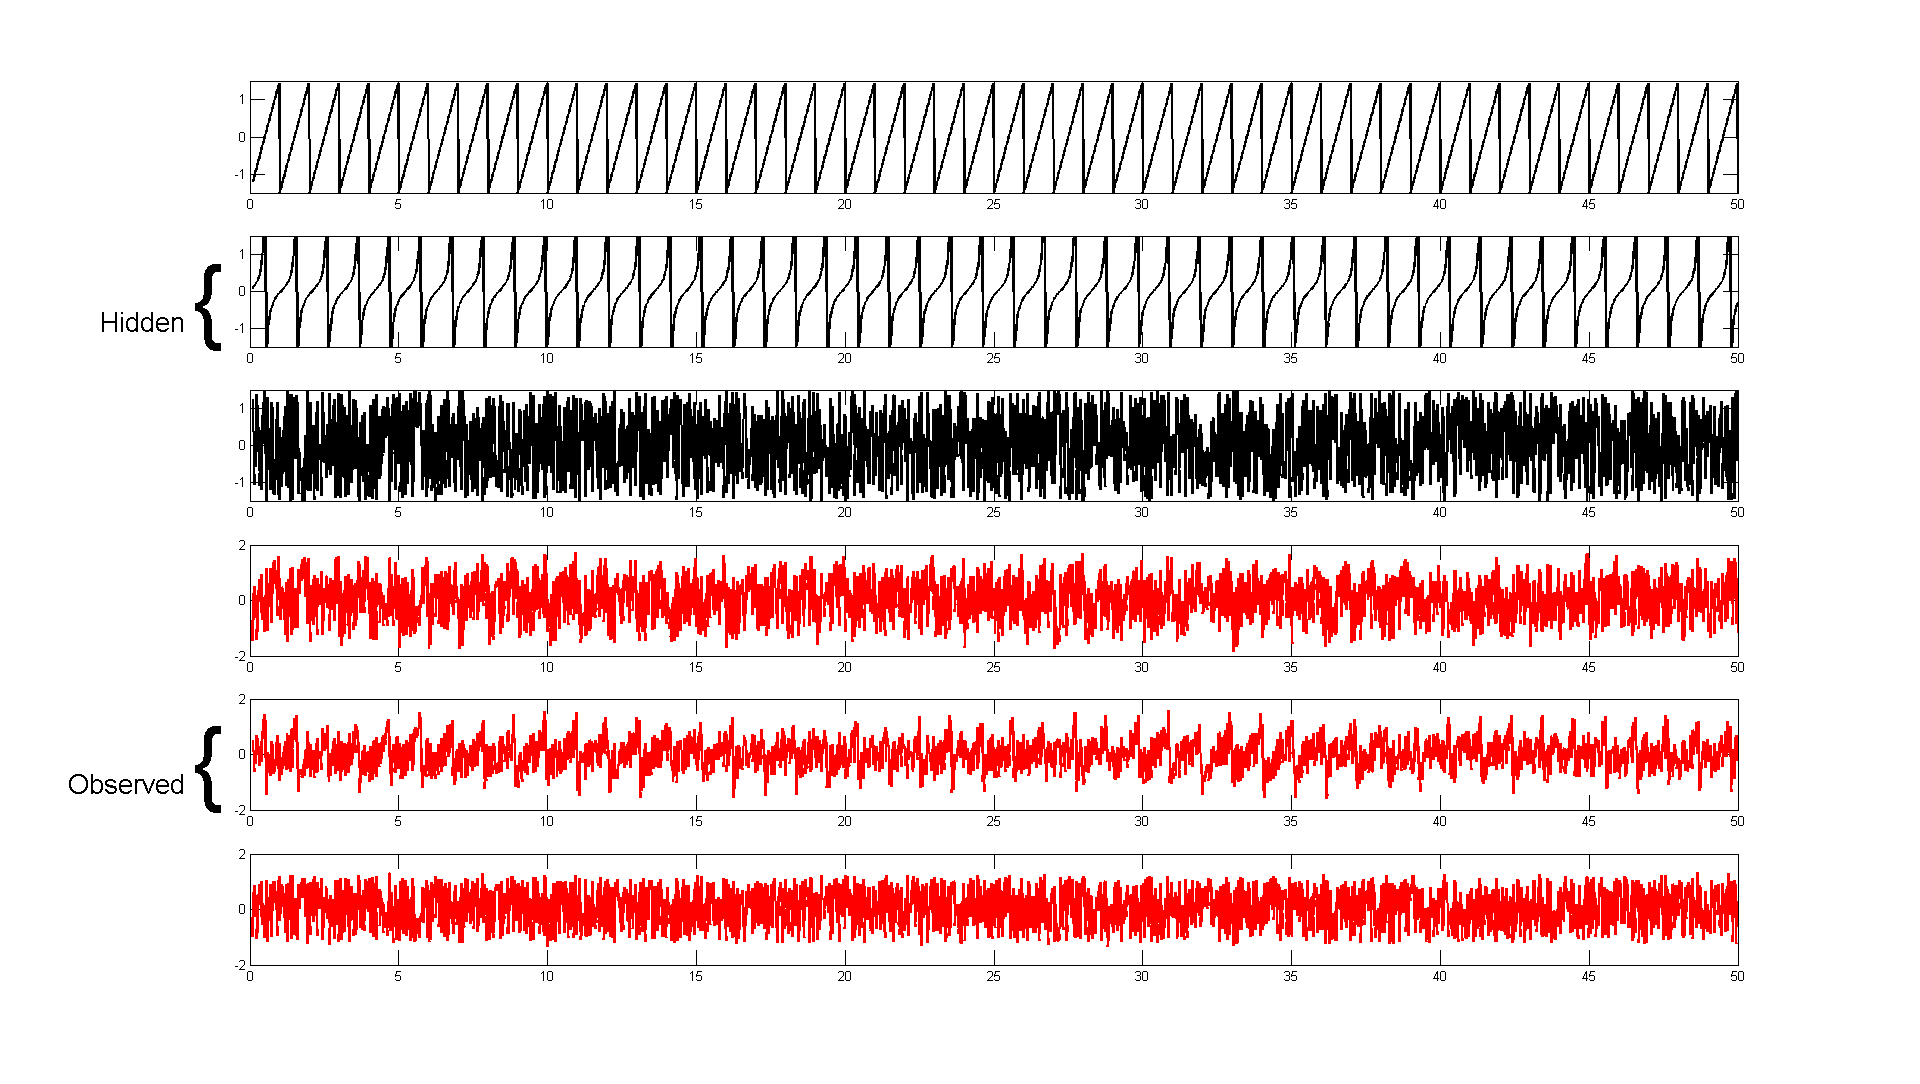
\includegraphics[width = 0.49\linewidth]{demo_source}
	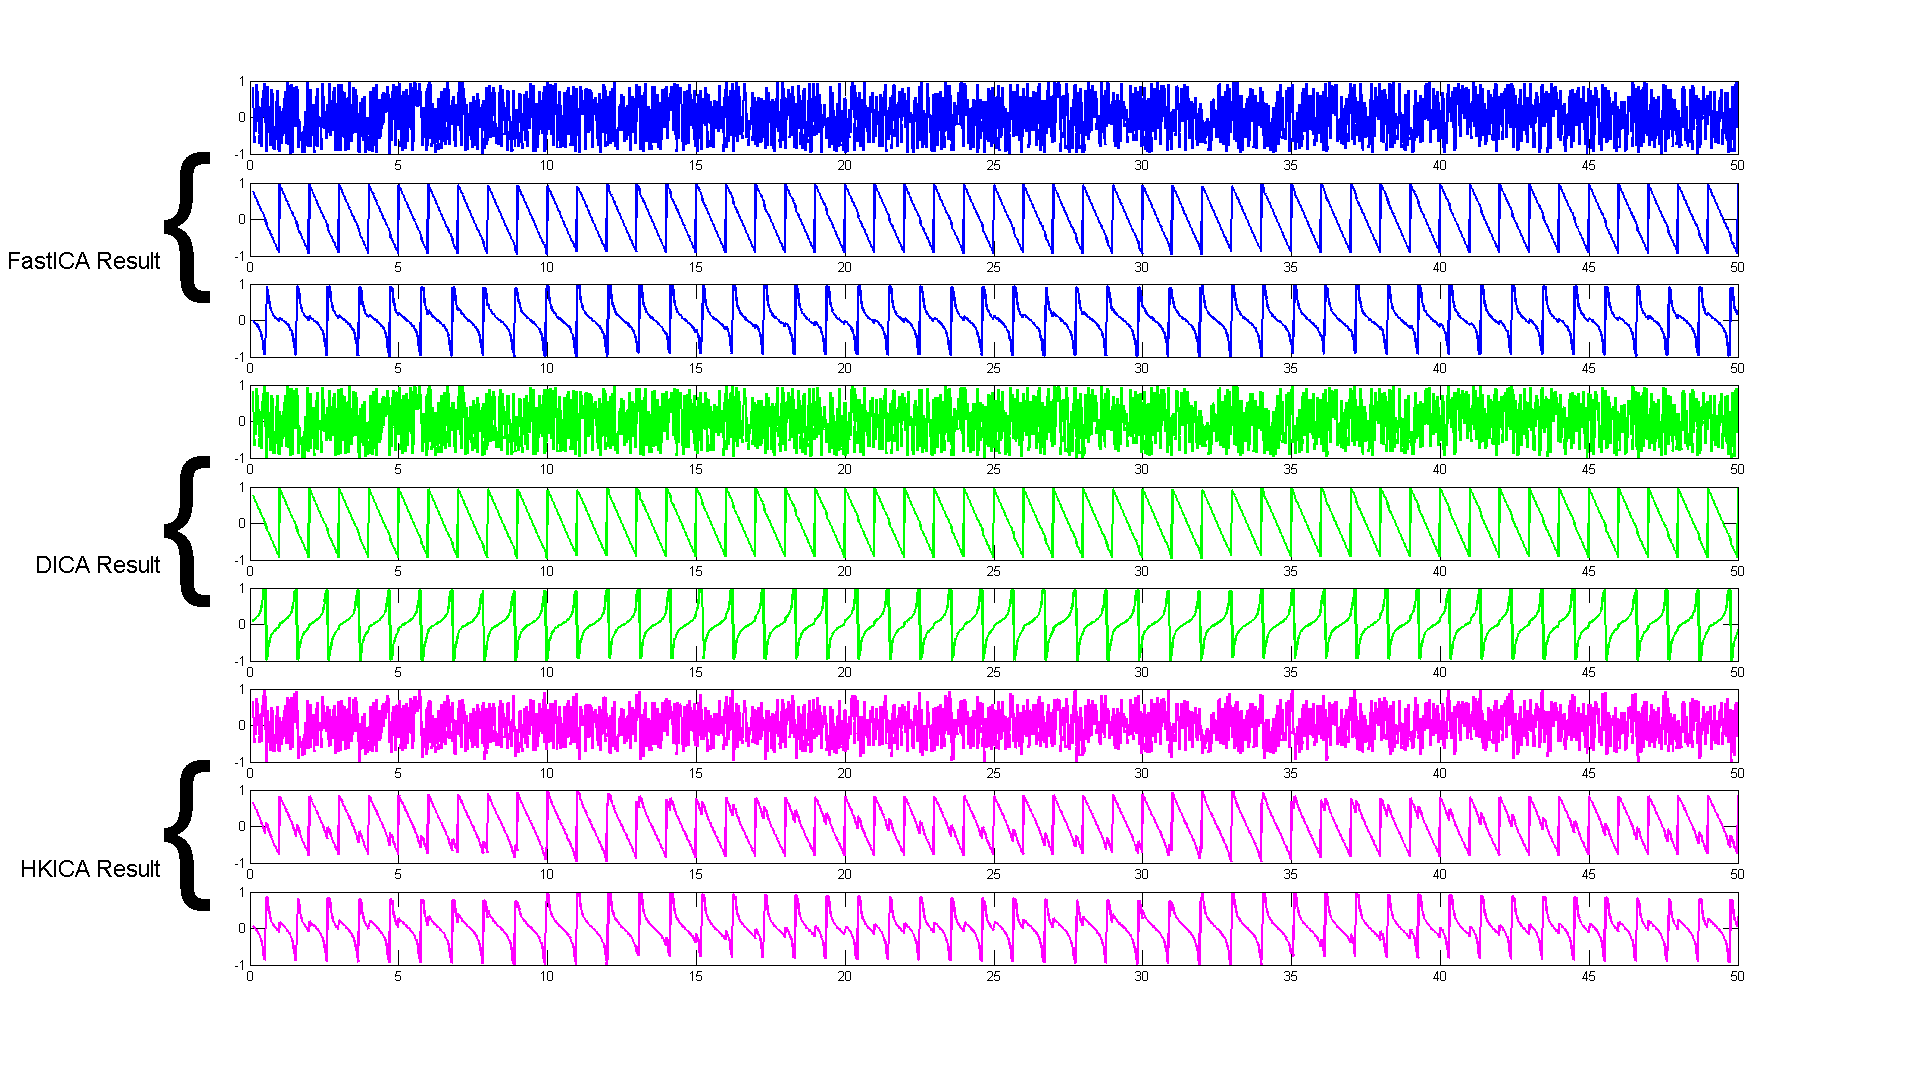
\includegraphics[width = 0.49\linewidth]{demo_res}
\caption{Example of ICA: On the left-hand side, the bottom three plots depict the $d=3$ components of the observed signal $x$. 
This observed data $x$ is generated by mixing the sources shown by the top three graphs on the left-hand side.
The $x$ axis represents time: The numbers shown are scaled by a factor of $50$; thus $T=2500$.
Reconstruction results by three algorithms (FastICA, HKICA, and DICA, see Section \ref{subsec:relatedWorks} and \ref{sec:DICA} for details)}
% after sampling $As(t)$ at 2500 uniformly spaced points in the interval $[0,50]$.}
\label{fig:demo}
\end{figure}
As can be seen, 
up to scaling and the ordering of the reconstructed components, the reconstruction is quite successful no matter the algorithms.
Note that the all components of the source data are periodic functions of time. 
This is quite obvious for the first two components, while the third, being generated using a pseudo-random number generator has a long period and thus ``looks random''.
Also, as the reader may recall, any two constant numbers $a,b \in \real$ are independent of each other when viewed as degenerate random variables. Thus, $s_1(t)$, $s_2(t)$, and $s_3(t)$ are independent. 
Does the success of the algorithms on this example implies that they will also work for other mixtures of deterministic sources? Of course not. 
For example, if one source is a linear function of other sources, then no algorithm will be able to recover the sources from their mixture.
 Another question is whether the temporal dependency of the sources may hamper the performance. 
If $s(1) = s(2) = \dots = s(T)$ then the algorithms effectively need to work with a single vector observation and no algorithm will be able to perform a successful reconstruction. 

In this paper, we attempted to provide some answers to the question: to what extents can ICA algorithms separate the mixture of some sources? 
In particular, can we redefine the problem of ICA in a meaningful way so tat we can explain the success of the particular ICA algorithms on the above example?
The essence of our approach is to define an empirical measure of the ``niceness'' of data and then postulating the requirement that good algorithms are those that get better results on `nice' data.
The niceness measure should behave in a controlled fashion in the classical ICA setting, so that the usual statistical results can be recovered from our results. 
We also propose a \emph{provably polynomial-time} algorithm for the noisy ICA model and analyze its performance based on the "niceness" of the observed data. 
The key feature of our approach is that no probabilistic assumptions are made on the data (the algorithm may randomize though), and thus this work can be thought as the natural extension of online learning
where learning algorithms are analyzed without making any probabilistic assumptions \citep{CBLu06:book}.


The rest of this paper is organized as follows: 
We review some previous works in the literature and compare them to our algorithm in Section \ref{subsec:relatedWorks}.
The ICA problem is introduced in detail in Section~\ref{sec:Preliminaries} and  our main results are highlighted in Section~\ref{sec:main}.
The polynomial-time algorithms underlying these results are developed through the next two sections: Section~\ref{sec:AnalysisHK} is devoted to the analysis of the HKICA algorithm, also showing its disadvantages, while our new algorithms are presented in Section~\ref{sec:DICA}.
Experimental results are reported in Section \ref{sec:ExpRes}.

\subsection{Related Works}
\label{subsec:relatedWorks}
We explain the difference between our ICA algorithm and the previous methods in this section. 
However, as mentioned above, the key feature of this paper is rather the removal of the probabilistic assumptions on the observed data.
 
A popular approach to the ICA problem is to find a linear transformation $W$ for $X$ by optimizing a \emph{contrast function} 
that measures dependence or non-gaussianity of the resulting coordinates of $WX$.
The optimal $W$ then can serve as an estimate of $A^{-1}$, thereby recovering the mixing matrix $A$.
One of the most popular ICA algorithms, FastICA \citep{hyvarinen1999fast},
follows this approach for a specific contrast function.  
FastICA has been analyzed theoretically from many aspects \citep{tichavsky2006performance,oja2006fastica,ollila2010deflation,dermoune2013fastica,wei2014convergence}.
In particular, recently \citet{miettinen2014fourth} showed  that in the noise-free case (i.e., when $X = AS$), the error of FastICA (when using a particular forth-moments-based contrast function) vanishes at a rate of $1/\sqrt{T}$ where $T$ is the sample size.
In addition, several other methods have been shown to achieve similar error rates in the noise-free setting \citep[e.g.,][]{eriksson2003characteristic,samarov2004nonparametric,chen2005consistent,chen2006efficient}.
However, to our knowledge, no similar finite sample results are available in the noisy case.

On the other hand, several promising algorithms are available in the noisy case that make significant advances towards provably efficient and effective ICA algorithms, albeit fall short of providing a complete solution. 
Using a quasi-whitening procedure, \citet{arora2012provable} reduces the problem to finding all the local optima of a specific function defined using the forth order cumulant, 
and propose a polynomial-time algorithm to find them with appealing theoretical guarantees. However, the results depend on an unspecified parameter ($\beta$ in the original paper) whose proper tuning is essential; note that even an exhaustive search over $\beta$ is problematic, since its valid range is not well understood.

The exploitation of the special algebraic structure of the forth moments induced by the independence leads to several other works related to ICA \citep{hsu2013learning,anandkumar2012tensordecomposition,anandkumar2012method}. 
A similar idea is also discussed earlier as a intuitive argument to construct a contrast function \citep{cardoso1999high}. 
The first rigorous proofs for this idea are developed using matrix perturbation tools in a general tensor perspective \citep{anandkumar2012tensordecomposition,anandkumar2012method,goyal2014fourier}. 
A common problem faced by these methods is a minimal gap of the eigenvalues, which may result in an exponential dependence on the number of source signals $d$.
More precisely, these methods all require an eigen-decomposition of some flattened tensor where the minimal gap between the eigenvalues plays an essential role. 
Although the exact size of this gap is not yet understood, a naive analysis introduces an exponential dependence on the dimension $d$. 
Such dependence is also observed in the literature \citep{cardoso1999high,goyal2014fourier}.
One way to circumvent such dependence is to directly decompose a high-order tensor using the power method, which requires no flattening procedure \citep{anandkumar2014guaranteed}. 
However, when applied to the ICA problem, this introduces a bias term and so the error does not approach 0 as the sample size approaches infinity.
Another issue is the well-known fact that the power method is unstable in practice for high-order tensors. 
\citet{goyal2014fourier} proposed another method by exploring the characteristic function rather than the forth moments.
However, their algorithm requires picking a parameter ($\sigma$ in the original paper) that is smaller than some unknown quantity, making their algorithm impossible to tune.
Recently, \citet{vempala2014max} proposed an ICA algorithm based on an elegant, recursive version of the method of \citet{goyal2014fourier} that avoids dealing with the aforementioned minimal gap; however, they still need an oracle to set the unspecified parameter of \citet{goyal2014fourier}.

Our ICA algorithm is a refined version of the ICA method proposed by \cite{hsu2013learning} (HKICA). 
However, we propose two simpler ways, one inspired by \citet{frieze1996learning}, \citet{arora2012provable}, and another based on \citet{vempala2014max}, to deal with the spacing problem of the eigenvalues under similar conditions to those of \citet{goyal2014fourier}.
Unlike the method proposed by \citet{goyal2014fourier}, our first method can force the eigenvalues to be well-separated with a gap that is independent of the mixing matrix $A$, while our second method, based on the recursive decomposition idea of \citet{vempala2014max}, avoids dealing with the minimum gap (on the price of introducing other complications).
We prove that our methods achieve an $O(1/\sqrt{T})$ error in estimating $A$ in the classical setting, with high probability, such that both the convergence rate and the computational complexity scale \emph{polynomially} with the natural parameters of the problem. 
Our method needs no parameter tuning, which makes it even more appealing. 


%Another contribution of the present paper is that our analysis is conducted in a deterministic manner. 
%In practice, ICA is also known to work well for unmixing the mixture of various deterministic signals. 
%One of the classical demonstrations of ICA is showing that two periodic signals can be well recovered from their mixtures \citep{HyvOja00}.
%Such an example is shown in Figure~\ref{fig:demo}. It can be seen that our algorithm, DICA, in this particular example, can solve the problem better than
%other algorithms, FastICA \citep{hyvarinen1999fast} and HKICA \citep{hsu2013learning}.


%\begin{figure}[pt]
%\captionsetup{singlelinecheck=off}
%\centering %
%	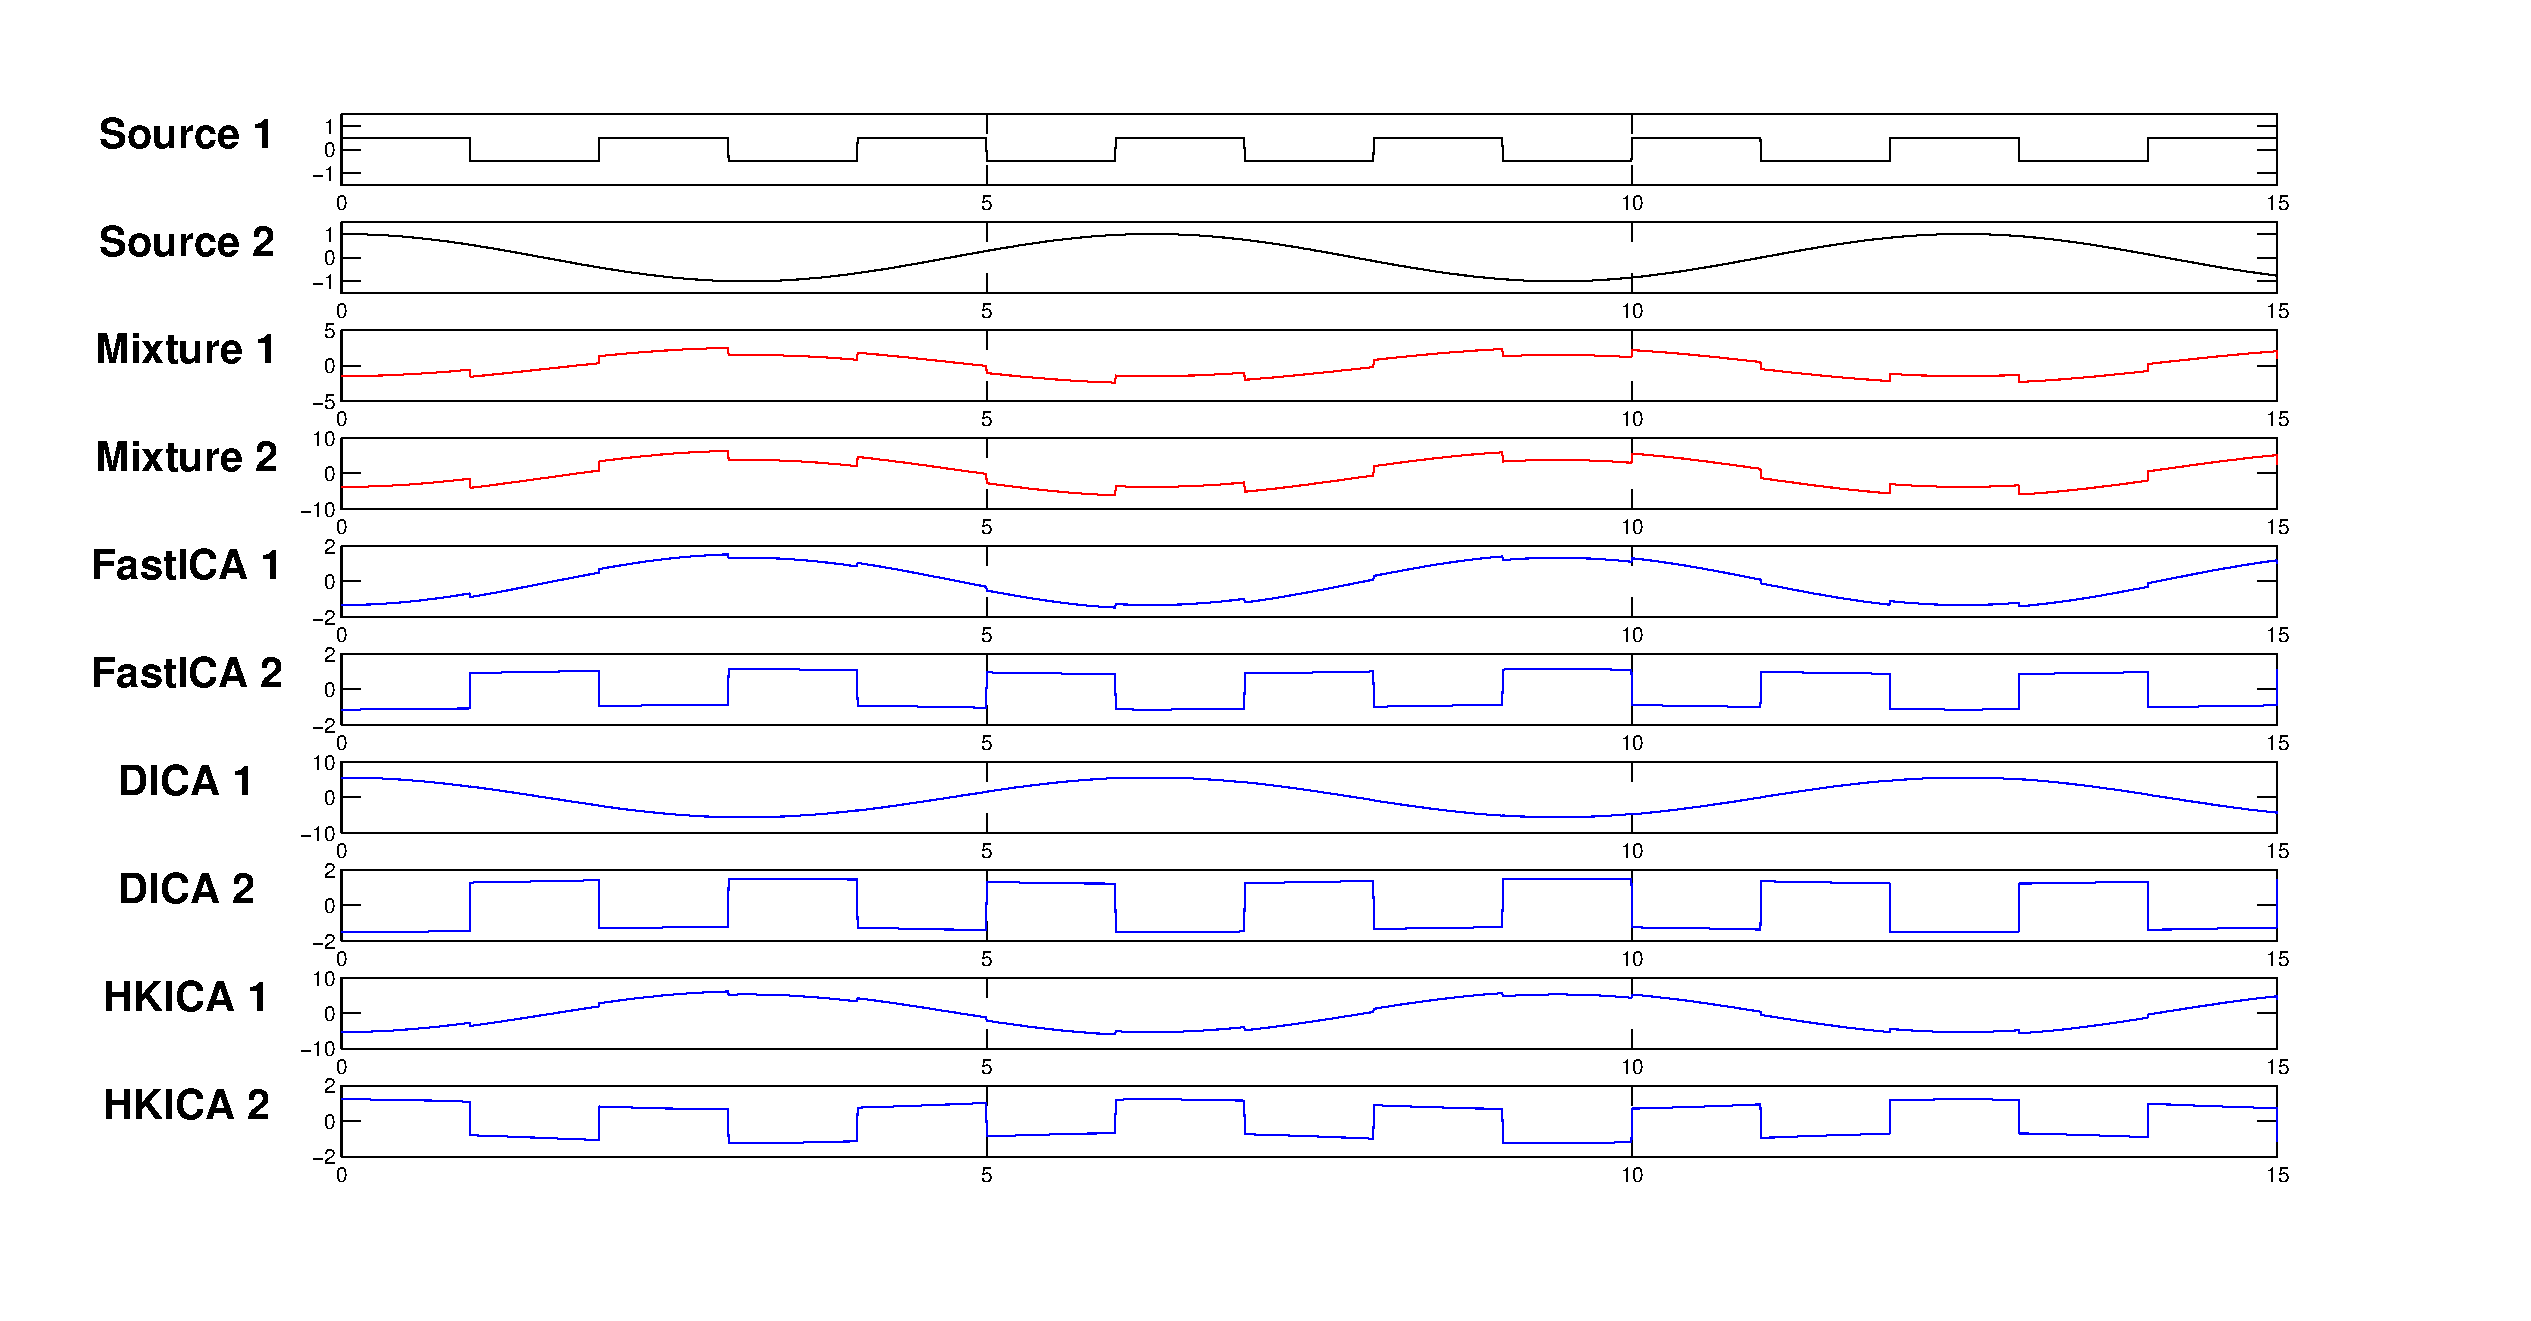
\includegraphics[width = 1.05\textwidth]{demo}
%\caption{Example of ICA for deterministic sources: The first two rows show the source signals
%$s_1(t)=0.5 - \lfloor t-2\lfloor t/2 \rfloor \rfloor$, 
%$s_2=\cos(t)$, the next two rows present the observations with mixing matrix 
%$A=\left(
%\protect\begin{array}{cc}
%1&-2\\
%2.6 & -5.1
%\protect\end{array}
%\right)$. 
%The reconstructed (and rescaled) signals are shown for FastICA, HKICA, and DICA after sampling $As(t)$ %at 3000 uniformly spaced points in the interval $\left[0,15\right]$.}
%\label{fig:demo}
%\end{figure}
%Such phenomenon suggests that the usual probabilistic notion is unsatisfactory if one wishes to have deeper understanding of ICA.   
%Our deterministic analysis helps investigate this curious phenomenon without losing any generality to the traditional stochastic setting. Formally, instead of observing $T$ \iid samples from \eqref{eq:stoch-ICA}, the source signals are defined by the function $s:\natural \ra \real^d$ be a $d$-dimensional deterministic ``signal'', and
%the observations are $x(t)=A s(t) +\epsilon_t$, where $(\epsilon_t)_{t=1}^\infty$ is an \iid sequence of $d$-dimensional $\mathcal{N}(0,\Sigma)$ random variables.

\subsection{Notation}
All vectors, matrices and tensors are real or complex valued, unless otherwise stated; below $K$ denotes either the set of real or complex numbers. We denote the set of real and natural numbers by $\real$ and $\natural$, respectively.
A vector $v \in K^d$ for a field $K$ is assumed to be a column vector.
Let $\|v\|_2$ denote its $L_2$-norm, and for any matrix $Z$ let $\|Z\|_2=\max_{v:\|v\|_2=1}{\|Z v\|_2}$ denote the corresponding induced norm. Denote the maximal and minimal singular value of $Z$ by $\sigma_{\max}(Z)$ and  $\sigma_{\min}(Z)$, respectively. Also, let $Z_i$ and $Z_{i:}$ denote the $i$th column and, resp., row of $Z$, and let $Z_{(2,\min)} = \min_{i} \|Z_i\|_2$, $Z_{(2,\max)} = \max_{i} \|Z_i\|_2$ and $Z_{\max} = \max_{i,j} |Z_{i,j}|$. 
Clearly, $\sigma_{\max}(Z) =\|Z\|_2 \ge Z_{(2,\max)} \ge Z_{\max}$, and $\sigma_{\min}(Z) \le Z_{(2,\min)}$. For a tensor (including vectors and matrices) $T$, its Frobenious norm (or $L_2$ norm) $\|T\|_F$  is defined as the square root of the sum of the square of all the entries.  
For a vector $v=(v_1,\ldots,v_d) \in K^d$, $\vert v \vert$ is defined coordinatewise, that is $\vert v \vert=(\vert v_1 \vert,\ldots,\vert v_d\vert)$. 
The transpose of a vector/matrix $Z$ is denoted by $Z^\top$, while the inverse of the transpose is denoted by $Z^{-\top}$.  
The outer product of two vectors $v, u \in K^d$ is denoted by $u\otimes v=u v^\top$. 
$v^{\otimes k}$ denotes the $k$-fold outer product of $v$ with itself, that is, $v\otimes v\otimes v \ldots \otimes v$, which is a k-dimensional tensor.
Given a $4$-dimensional tensor $T$, we denote the matrix $Z$ by $T(\eta,\eta,\cdot , \cdot)$ that is generated by marginalizing the first two coordinates of $T$ on the direction $\eta$, that is,
$Z_{i,j} = \sum_{k_1,k_2 = 1}^{d} \eta_{k_1} \eta_{k_2} T_{k_1,k_2,i,j}$. (Similar definitions for marginalizing different coordinates of the tensor.)
For a real vector $v$ and some real number $C$, $v \le C$ means that all the entries of $v$ are at most $C$. 
The bold symbol $\boldsymbol{1}$ denotes a vector with all entries being $1$ (the dimension of this vector will always be clear from the context).
Finally, $\poly{\cdot,\cdots,\cdot}$ denotes a polynomial function of its argument.

\section{Main Result}
\label{sec:main}
In this paper we consider the following non-stochastic version of the ICA problem.
Assume that we can observe a $d\times T$ segment of mixed signal $x(t) \in \R^d, t \in [T]:=\{1,2,\ldots,T\}$.
We consider the problem of reconstructing the $d\times d$ non-singular mixing matrix $A$ having observed $x$ provided that $(A,s,\eps)$ are ``nice''as defined later, and that 
\begin{equation}
\label{eq:ICA}
x(t) = As(t)+\epsilon(t), \qquad 1\le t\le T\,.
\end{equation}
Intuitively, $s$ is the source whose components are ``independent'' while $\epsilon$ is ``noise''.
We measure how well a matrix $\hat{A}$ returned by an algorithm working on data $x$ 
recovers $A$ by the reconstruction error defined as
\[
d(\hat{A}, A) = \inf_{
		\substack{\pi \in \mathrm{Perm}([d]) \\ c\in \real^d}} 
		\max_{k} || c_k \hat{A}_{:\pi(k)} - A_{:k} ||_2\,,
\]
where $A_{:i}$ stands for the $i$th column of $A$ and
$\mathrm{Perm}([d])$ is the set of all the permutations on the set $[d]$.
This measure compensates for the inherent indeterminacy in reconstructing the scale and ordering of sources.
Furthermore, we will use the notation $\sigma_{\min}=\sigma_{\min}(A)$ and
$\sigma_{\max}=\sigma_{\max}(A)$.

Let us now develop the ``niceness'' measure of the $(x,A,s,\eps)$. 
Starting from the classical setting, we will define this tuple nicer if the respective \emph{empirical} 
distributions approximately satisfy the usual assumptions: 
\begin{enumerate}[(a)]
\item the source ($s$) components are independent;
\item the noise and source are independent.
\item the source ($s$) have high absolute $4^{\rm th}$-order cumulants (kurtosis);
\item the noise ($\eps$) has low absolute $4^{\rm th}$-order cross cumulants;
\item the source ($s$) have zero mean;
\item the noise ($\eps$) has  zero mean;
\end{enumerate}

To measure the degree of independence of the components of the source $s$, we define
a family of ``distances'' between distributions (strictly speaking, these are only pseudo-distances).
In particular, given two distributions $\nu_1$ and $\nu_2$ over $\real^d$ and an integer $k\ge 1$, we
let $D_k(\nu_1,\nu_2) = \sup_{f\in\mathcal{F}} |\int f(s)\nu_1(ds) - \int f(s)\nu_2(ds)|$, 
where $\mathcal{F}=\{f:\real^d \to \real : f(s)=\prod_{j=1}^k s_{i_j}, 1 \le i_1,\ldots,i_k \le d\}$ 
is the set of all monomials up to degree $k$.
When $\mu$ is a product measure, $D_k(\mu,\nu)$ measures how close the components of $X\sim \nu$ are to being independent.
When $\nu$ is a measure of $p+q$ variables (i.e., $X\in \real^{p+q}$) 
we also need a measure that quantifies the degree of independence of the vectors $(X_1,\dots,X_p)$ and $(X_{p+1},\dots,X_{p+q})$. We will denote this measure by $D_k^{(p,q)}(\nu)$ and is defined as $D_k^{(p,q)} (\nu)= \inf_{\mu_1,\mu_2} D_k(\mu_1\otimes \mu_2,\nu)$, where $\mu_1$ ranges over all measures on $\real^p$ and $\mu_2$ ranges over all measures on $\real^q$. 
As can be seen later, $D_k^{(p,q)}(\nu)$ will be used to measure the independence between the source ($s$)) and the noise ($\eps$).

For any $t,k \ge 1$ and signal $u:[t] \to \R^k$, we introduce the empirical distribution $\nu_t^{(u)}$ defined by
$\nu_t^{(u)}(B)=\tfrac{1}{t}|\{\tau \in [t]: u(t) \in B\}|$ for all Borel sets $B \subset \R^k$. 
For a distribution $\mu$ over the reals we let $\kappa(\mu)$ be the (absolute) $4^{\rm th}$-order cumulant of $\mu$: 
$\kappa(\mu) = |\int x^4 \mu(dx) - 3 (\int x^2 \mu(dx))^2|$, which, for brevity, we also call ``kurtosis'' (by slightly abusing terminology).
For a product distribution $\mu= \mu_1\otimes \ldots \otimes \mu_d$ over $\real^d$, we let $\kappa_{\min}(\mu)
=\min_{1\le i \le d} \kappa(\mu_i)$ to denote the minimum kurtosis of the components of $\mu$.
When $\mu$ is a distribution over $\real^d$, we define the $d$-dimensional absolute 
$4^{\rm th}$-order cumulant of $\mu$ by 
%\todoc{I wonder if this should be $M_{i,j,k,l} - (M_{i,j}M_{k,l} + M_{i,k}M_{j,l} + M_{i,l}M_{j,k})$, as show e.g. in \citep{Lee98:ICAbook} page 23.}
$\cQ(\mu) = \max_{\|\eta\|_2 \le 1}\| \left(\E_{Y\sim \nu_t^{(\epsilon)}} [Y^{\otimes4}] - (\E_{Y\sim \nu_t^{(\epsilon)}} [Y^{\otimes2}])^{\otimes 2}\right)(\eta,\eta,\cdot,\cdot)  - 2 (\E_{Y\sim \nu_t^{(\epsilon)}} [Y^{\otimes2}])^{\otimes 2}(\eta,\cdot,\eta,\cdot)\|_F $.

We will also use $N(\nu) = \|\int x \nu(dx)\|_F$ to denote the mean of the distribution $\nu$. Finally, we let 
\[
L = \max \left( \| \textstyle\int  [y^{\otimes 2}] \nu^{(\epsilon)}(dy) \|_F,\, 
			  \| \int  [y^{\otimes 3}] \nu^{(\epsilon)}(dy) \|_F \right),
\]
which captures the magnitude of second and third moments of the noise.
We let $\Pi_0$ to be the set of zero mean product distributions over $\real^d$. 

Now we are ready to state our main result. The algorithm that achieves this bound will be described later in the paper.

\begin{theorem}
\label{thm:finalRes} 
There exists a randomized algorithm such that 
for any $A\in \real^{d\times d}$, and $x, s, \epsilon: [T] \rightarrow \real^d$ satisfying Equation \eqref{eq:ICA},
the algorithm returns $\hat{A}$
%Consider the ICA problem \eqref{eq:ICA}. There exists an algorithm that estimates the mixing matrix $A$ from $T$ samples of $x$ 
such that with probability at least $1-\delta$,
\[
d(\hat{A}, A) \le
\inf_{\mu\in \Pi_0} \mathcal{C}(\mu) \min\left(D_4(\nu^{(s)},\mu)+ \cQ(\nu^{(\eps)}) + D_4^{(d,d)}(\nu^{(As,\eps)})
+N(\nu^{(\eps)}) + N( \nu^{(s)}), \Theta(\mu) \right),
\]
where $\mathcal{C}(\mu)$ and $\Theta(\mu)$ are problem dependent constants, polynomial in $(\sigma_{\max}(A), 1/\sigma_{\min}(A), 1/\kappa_{\min}(\mu),1/\delta, d, L)$.
Further, the computational complexity of the algorithm is $O(d^3 T)$ when used on any data $x$ of dimensions $T\times d$.
\end{theorem}
\begin{remark}
Our algorithms are randomized algorithms. The high probability $1-\delta$ in the first part of Theorem \ref{thm:finalRes} comes from the random sampling of the algorithm. The observations are deterministic and thus has no randomness. 
\end{remark}

\begin{remark}
The dependence on $\delta$ in our result is $\poly{\frac{1}{\delta}}$, which is weaker than the usual $\log(\frac{1}{\delta})$.
\end{remark}

\subsection{Applicability of Theorem \ref{thm:finalRes}}
Theorem \ref{thm:finalRes} can be applied to a variety of different ICA settings.
\begin{proposition}
\label{prop:stochasticAss}
In the classical stochastic setting of ICA, i.e. when $(s(t))_{t\in[T]}$ is an \iid sequence, independent of the \iid Gaussian noise sequence $(\epsilon(t))_{t\in[T]}$, with probability at least $1-\delta$, $L = \poly{A_{\rm max}, \|\Sigma\|_2,C,d,\frac{1}{\delta}}$.
Moreover, if $\mu$ is the product measure of the sources, then $D_4(\nu^{(s)},\mu)$, $\cQ(\nu^{(\eps)})$, $D_4^{(d,d)}(\nu^{(As,\eps)})$, $N(\nu^{(\eps)})$, $N(\nu^{(s)})$ are all in a rate of $\frac{1}{\sqrt{T}}$.
\end{proposition}
Note that the above result implies that in the standard stochastic setting
with independent sources and Gaussian noise, independently generated from the sources, 
with probability at least $1-\delta$,
\[
d(\hat{A}, A) \le \mathcal{C} \min\left(\tfrac{1}{\sqrt{T}}, \Theta \right),
\]
for some problem dependent constants $\mathcal{C}$ and $\Theta$.

Our setting can also cover some other examples excluded by the traditional setting, such as the example of Figure~\ref{fig:demo} in Section~\ref{sec:Intro}.
\begin{example} \em
\label{ex:periodic}
Assume that the unknown sources $s_i$ ($1\le i\le d$) are deterministic and periodic. Our observation $x=As+\eps$ is a linear mixture of $s$ contaminated by i.i.d.\ Gaussian noise for each time step, where $A$ is a non-singular matrix and $\eps\sim {\cN}(0,\Sigma)$ is Gaussian.   
Even though $\eps$ is i.i.d.\ for every time step, the observations cannot satisfy the traditional i.i.d.\ assumption, since the source $s$ is deterministic. 
However, it can be proved that if the ratio of the periods of each pair of $(s_i, s_j)$ is irrational, then the reconstruction error would approach 0 for $T$ large enough.   
\end{example}
\begin{remark}
To have a concrete (noise-free) example, let $s_1(t)=0.5 - \lfloor t-2\lfloor t/2 \rfloor \rfloor$, $s_2=\cos(t)$. 
It is easy to see that the limit distribution of source 1 is a Bernoulli distribution $\mu_1$ with $\mu_1(\{0.5\}) = 1/2$ and $\mu_1(\{-0.5\}) = 1/2$, and the limit distribution of source 2 is a distribution $\mu_2$ with density function $p(x) = \frac{1}{\pi \sqrt{1-x^2}}$ for $-1\le x \le 1$.
Pick $\mu = \mu_1 \otimes \mu_2$.
Let $T = 2*u + b$ as the division with remainder, where $u$ is integer and $0\le b<2$. 
Moreover, assume $b\le 1$ (similar analysis will go through for the case of $b>1$).  
The induced distribution $\nu_T^{s_1}$ of source 1 is $\nu_T^{s_1}(\{0.5\}) = \frac{u+b}{T}$ and $\nu_T^{s_1}(\{-0.5\}) = \frac{u}{T}$. 
Thus the total variation distance of $\mu_1$ and $\nu_T^{s_1}$ is at most $1/(2T)$. 
Similarly, it can be verified that the total variation distance of $\nu_T^{s_2}$ and $\mu_2$  and that of $\nu_T$ and $\mu$ also decay as $1/T$. 
Thus, $D_4$ is $O(1/T)$, since the monomials $f(s)$ in the definition
of $D_4$ are bounded from above by $1$, and $N(\nu^{(s)})$ is also $O(1/T)$.
Therefore we achieve an error rate of $\frac{1}{T}$.
\end{remark}
Our setting also extends the traditional one to a practically important case, Markov sources.  
\begin{example} \em
\label{ex:markov}
Assume that $s_i$ is a stationary and ergodic Markov source, and the sources are independent of each other for $1\le i\le d$. Our observations are similar to the setting in Example \ref{ex:periodic}. 
Because of the Markov property, the observations do not satisfy the i.i.d. assumptions.
\end{example}

In the next sections, we will present two algorithms that satisfy Theorem \ref{thm:finalRes}.

\section{A ``Deterministic'' ICA Algorithm}
Our algorithm builds on the works of \citet{frieze1996learning,hsu2013learning,arora2012provable}. In this section we will first introduce the ICA algorithm of  \citet{hsu2013learning} and analyze its performance.
The result suggests a dependence on a spacing problem that is dependent on the mixing matrix $A$ and difficult to analyze.
Such problem motivates us to refine the algorithm, which leads to our algorithm, deterministic ICA (DICA). 

\subsection{Estimating Moments: the HKICA Algorithm}
\label{sec:HKICA}
The ICA algorithm of \citet{hsu2013learning} is based on the well-known excess-kurtosis-like quantity
defined as follows:

For any $p\ge 1$, $\eta\in \real^d$, and distribution $\nu$ over $\R^d$,
let 
\begin{equation}
\label{eq:momnent}
m_p^{(\nu)}(\eta) = \E_{X\sim \nu}[ (\eta^\top X)^p ]
\end{equation}
and let
\begin{equation}
\label{eq:funcf}
f_{\nu}(\eta) = \frac1{12} \left( m_4^{(\nu)}(\eta) - 3 m_2^{(\nu)}(\eta)^2 \right)\,.
\end{equation}
\citet{hsu2013learning} showed that $\nabla^2f_{\nu_T^{(x)}}(\eta)$, the second derivative of the function $f_{\nu_T^{(x)}}$, is extremely useful for the ICA problem:
They showed that if $\mu^{(X)}$ is the distribution of the observations $X$ in the stochastic setting where $S$ comes from the product distribution $\mu$, then
$f_{\mu^{(X)}}(\eta)=f_{A\mu}(\eta)$ for all $\eta$ (where $A\mu$ denotes the distribution of $AS$) and, consequently, the eigenvectors\footnote{Throughout the paper eigenvectors always mean right eigenvectors, unless specified otherwise.} of the matrix $M=\nabla^2f_{\mu^{(X)}}(\phi)(\nabla^2f_{\mu^{(X)}}(\psi))^{-1}$ are the rescaled columns of $A$ if $\frac{\phi^\top A_i}{\psi^\top A_i}$ are distinct for all $i$. 
Thus, to obtain an algorithm, one needs to estimate $\nabla^2 f_{\mu^{(X)}}$ in such a way that the noise $\epsilon$ could still be neglected.

An estimate $\nabla^2 \hat{f}$ of $\nabla^2f_{\mu^{(X)}}$ is not hard, since for any $\nu$,
$\nabla^2f_{\nu}(\eta)$  can be computed as
\begin{equation}
\label{eq:G}
\nabla^2 f_{\nu}(\eta) = G_{\nu}(\eta):= G_1^{(\nu)}(\eta) - G_2^{(\nu)}(\eta) -2G_3^{(\nu)}(\eta),
\end{equation}
where 
\begin{align*}
& G_1^{(\nu)}(\eta) =  \E_{X\sim \nu} [\big(\eta^{\top}X\big)^2XX^{\top}]; \\
& G_2^{(\nu)}(\eta) = \E_{X\sim \nu} [\big(\eta^{\top}X\big)^2] \E_{X\sim \nu} [XX^{\top}]; \\
%\frac{1}{T^2}\sum_{t=1}^{T} \big(\eta^{\top}x(t)\big)^2 \sum_{t=1}^{T}x(t)x(t)^{\top}; \\
& G_3^{(\nu)}(\eta) = \E_{X\sim \nu} [\big(\eta^{\top}X\big)X] \E_{X\sim \nu} [\big(\eta^{\top}X\big)X^{\top}],
%\frac{1}{T^2}\Big(\sum_{t=1}^{T} \big(\eta^{\top}x(t)\big)x(t)\Big) \Big(\sum_{t=1}^{T} \big(\eta^{\top}x(t)\big)x(t)\Big)^{\top}.
\end{align*} 
and these quantities can be estimated using the observed samples. In what follows, we will use the estimate $\nabla^2 \hat{f}:=\nabla^2 f_{\nu_T^{(x)}}$ and, in general, we will add a ``hat'' to quantities which are derived from the empirical distribution $\nu_T^{(x)}$. 
%A un-hatted notion is estimated w.r.t. some product measure $\mu$. 
It is important to note that, under our assumptions, the noise $\epsilon$ has limited effect in the estimation procedure, as shown in the following proposition. 
Similar result is also discussed by \citet{arora2012provable} and \citet{belkin2013blind}.

\begin{proposition}
 \label{prop:denoise}
 Suppose Assumptions~\ref{ass:gauss} and~\ref{ass:independence} hold. Then,
for any vector $\eta$ satisfying $\|\eta\|_2\le L_{\eta}$,
\[
\| \nabla^2f_{\nu_T^{(x)}}(\eta) - \nabla^2f_{\nu_T^{(As)}}(\eta) \|_2 \le \text{Poly}(L_{\eta}, L, d, \sigma_{\max}, C)(g(T)+1)g(T). 
\] 
\end{proposition}

In particular, the difference in the estimation of the Hessian matrix caused by the noise is $\poly{L_{\eta}, L, d, \sigma_{\max}, C}\left(g(T)+1\right)g(T)$.
Denote this quantity by $P(L_{\eta})$. 
Note that this error caused by the noise decays at a rate of $\sqrt{T}$.
Putting everything together, we obtain the algorithm HKICA, named after \citet{hsu2013learning}, which is shown in Algorithm~\ref{alg:HKICA},
\begin{algorithm}[H]
\caption{The HKICA algorithm.}
\label{alg:HKICA}
\begin{algorithmic}[1]
\INPUT $x(t)$ for $1\le t \le T$. 
\OUTPUT An estimation of the mixing matrix $A$. 
\STATE Sample $\phi$ and $\psi$ independently from a standard Gaussian distribution of dimension $d$;
\STATE Evaluate $\nabla^2\hat{f}(\phi)$ and $\nabla^2\hat{f}(\psi)$, 
\STATE Compute $\hat{M} = (\nabla^2 \hat{f}(\phi))(\nabla^2\hat{f}(\psi))^{-1}$;
\STATE Compute all the eigenvectors of $\hat{M}$, $\{\mu_1,\ldots,\mu_d\}$;
\STATE Return $\hat{A} = (\mu_1,\ldots,\mu_d)$.
\end{algorithmic}
\end{algorithm}

\begin{remark}
\label{rmk:symmetrization} 
Although in theory, HKICA generates a valid, real output almost surely, in practice this may not happen always as, due to numerical errors, $\nabla^2\hat{f}(\psi)$ may become singular or the ratio $(\phi^\top A_i)/(\psi^\top A_i)$ may become the same for multiple indices $i$. A simple way to fix this problem is re-sampling $\phi$ and $\psi$ until a real eigen-decomposition exists.
\end{remark}


\subsection{Analysis of HKICA}
\label{sec:AnalysisHK}
\citet{hsu2013learning} claimed that HKICA is easy to analyze using matrix perturbation techniques. In this section we provide a rigorous analysis of the algorithm, which reveals some unexpected complications.
\begin{definition}
Let $\Epsi$ denote the following event: For some fixed $0\le \ell\le 1$, let $\ell_l = \frac{\sqrt{\pi}A_{(2,\min)}}{\sqrt{2}d} \ell$, and $ L_u \ge \sqrt{2d}$,
$\min_i |\psi^{\top}A_i| \ge \ell_l$ and $\|\psi\|_2 \le L_u$ hold simultaneously. 
\end{definition}
Let 
\begin{equation}
\label{def:kappa}
\gamma_A =  \min_{i,j: i\neq j} \left\vert \left(\frac{\phi^{\top}A_i}{\psi^{\top}A_i}\right)^2 - \left(\frac{\phi^{\top}A_j}{\psi^{\top}A_j}\right)^2 \right\vert. 
\end{equation}

The performance of the HKICA algorithm will essentially depend on this parameters, as shown in the following theorem.
\begin{theorem}
\label{thm:efficiency} 
Suppose Assumptions~\ref{ass:gauss} and~\ref{ass:independence} hold. 
Furthermore, assume that
\begin{align*}
T & \ge \poly{d, L_u, C, \sigma_{\max},\kappa_{\max}, L,\frac{1}{\ell}, \frac{1}{\kappa_{\min}}, \frac{1}{\sigma_{\min}}, \frac{1}{\gamma_A}},
\end{align*}
and that there exist a product measure $\mu$ such that 
\[
\xi \le \poly{\gamma_A, \frac{1}{d}, \frac{1}{L_u}, \frac{1}{\sigma_{\max}}, \frac{1}{\kappa_{\max}}, \kappa_{\min}, \sigma_{\min}, \ell}.
\] 
Then, on the event $\Epsi$, there exists a permutation $\pi$ and constants $\{c_1,\ldots,c_d\}$, such that for any $k$,
\begin{equation}
\label{eq:HKICA-bound}
  \max_{1\le k\le d}\| c_1\hat{A}_{\pi(k)} - A_k\|_2 \le
  % \frac{4}{\gamma_A} \frac{\sigma_{\max}^2(A)}{ \sigma_{\min}}Q,
  \frac{1}{\gamma_A} (\xi + P(L_u))Q
\end{equation}
where $\hat{A}$ is the output of the HKICA algorithm, and 
\[Q=\poly{d, L_u, \sigma_{\max}, \kappa_{\max}, \frac{1}{\kappa_{\min}}, \frac{1}{\sigma_{\min}}, \frac{1}{\ell}}.\]
\end{theorem}
\begin{remark}
(i) Note that the bound in \eqref{eq:HKICA-bound} goes to zero at an $O(1/\sqrt{T})$ rate whenever $D_4(\mu,\nu_T^{(s)})=O(1/\sqrt{T})$ and $g(T) = O(1/\sqrt{T})$, as, e.g., in the stochastic setting.
(ii) The parameter $1/\gamma_A$ is essential in the above theorem, in the sense that not only the reconstruction error bound is linear in $1/\gamma_A$, but the condition also requires a small $1/\gamma_A$ so that the above error bound is valid. 
Also, since $\gamma_A$ is the minimum spacing of the eigenvalues of $M=\nabla^2 f_{A\mu}(\phi) (\nabla^2 f_{A\mu}(\psi))^{-1}$, the eigenvalue perturbations imposed by the noise cannot be too large compared to $\gamma_A$ without potentially  ruining the eigenvectors of $M$; thus, the dependence on $\gamma_A$ seems necessary.
\end{remark}

Despite the important role that $\gamma_A$ plays in the efficiency of the HKICA algorithm, it is not clear how it depends on different properties of $A$.
To the best of our knowledge, even a polynomial (in the dimension $d$) lower bound of $\gamma_A$ is not yet available in the literature. 
Similar problems have been discussed by  \citet{husler1987minimal} and \citet{goyal2014fourier}, but there solutions are not applicable to our case.

\section{A Refined HKICA Algorithm}
\label{sec:DICA}

The problems with $\gamma_A$ motivate us to refine the HKICA algorithm.
The idea is inspired by \citet{arora2012provable} and \citet{frieze1996learning} using a quasi-whitening procedure:

One can show that $\nabla^2 f_\mu(\psi)=A K D_{\psi} A^\top$ where $D_{\psi} =\text{diag}\left((\psi^{\top}A_1)^2,\cdots, (\psi^{\top}A_d)^2\right)$,
and so $B= AK^{1/2}D_{\psi}^{1/2}R^{\top}$ for some orthonormal matrix $R$. Defining $T_i=\nabla^2 f_\mu(B^{-\top} \phi_i)$, one can calculate that
$T_i=A K^{1/2} D_\psi^{-1/2} \Lambda_i A^\top$ where $\Lambda_i =\text{diag}\left( (\phi_i^\top R_1)^2,\ldots,(\phi_i^\top R_d)^2 \right)$ and $R_i$ denote the $i$th column of $R$.
Then $M=T_1 T_2^{-1} = A\Lambda A^{-1}$ with $\Lambda=\Lambda_1 \Lambda_2^{-1}=\text{diag}\left( \left(\frac{\phi_1^\top R_1}{\phi_2^\top R_1}\right)^2,\ldots,\left(\frac{\phi_1^\top R_d}{\phi_2^\top R_d}\right)^2 \right)$. Thus, $A_i$ are again the eigenvectors of $M$, but now the eigenvalues of $M$ are defined in terms of the orthogonal matrix $R$ instead of $A$,
and so the resulting minimum spacing
\vspace{-4mm}
\begin{equation}
\label{def:gammaR}
\gamma_R =  \min_{i,j: i\neq j} \left\vert \left(\frac{\phi_1^{\top}R_i}{\phi_2^{\top}R_i}\right)^2 - \left(\frac{\phi_1^{\top}R_j}{\phi_2^{\top}R_j}\right)^2 \right\vert
\end{equation}
is much easier to handle.

The resulting algorithm, called Deterministic ICA (DICA), is shown in Algorithm \ref{alg:DICA}. 
\begin{algorithm}
\caption{Deterministic ICA (DICA)}
\label{alg:DICA}
\begin{algorithmic}[1]
\INPUT $x(t)$ for $1\le t \le T$. 
\OUTPUT An estimation of the mixing matrix $A$. 
\STATE Sample $\psi$ from a $d$-dimensional standard Gaussian distribution;
\STATE Evaluate $\nabla^2\hat{f}(\psi)$, \\
%\quad where $\hat{m_p}(\eta) = \frac{1}{T}\sum_{k=1}^{T} (\eta^{\top}g(k))^p$, and $\hat{f}(\eta) = \frac{1}{12}\big(\hat{m_4}(\eta) - 3\hat{m_2}(\eta)^2 \big)$;
\STATE Compute the SVD of $\nabla^2\hat{f}(\psi) = U \Sigma V^{\top}$, and let $\hat{B} =  U \Sigma^{1/2}$.
\STATE Sample $\phi_1$ and $\phi_2$ independently from the standard Gaussian distribution;
\STATE Compute $\hat{T}_1 =\nabla^2\hat{f}(\hat{B}^{-\top}\phi_1)$ and  $\hat{T}_2 =\nabla^2\hat{f}(\hat{B}^{-\top}\phi_2)$;

\STATE Compute all the eigenvectors of $\hat{M} = \hat{T}_1\left(\hat{T}_2\right)^{-1}$, $\{\mu_1,\ldots,\mu_d\}$;
\STATE Return $\hat{A} = \{\mu_1,\ldots,\mu_d\}$.
\end{algorithmic}
\end{algorithm}
\begin{remark}
Similarly to HKICA, in theory DICA fails with probability 0 (giving, e.g., complex outputs), but this may be experienced due to numerical errors.
The same resampling trick can be applied again, as in Remark \ref{rmk:symmetrization}. 
\end{remark}

The DICA algorithm can be showed to have provable performance guarantees under some good events defined as follows:
\begin{definition}
Let $\Ephi$ denote the following event:
For some fixed constants $0\le \ell\le 1$ and $L_u \ge \sqrt{2d}$, let $\ell_l = \frac{\sqrt{\pi}}{\sqrt{2}d}\ell$,
% = \sqrt{2}\left(x^{1/2}+\sqrt{d}\right)$ for $x>0$,
$\|\phi_1\|_2 \le L_u$, $\|\phi_2\|_2 \le L_u$, and $\min_i \{|\phi_2^{\top}R_i|\} \ge \ell_l$ hold simultaneously. 
\end{definition}  
Similarly to Theorem~\ref{thm:efficiency}, one can show that under some technical assumptions, which 
hold with probability 1 if $\xi$, $P(L_u)$, and $P\left(\frac{\sqrt{3}L_u}{\sqrt{2}\sigma_{\min}\kappa_{\min}^{1/2}C_1}\right)$  are small enough,
on the event $\Epsi \cap\Ephi$,  there exists a permutation $\pi$ and constants $\{c_1,\ldots,c_d\}$, such that for $1\le k\le d$,
\[
\| c_k\hat{A}_{\pi(k)} - A_k\|_2 \le \frac{4\sigma^2_{\max}}{\gamma_R\sigma_{\min}} (\xi + P(L_u))Q,
\]
where $\hat{A}$ is the output of the DICA algorithm and $Q$ is polinomial in the usual problem parameters. 
This is proved in Theorem~\ref{thm:Modefficiency} in the appendix.
The proof is very similar to the result of Theorem~\ref{thm:efficiency}, with $\gamma_R$ in place of $\gamma_A$, as required.

\subsection{Analysis of $\gamma_R$}
\label{sec:gamma}
We empirically compare the behavior of $1/\gamma_A$ and $1/\gamma_R$ in this section.
Figure~\ref{fig:miniSpacing} below shows the behavior of $1/\gamma_A$ and $1/\gamma_R$ for mixing matrices with different coherence (defined in Section~\ref{sec:ExpRes}), and for some random orthonormal matrix $R$. For each of the matrices, we generate $\phi$ and $\psi$ from standard normal distribution for 3 times, pick the minimal values of $1/\gamma$, and plot the average value over 200 repetitions. %  (corresponding to the largest $\gamma_A$ and $\gamma_R$).
% We run 200 repetitions and take the average of each $1/\gamma$. The logarithm of the average is reported in Figure~\ref{fig:miniSpacing}.
As expected, the value of $1/\gamma$ increases with the coherence of the matrix. However, it is similar to that of an orthonormal matrix unless the coherence is really large. 
\begin{figure}[h]
\centering
	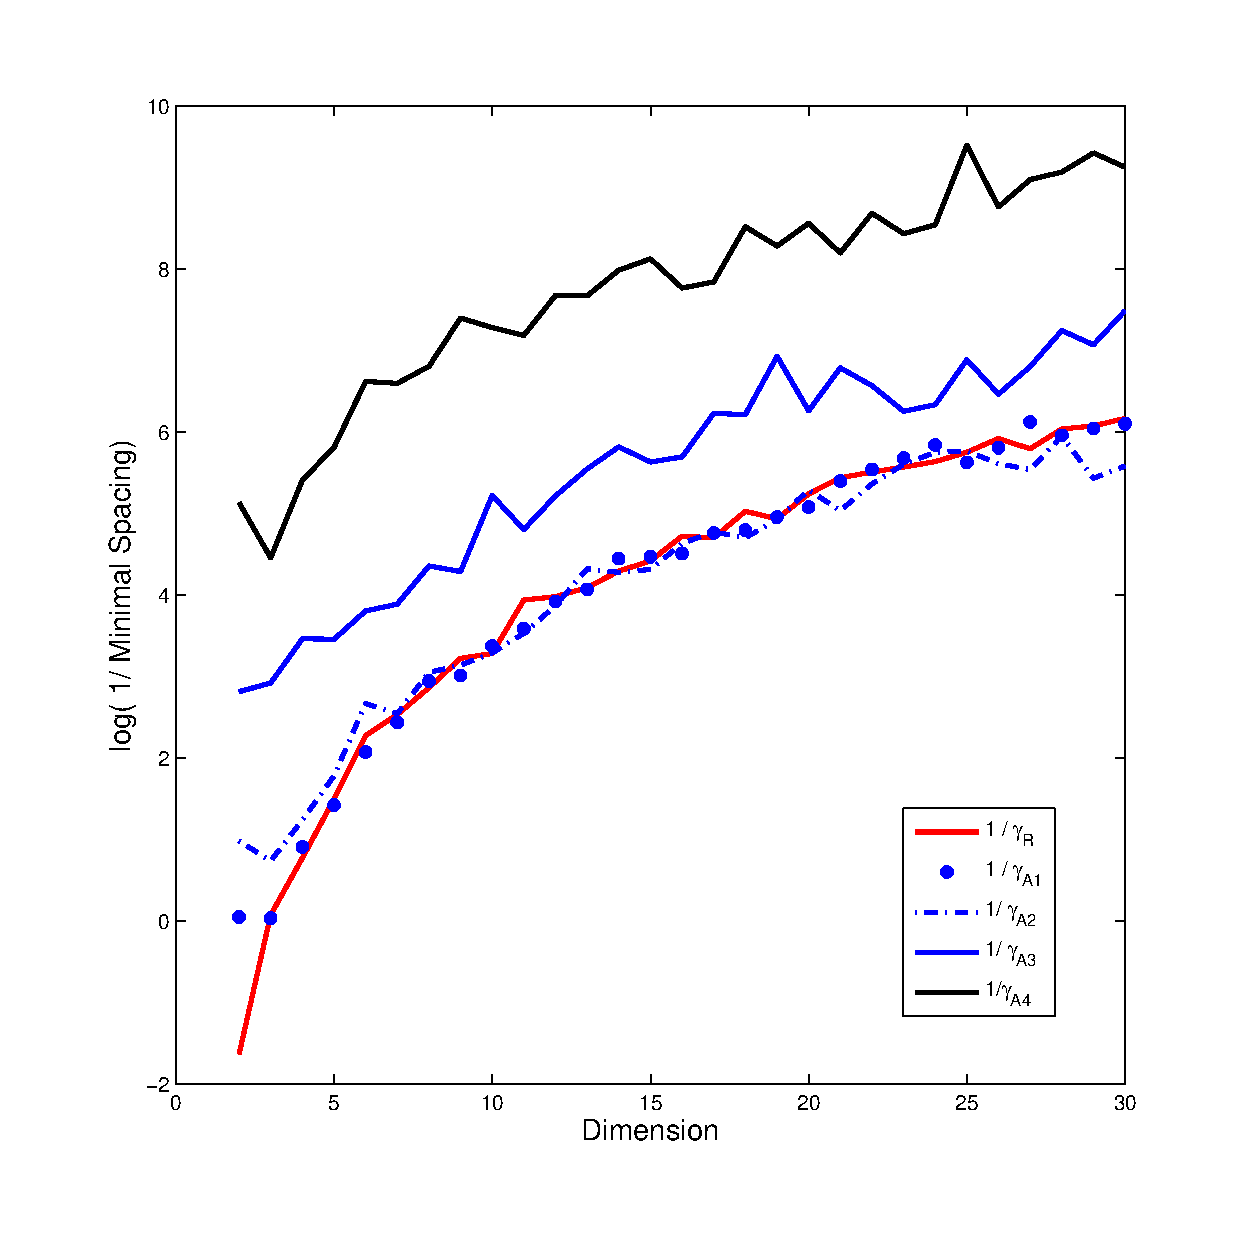
\includegraphics[width = 0.75\columnwidth]{miniSpacing}
%\vspace{-0.4cm}
\caption{
\label{fig:miniSpacing}
 The values of $1/\gamma$ for matrices with different coherences}
%\vspace{-0.5cm}
\end{figure}

%An empirical comparison of $1/\gamma_A$ and $1/\gamma_R$ is provided in Section~\ref{sec:gamma} in the appendix.
%\begin{remark}
% Note that all the conditions of Theorem~\ref{thm:Modefficiency} will be satisfied with probability 1 if $\xi$, $P(L_u)$, and $P\left(\frac{\sqrt{3}L_u}{\sqrt{2}\sigma_{\min}\kappa_{\min}^{1/2}C_1}\right)$  are small enough.

% Similarly, the result of Theorem~\ref{thm:Modefficiency} essentially depends on $\gamma_R$. 
% The main concern about Theorem~\ref{thm:Modefficiency} would be the behavior of this quantity. 
% Even though an analytic characterization of $\gamma_R$ is not yet known, a probabilistic lower bound for $\gamma_R$ can be developed (recall such lower bound is not available for $\gamma_A$) as shown in Section~\ref{subsec:gammaR}.
% Another two concerns would be: (1)When will these conditions hold? In particular, will these conditions hold in the traditional stochastic setting? (2)What is the probability of these events?
% We show that the answers to these questions are positive in Section \ref{subsec:gammaR} and \ref{subsec:ThminStocSetting}, which makes Theorem~\ref{thm:Modefficiency} meaningful. \qed
% \end{remark}
% \subsection{Behavior of $\gamma_R$}
% \label{subsec:gammaR}




To analyze $\gamma_R$ analytically,
note that $\phi_1$ and $\phi_2$ are independently sampled from the  standard Gaussian distribution. 
Thus, $\{\phi_1^{\top}R_1, \cdots, \phi_1^{\top}R_d,$ $\phi_2^{\top}R_1, \cdots, \phi_2^{\top}R_d\}$ are $2d$ independent standard Gaussian random variables. 
Let $Z_i = \frac{\phi_1^{\top}R_i}{\phi_2^{\top}R_i}$. Therefore, $Z_i$, $1\le i\le d$ are $d$ independent Cauchy$(0,1)$ random variables. Using this observation, we show in following lemma that $\gamma_R$ is large with probability at least $1-\delta$. Denote this event by $\EZ$.

\begin{proposition}
\label{prop:CauchyGap}
With probability at least $1-\delta$,
\[
\gamma_R \ge \frac{\delta(1-\delta/2)^{1/d}}{2(d-1)^2}.
\]
\end{proposition}

%Using this observation, we show in Lemma~\ref{lem:ConstantProb} in the appendix that, among others,  $\gamma_R \ge\frac{\delta}{2d^2}$ with probability at least $1-\delta$.

% We would need a high probability lower bound for $\gamma_R$
% %Recall that on the event $\Ephione$, $\min_i\vert Z_i \vert \ge \frac{\sqrt{2\pi}}{2d}$. 
% \begin{lemma}
% \label{lem:ConstantProb}
% With Probability at least $1-\delta$ , the following inequalities holds simultaneously.
% \begin{itemize}
% \vspace{-3mm}
% \item $\min_i |\psi^{\top}A_i| \ge \frac{\sqrt{\pi}A_{(2,\min)}}{5\sqrt{2}(d+1)} \delta$;
% \item $\min_i \{|\phi_2^{\top}R_i|\} \ge \frac{\sqrt{\pi}}{5\sqrt{2}(d+1)}\delta$;
% \item $\|\phi_1\|_2, \|\phi_2\|_2 \le \sqrt{2}\left(\sqrt{\log(\frac{5}{\delta})}+\sqrt{d}\right)$;
% \item $\gamma_R \ge\frac{\delta}{2d^2}$.
% \end{itemize}
% \vspace{-2mm}
% \end{lemma}
% Denote that above event by $\E$.
% \begin{remark}
% Note that all the constants in Lemma~\ref{lem:ConstantProb} are polynomial in $d$ (or $d^{-1}$ for the lower bound), thus the result of Theorem~\ref{thm:Modefficiency} is polynomial in $d$ and $\frac{1}{\delta}$ with probability at least $1-\delta$. \qed
% \end{remark}
Based on the above lemma, we show in the appendix that Theorem~\ref{thm:finalRes} holds for DICA.


\subsection{A Modified Version of DICA}
\label{subsec:modifiedDICA}
Furthermore, we provide a heuristic modification of DICA (MDICA) that performs better in the experiments (proving performance guarantees for that algorithm has defied our efforts so far). 
In practice, the estimation of the Hessian matrix introduces large estimation error.
The intuition of this modification is to reduce the number of estimating the Hessian matrix, while still keep the minimum spacing large.

%We would expect that DICA will achieve smaller error in the case of extreme coherence, since $1/\gamma_A$ will be much larger than $1/\gamma_R$. 
%However, the experimental results in Section~\ref{subsubsec:results} show the opposite.  
%The reason is that when the coherence is extremely high, the estimation error of $M$ in DICA is so much larger than that in HKICA that it dominates the error caused by the coherence of the mixing matrix.
%This estimation error comes from taking the inverse of $T_2$ in DICA. 
%Unfortunately, at the moment we don't understand well enough the relation of the estimation error and the coherence of the mixing matrix.

%We propose the following ICA algorithm, Algorithm \ref{alg:DICA_Mod}, trying to relieve the estimation error problem of DICA, but still keeping the large gap of the eigenvalues in the eigen-decomposition. 
\begin{algorithm} 
\caption{DICA Modified (MDICA)}
\label{alg:DICA_Mod}
\begin{algorithmic}[1]
\INPUT $x(t)$ for $1\le t \le T$. 
\OUTPUT An estimation of the mixing matrix $A$. 
\STATE Sample $\psi$ from a $d$-dimensional standard Gaussian distribution;
\STATE Evaluate $\nabla^2\hat{f}(\psi)$, \\
%\quad where $\hat{m_p}(\eta) = \frac{1}{T}\sum_{k=1}^{T} (\eta^{\top}g(k))^p$, and $\hat{f}(\eta) = \frac{1}{12}\big(\hat{m_4}(\eta) - 3\hat{m_2}(\eta)^2 \big)$;
\STATE Compute the SVD of $\nabla^2\hat{f}(\psi) = U \Sigma V^{\top}$, and let $\hat{B} =  U \Sigma^{1/2}$.
\STATE Sample $\phi$ from the standard normal distribution;
\STATE Compute $\hat{T} = \nabla^2 \hat{f}(\hat{B}^{-\top}\phi)$;
\STATE Compute all the eigenvectors of $\hat{M} = \hat{B}^{-1}\hat{T}\hat{B}^{-\top}$, $\hat{R} = \{\mu_1,\ldots,\mu_d\}$;
\STATE Return $\hat{A} = \hat{B}\hat{R}$.
\end{algorithmic}
\end{algorithm}
\begin{remark}
\label{rmk:DICA_Mod}
Note that the eigenvalues of $\hat{M}$ in MDICA are $\frac{(\phi^{\top}R_i)^2}{(\psi^{\top}A_i)^4\kappa_i}$ for $1\le i\le d$. 
When $A$ is highly coherent, we would expect that $\psi^{\top}A_i$'s are close to each other. 
%Also, the $\kappa_i$'s are fixed. 
Given that $\phi^{\top}R_i$'s are well separated from each other, we intuitively expect the eigenvalues to be well-separated from each other. 
However, we do not have a rigorous proof for this algorithm.
Experimental results show that MDICA consistently outperforms DICA. 

\end{remark}
%Note that the eigenvalues of the eigen-decomposition in MDICA are $\{ \frac{(\phi^{\top}R_i)^2}{(\psi^{\top}A_i)^4\kappa_i}\}$.
%Assume that $\kappa_i$ are all equal. 
The following proposition shows that the minimal spacing of $M$ in MDICA is large when $A$ is highly coherent. Instead of assuming the source function is bounded, we assume $\|A_i\|_2 = 1$.
\begin{proposition}
\label{prop:spacingMDICA}
For $0<\delta <1$, let $c = \frac{\sqrt{\pi/2}\delta}{(d-1)^2}$. Under the event of $\Epsi\cap\Ephi$, assume that
\begin{itemize}
%\item $L_u \ge |\psi^{\top}A_i| \ge \ell$ for any $1\le i\le d$;
%\item $| \phi^{\top}R_i - \phi^{\top}R_j| \ge c$ for any $1\le i\neq j \le d$;
%\item $|\phi^{\top}R_i| \ge q$ for any $1\le i\le d$;
\item $\kappa_i = \kappa$ for any $1\le i\le d$;
\item $<A_i, A_j> \,\ge 1-\eps$ for any $1\le i, j \le d$, such that $\eps \le \frac{\ell^4 c}{4L_u^3}$;
\end{itemize}
Then with probability at least $1-\delta$, the minimal spacing of $M$  in the MDICA algorithm is at least $\frac{\pi\delta\ell_l}{2\kappa L_u^4 (d-1)^2}$. 
\end{proposition}

\subsection{Recursive Versions}
Recently, \citet{vempala2014max} proposed a recursion idea to improve the sample complexity of the Fourier PCA algorithm of \citet{goyal2014fourier}. 
Instead of recovering all the columns of $A$ in a single eigen-decomposition, the recursive algorithm only decomposes the whole space into two subspaces according to the maximal spacing of the eigenvalues, 
then recursively decomposes each subspaces until they are all 1-dimensional.
The insight of this recursive procedure is the following: when the maximal spacing of the eigenvalues are much larger than the minimal one, the algorithm may win over a single decomposition even with the accumulating errors through the recursion.
However, this algorithm is based on the assumption that the mixing matrix is orthonormal, so that the projection to its subspaces can always eliminate some component of the source signal. 

We adapt the above idea to our algorithms. Due to space limit, we will only explain the simplest recursive algorithm, the recursive version of HKICA, as an example.

To force an orthonormal mixing matrix, we will first compute the square root matrix $B$ from $\nabla^2f(\psi) = AD_{\psi}KA^{\top}$ in the same way proposed in DICA. 
Thus $B = AD_{\psi}^{1/2}|K|^{1/2}R^{\top}$ for some orthonormal matrix $R$. 
Transforming our observations by $B^{-1}$, we then have the new observation $y(t) = B^{-1}x(t) + B^{-1}\eps(t) = RD_{\psi}^{1/2}|K|^{1/2}s(t) + B^{-1}\eps(t)$. 
Note that $B^{-1}\eps(t)$ is still a Gaussian noise. Also $D_{\psi}^{1/2}K^{1/2}$ is diagonal, thus $RD_{\psi}^{1/2}K^{1/2}s(t)$ is an orthonormal mixture of independent sources.
We then apply the recursive algorithm to recover the mixing matrix $R$. Finally, $BR$ gives an estimation of $A$ up to scaling.

To recover $R$ using a recursive algorithm, we follow the idea of HKICA (and DICA) to compute two Hessian matrices $T_1 = RD_{\psi}^{-1}\Lambda_1R^{\top}$ and $T_2 = RD_{\psi}^{-1}\Lambda_2R^{\top}$. 
Then, instead of computing the eigen-decomposition of $T_0=T_1 T_2^{-1}$ (as in HKICA), we only decompose its eigenspace into two subspaces, according to the maximal spacing of the eigenvalues of $T_0$. The \emph{Decompose} helper function takes a projection matrix $P$ of a subspace spanned
by some columns of $R$ (WLOG we assume it is the first $k$ columns of $R$). Then we compute the projection of $T_0$ as $M = P^{\top}T_0P$. Thus the eigenspace of $PMP^{\top}$ is in the span of $P$. 
Lastly, by separating the eigenvectors of $M$ according to its eigenvalues into $PP_1$ and $PP_2$, the Decompose function repeatedly decomposes the subspaces into two smaller subspaces.  

\begin{algorithm} 
\caption{Recursive version of HKICA (HKICA.R)}
\label{alg:HKICA_recur}
\begin{algorithmic}[1]
\INPUT $x(t)$ for $1\le t \le T$. 
\OUTPUT An estimation of the mixing matrix $A$. 
\STATE Sample $\psi$ from a $d$-dimensional standard Gaussian distribution;
\STATE Evaluate $\nabla^2\hat{f}(\psi) = \hat{G}(\psi)$; \\
\STATE Compute $\hat{B}$ such that $\nabla^2\hat{f}(\psi) = \hat{B}\hat{B}^{\top}$;
\STATE Compute $\hat{y}(t) = \hat{B}^{-1}x(t)$ for $1\le t \le T$;
\STATE Let $P = I_d$;
\STATE Compute $\hat{R} = \text{Decompose}(\hat{y}, P)$;
\STATE Return $\hat{B}\hat{R}$;
\end{algorithmic}
\end{algorithm}
\begin{algorithm} 
\caption{The Decompose helper function}
\label{alg:recur}
\begin{algorithmic}[1]
\INPUT $x(t)$ for $1\le t \le T$, a projection matrix $P\in \R^{d\times k}$ ($d\ge k$). 
\OUTPUT An estimation of the mixing matrix $A\in \R^{d\times k}$. 

\STATE if $k==1$, Return $P$;
\STATE Sample $\phi_1$ and $\phi_2$ independently from a standard Gaussian distribution of dimension $d$;
\STATE Evaluate $\nabla^2\hat{f}(\phi_1)$ and $\nabla^2\hat{f}(\phi_2)$, 
\STATE Compute $\hat{T} = (\nabla^2 \hat{f}(\phi_1))(\nabla^2\hat{f}(\phi_2))^{-1}$;
\STATE Compute $\hat{M} = P^{\top} \hat{T} P$;
\STATE Compute all the eigen-decomposition of $\hat{M}$, its eigenvalues$\{\sigma_1,\ldots,\sigma_d\}$ where $\sigma_1\ge\ldots\ge \sigma_k$ and their corresponding eigenvectors $\{\mu_1,\ldots, \mu_k\}$;
\STATE Find the index $m = \arg\max \sigma_m - \sigma_{m+1}$; 
\STATE Let $P_1 = (\mu_1,\ldots,\mu_m)$, and $P_2 = (\mu_{m+1},\ldots,\mu_k)$;
\STATE Compute $W_1 = \text{Recur} (x, PP_1)$, and  $W_2 = \text{Recur} (x, PP_2)$;
\STATE Return $[W_1,W_2]$;
\end{algorithmic}
\end{algorithm}

\begin{remark}
% Other algorithms can be modified to use a recursive estimation in a similar way, based on the idea of mapping the estimated Hessian matrix into a small subspace by $M = P^{\top}TP$. 
Other algorithms can be modified into a recursive version in a similar way. 
%\qed
\end{remark}
\begin{theorem}
\label{thm:recursiveAlg}
Given the conditions in Theorem~\ref{thm:finalRes}, with probability at least $1-\delta$, the recursive version of HKICA returns the mixing matrix with an error bound
\begin{align*}
& \quad \| \hat{A} - ADP\|_2 \\
\le & \poly{d,\frac{1}{\kappa_{\min}}, \frac{1}{\sigma_{\min}}, \frac{1}{\ell}, L_u, L, C, \sigma_{\max}}((\xi + P(L_u))^2 + \bar{\xi}).
\end{align*}
Here $D$ is some diagonal matrix and $P$ is some permutation matrix.
\end{theorem} 
\begin{remark}
Note that given large enough $T$, the term $(\xi + P(L_u))^2$ will be dominated by the error carried over from the quasi-whitening procedure, $\bar{\xi}$.
The recursion idea improves the sample complexity of the eigen-decomposition (to recover the orthonormal mixing matrix $R$).  
\end{remark}

\if0
\begin{remark}
In our result, the recursive version gets worse error bound, compared to the one-pass version. The reason is that the events $\Ephi$ and $\Ez$ could be required to hold for $d$ times. Therefore, for the final result to hold for probability at least $1-\delta$, the error bound for each recursion has to hold with probability at least $1-\frac{1}{d}\delta$. 

Recall that in our case we have lower bound for the minimal eigenvalue spacing as $O(\frac{1}{d^2}\delta)$, and lower bound for maximal eigenvalue spacing as $O(\frac{1}{d}\delta)$. By requiring it holds for higher probability ($1-\frac{1}{d}\delta$), the maximal gap actually reduced to $O(\frac{1}{d^2}\delta)$, same order as the one-pass version, leading to the same error bound.

Moreover, for the event $E\phi$, the recursive version essentially require the lower bound $\ell$ is $d$ times smaller than the one-pass version, which cause high degrees of $d$ in the error bound.

For the recursive version to help, one possible way is to prove that for each recursion, we only require the conclusion holds with probability at least $1-\frac{1}{\log d}\delta$, rather than $1-\frac{1}{d}\delta$. 
Another potential improvement is developing a lower bound for the maximal spacing that is sub-polynomial in $d$, e.g. $\frac{1}{\log d}\delta$, and sub-polynomial dependence of $\delta$ in the lower bound in the Event $\Ephi$, e.g. $\frac{1}{\log \frac{1}{\delta}}$.    
\qed
\end{remark}
\fi
\section{Experimental Results}
\label{sec:ExpRes}
In this section we compare the performance of different ICA algorithms
in some synthetic examples, with mixing matrices of different coherences.

% For each of the matrices, we generate $\phi$ and $\psi$ from standard normal distribution for 3 times, and pick the minimal values (corresponding to the largest $\gamma_A$ and $\gamma_R$).
% We run 200 repetitions and take the average of each $1/\gamma$. The logarithm of the average is reported in Figure~\ref{fig:miniSpacing}.
% \begin{figure}[h]
% \label{fig:miniSpacing}
% \centering
% 	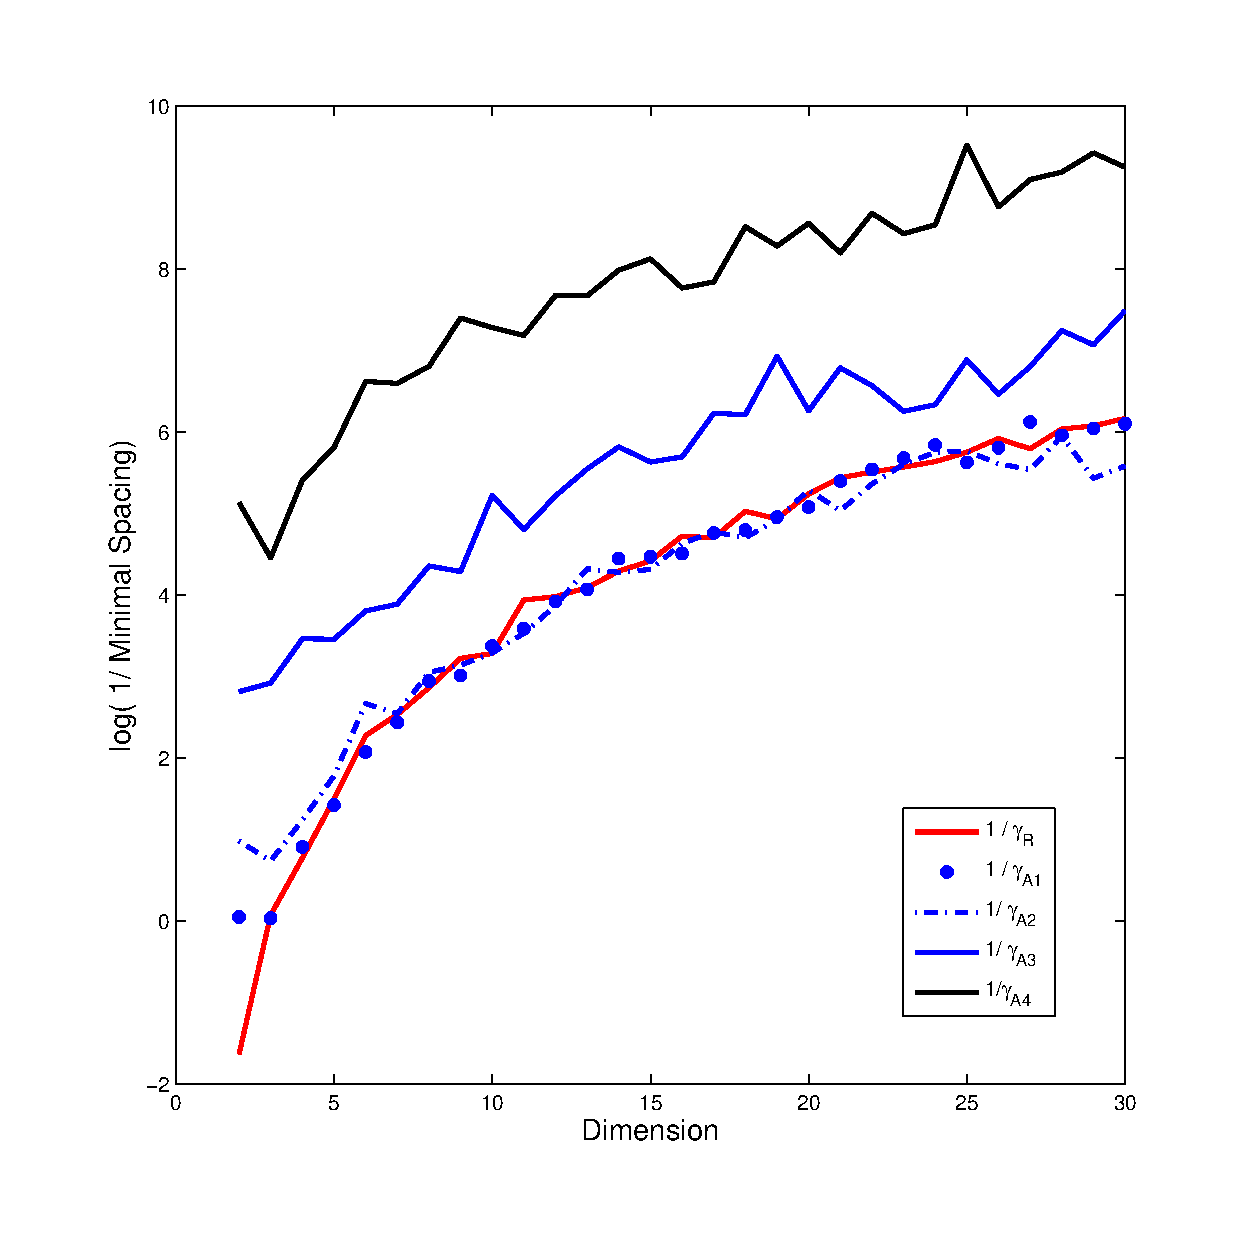
\includegraphics[width = \columnwidth]{miniSpacing}
% \caption{The values of $\gamma$ for matrices with different coherences}
% \end{figure}


We test 9 algorithms: 
HKICA (HKICA), and its recursive version (HKICA.R); 
DICA  (DICA), and its recursive version (DICA.R);  
the modified version of  DICA  (MDICA), and its recursive version (MDICA.R);
the default FastICA algorithm from the 'ITE' toolbox \citep{szabo12separation} (FICA);
the recursive Fourier PCA algorithm of \citet{xiao2014FPCAPackage} (FPCA);
and random guessing (Random).
FPCA is modified so that it can be applied to the case of non-orthogonal mixing matrix.
%\item Symmetrizing version of  HKICA  (HKICA\_Symm), and its recursive version (HKICA\_Symm\_recur);
%\item Symmetrizing version of  DICA  (DICA\_Symm), and its recursive version (DICA\_Symm\_recur);
%Recall that the re-sampling version and the symmetrizing version are two different ways for the algorithms to deal with complex (invalid) output, as discussed in Remark \ref{rmk:symmetrization}.
%FastICA, as one of the most popular ICA algorithm in the literature, is evaluated and reported as a baseline. 
%We will discuss the intuition of the DICA\_Int algorithm later. 
%We include the Fourier PCA algorithm as another baseline, with a moderately tuned parameter. 
%The random guessing algorithm, which returns a randomly guessing matrix, serves as the last baseline.
%We do not test the algorithm of \citep{anandkumar2012tensordecomposition} because the tensor decomposition takes too long to converge and achieve a valid solution. 

In the simulation, a common mixing matrix $A$ of dimension 6 is generated in the following ways:
We construct four kinds of matrices:
$A_1 = P$; 
$A_2 = v_b\times\boldsymbol{1}^{\top} + 0.3\times P$;
$A_3 = v_b\times\boldsymbol{1}^{\top} + 0.05\times P$;
and $A_4 = v_b\times\boldsymbol{1}^{\top} + 0.005\times P$.
Here the vector $v_b$ and the matrix $P$ are both generated from standard Gaussian distribution (with different dimensions).
We also generate an orthonormal mixing matrix R, obtained by computing the left column space of a non-singular random matrix (from standard normal distribution).  
Then we generate a $6$-dimensional BPSK signal $s$ as follows. Let $p=(\sqrt{2},\sqrt{5},\sqrt{7},\sqrt{11},\sqrt{13},\sqrt{19})$.
We generate a $\{+1,-1\}$ valued sequence $q(t)$ uniformly at random for $1 \le t \le T$, and set
$s_i(t) = q(t) i\times\sin (p_i t)$.
Note that in order to have the components of $s$ close to independent, we need the ratio of their frequencies to be irrational. 

Lastly, the observed signal is generated as $x = As+c\epsilon$ where $\epsilon$ is the noise generated from a $d$-dimensional normal distribution with randomly generated covariance. 
We take $T=20000$ instances of the observed signal on time steps $t= 1,\ldots, 20000$.
We test the noise ratio $c$ from 0 (noise-free) to 1 (heavily noisy). 
All the algorithms are evaluated on a $150$ repetitions. 
Since the algorithms are randomized, for each repetition we try $3$ times and report the best.

We measure the performances of the algorithms by its actual reconstruction error.
In particular, we evaluate the following quantity between the true mixing matrix $A$ and the estimate $\hat{A}$ returned by the algorithms:
\begin{equation}
\label{equ:parerror}
\min_{\Pi,S} \|\hat{A}\Pi S - A\|_{\text{Frob}},
\end{equation}
where $\Pi$ is a permutation matrix, and $S$ is a column scaling matrix (diagonal).
The calculation of this measure requires an exhaust search for the optimal permutation.

\if0
The second measure we used is an approximation of Equation \eqref{equ:parerror} proposed by \citet{comon1994independent}. 
Note that to evaluate Equation \eqref{equ:parerror} one has to enumerate all the permutation $\Pi$, which is not affordable in practice for a large dimension $d$. 
This error helps avoid this computation problem. 

The last measure is the mutual information between the joint distribution of the recovered sources and the product of its marginal ones. 
This measure is common in practice when the true mixing matrix $A$ is unknown. 
In fact, this measure can be reduced to the sum of the entropies of its marginal distribution \citep{Learned-Miller:2003:IUS:945365.964306}. 
In particular for an output $\hat{A}$, we evaluate the following quantity:
\begin{equation}
\sum_{i = 1}^{d} \text{Entropy}(\hat{x_i}) + \log |\hat{A}|,
\end{equation}
where $\hat{x} = \hat{A}^{-1}y$, and $|\hat{A}|$ is the absolute value of the determine of $\hat{A}$. We also use the entropy estimation function 'HShannon\_kNN\_k\_estimation' in the 'ITE' toolbox \citep{szabo14information}. 
\fi

\subsection{Results}
\label{subsubsec:results}
We report the reconstruction errors for different kinds of mixing matrices and noise ratios.

\begin{figure}[t] %pt]
	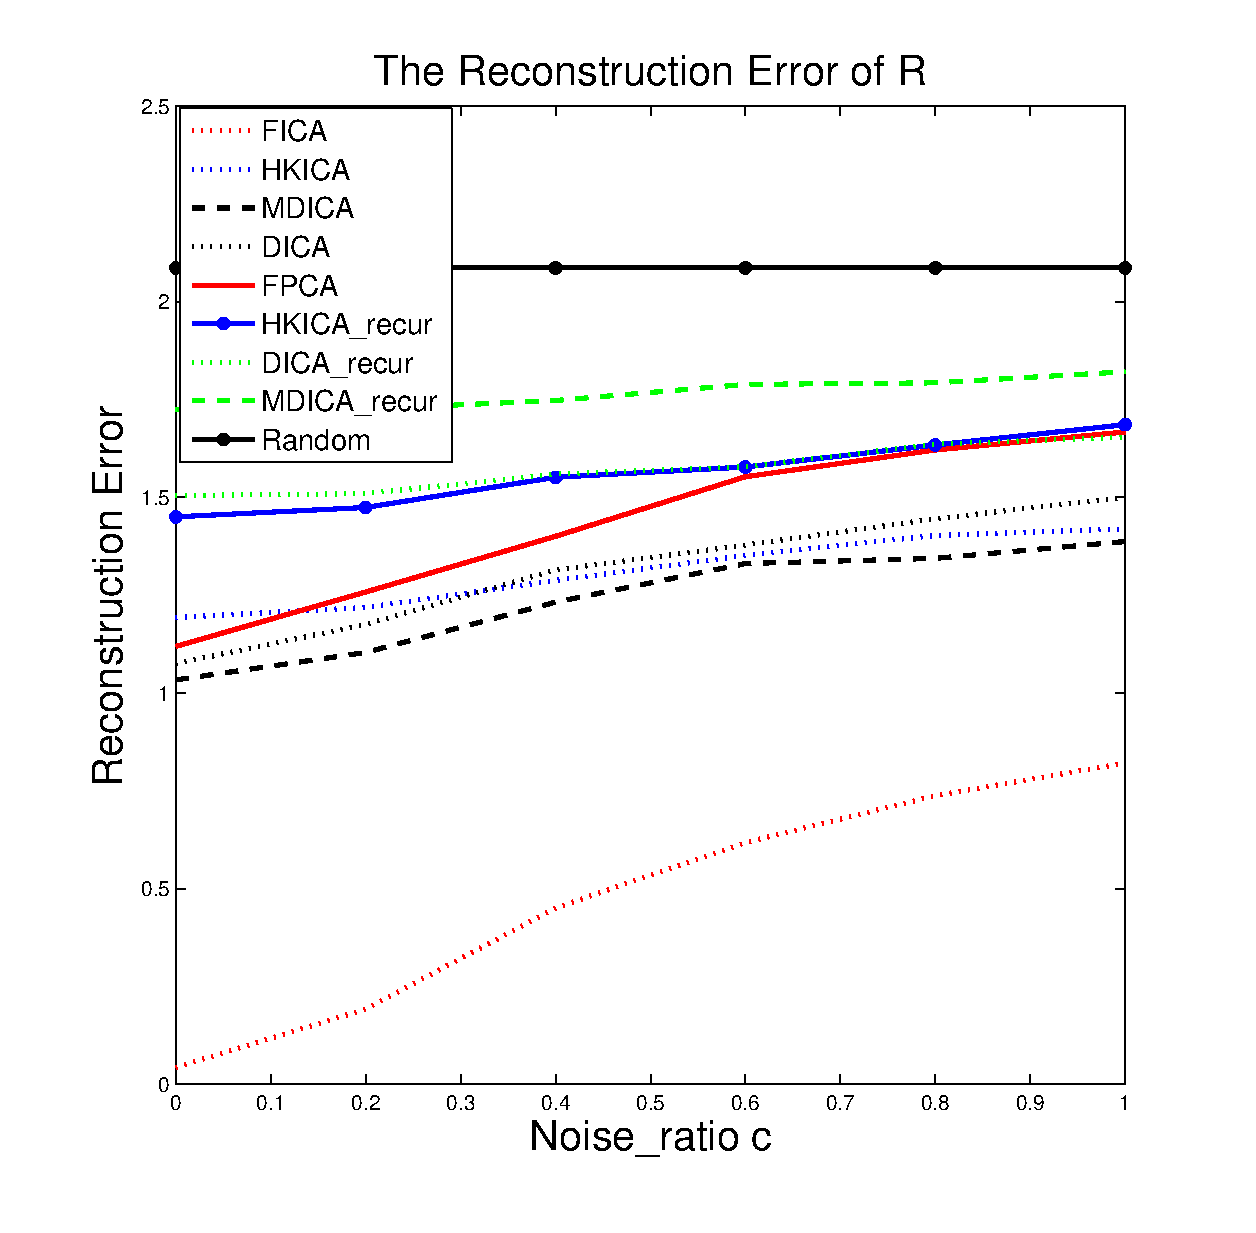
\includegraphics[width =0.45\columnwidth]{errorR}
	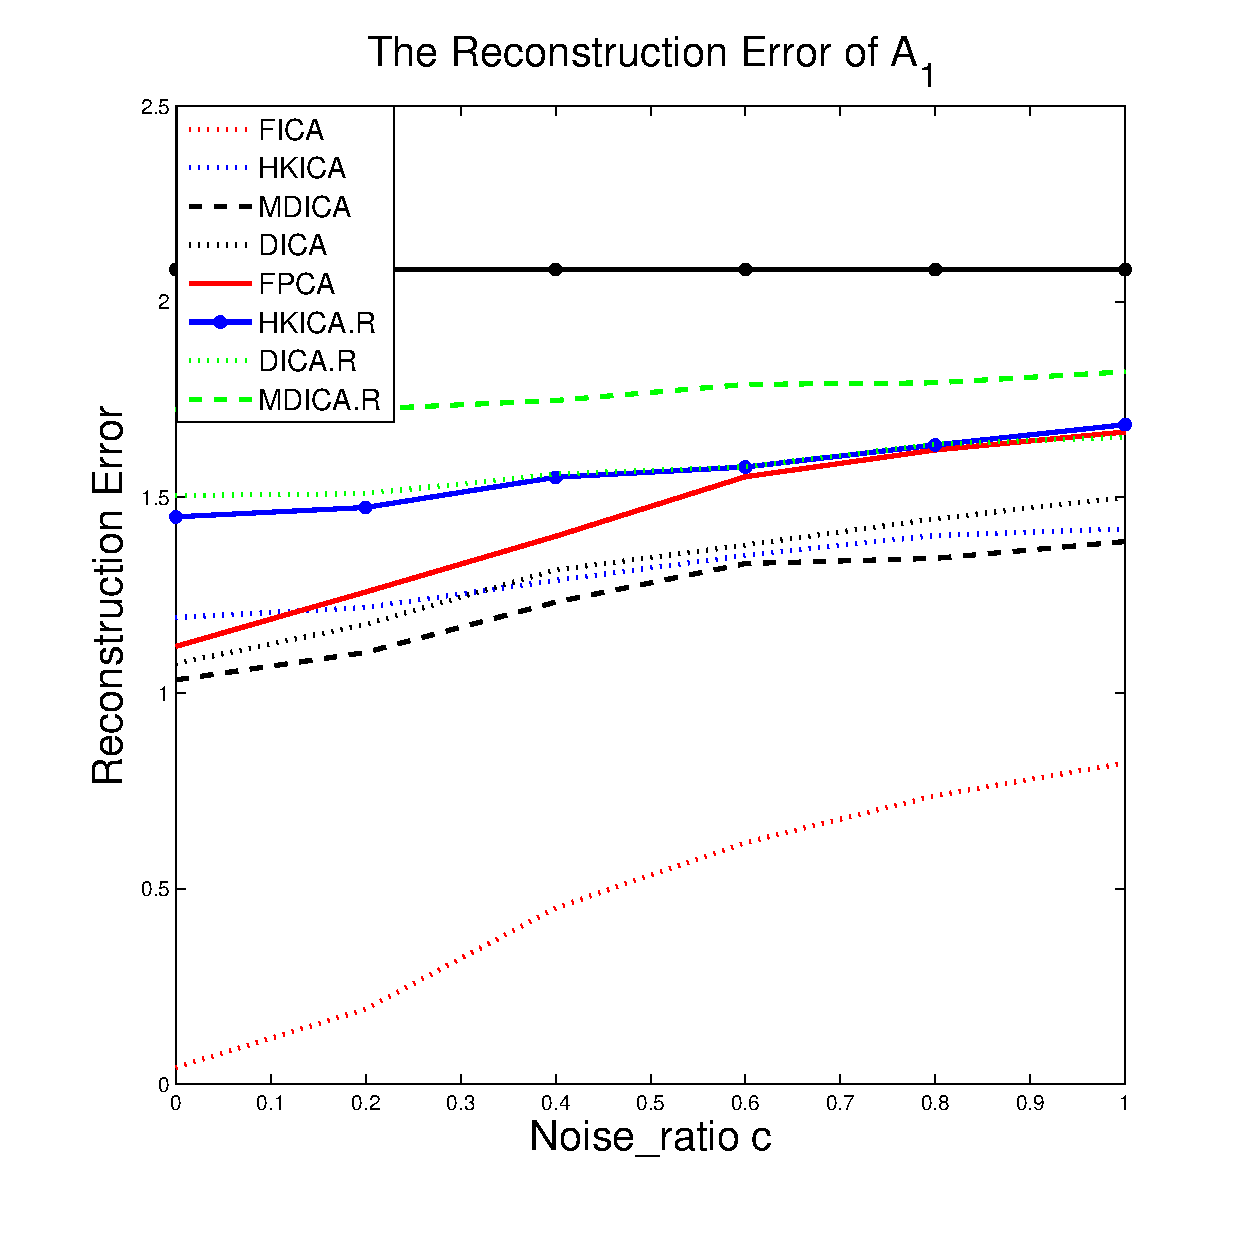
\includegraphics[width =0.45\columnwidth]{error1} \\
	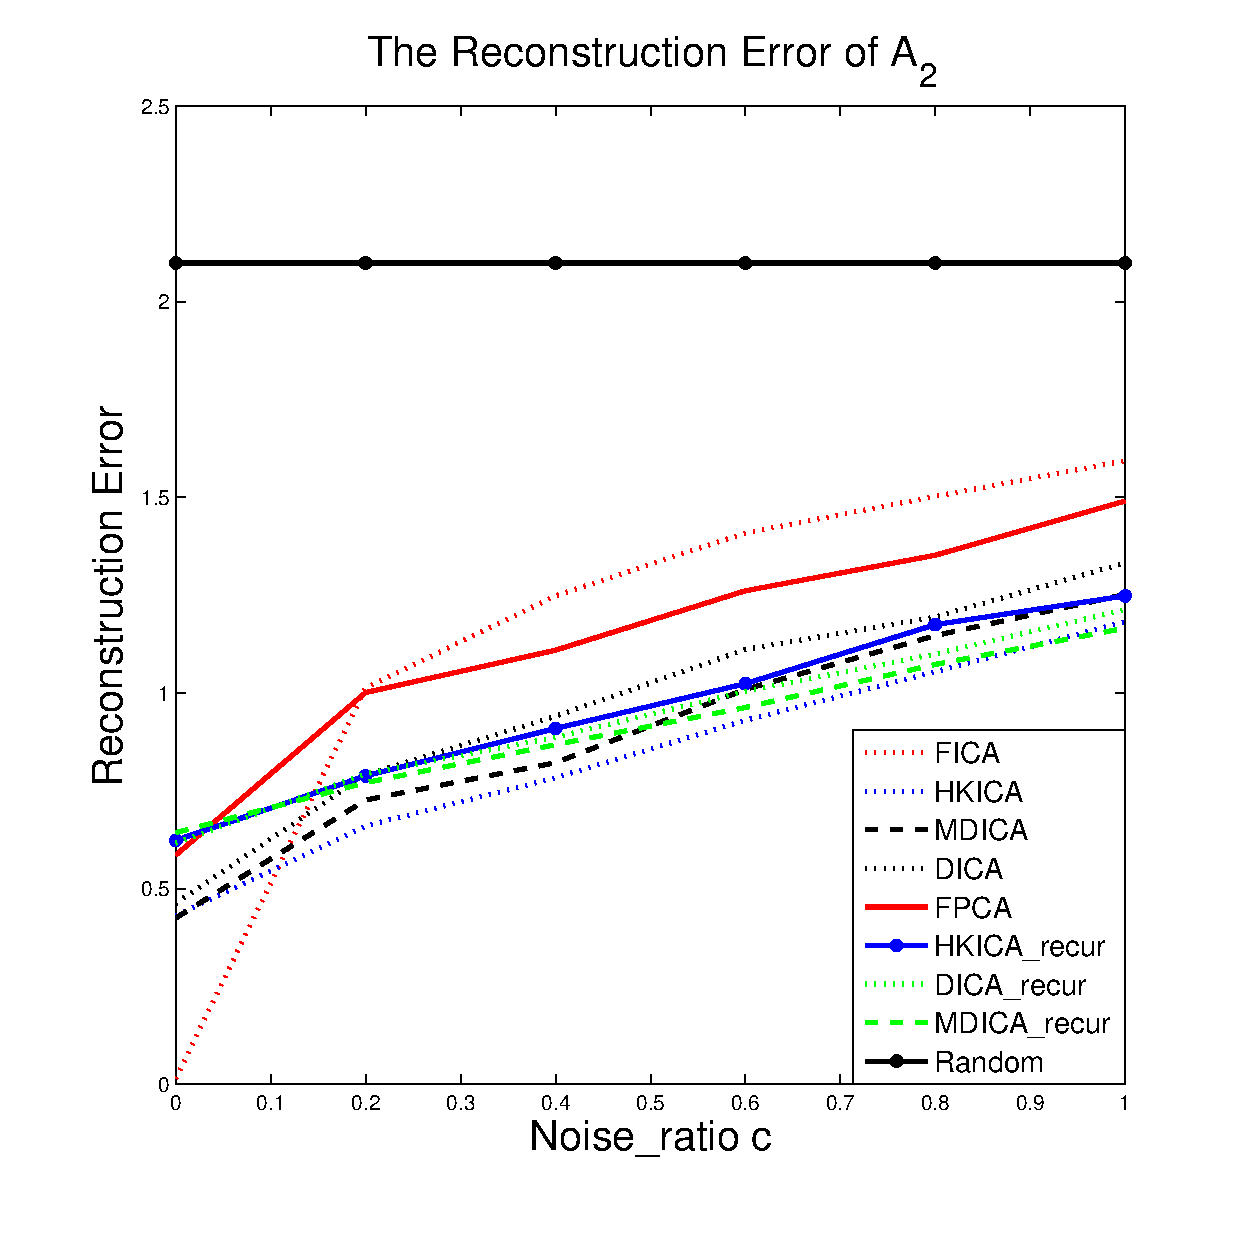
\includegraphics[width =0.45\columnwidth]{error2}
	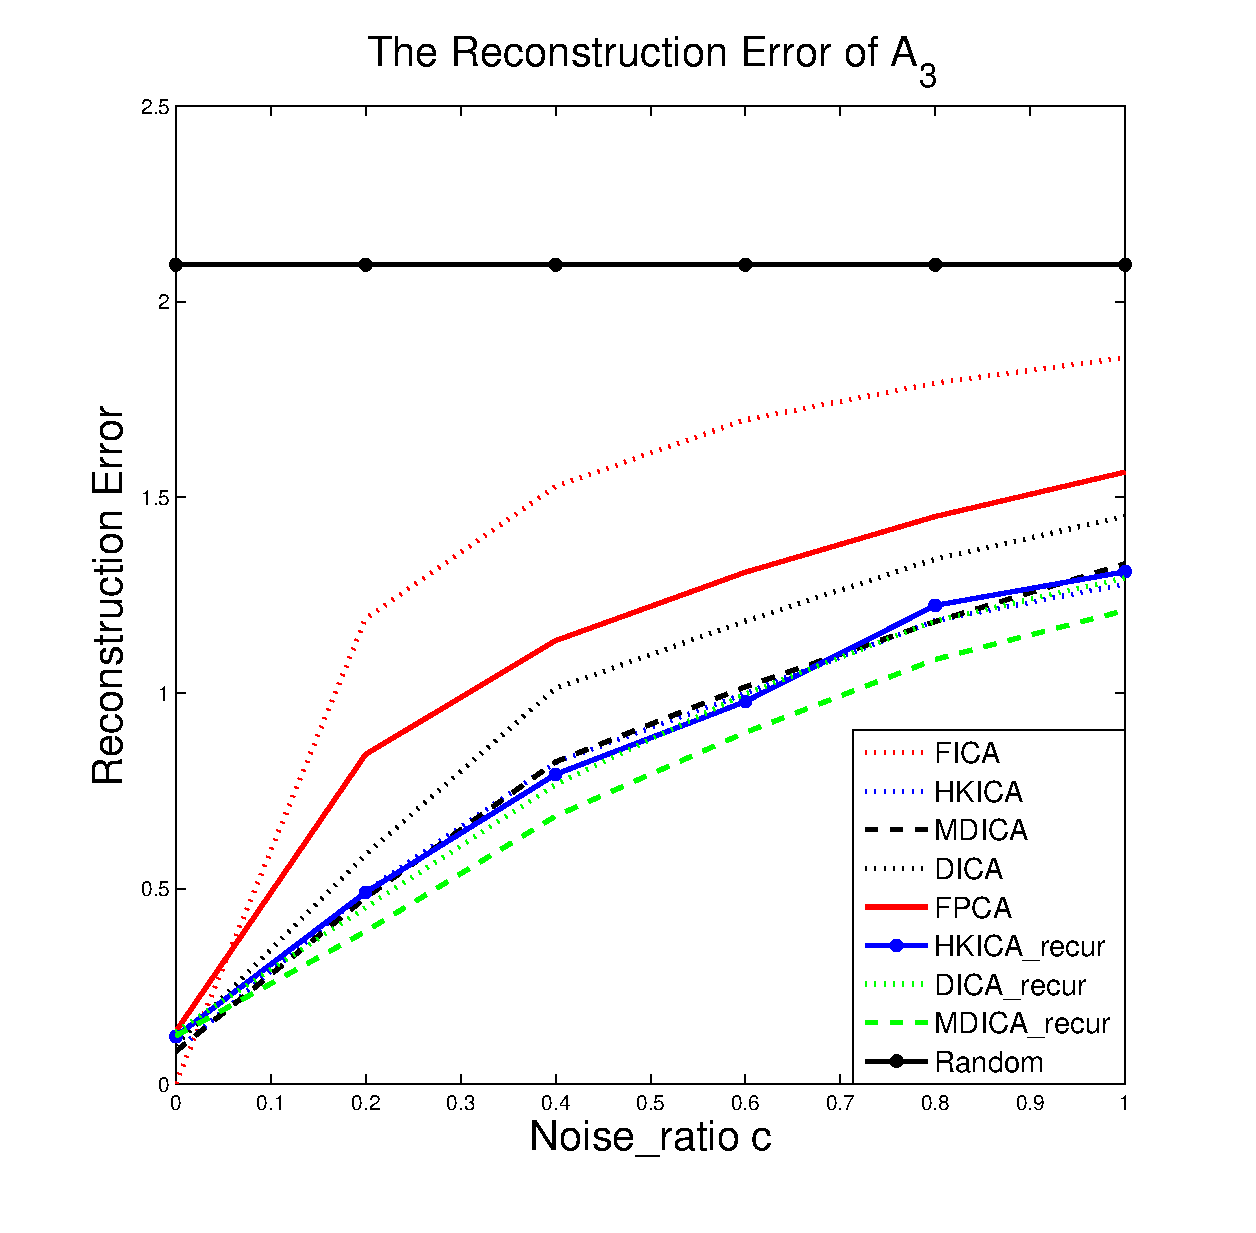
\includegraphics[width =0.45\columnwidth]{error3} \\
	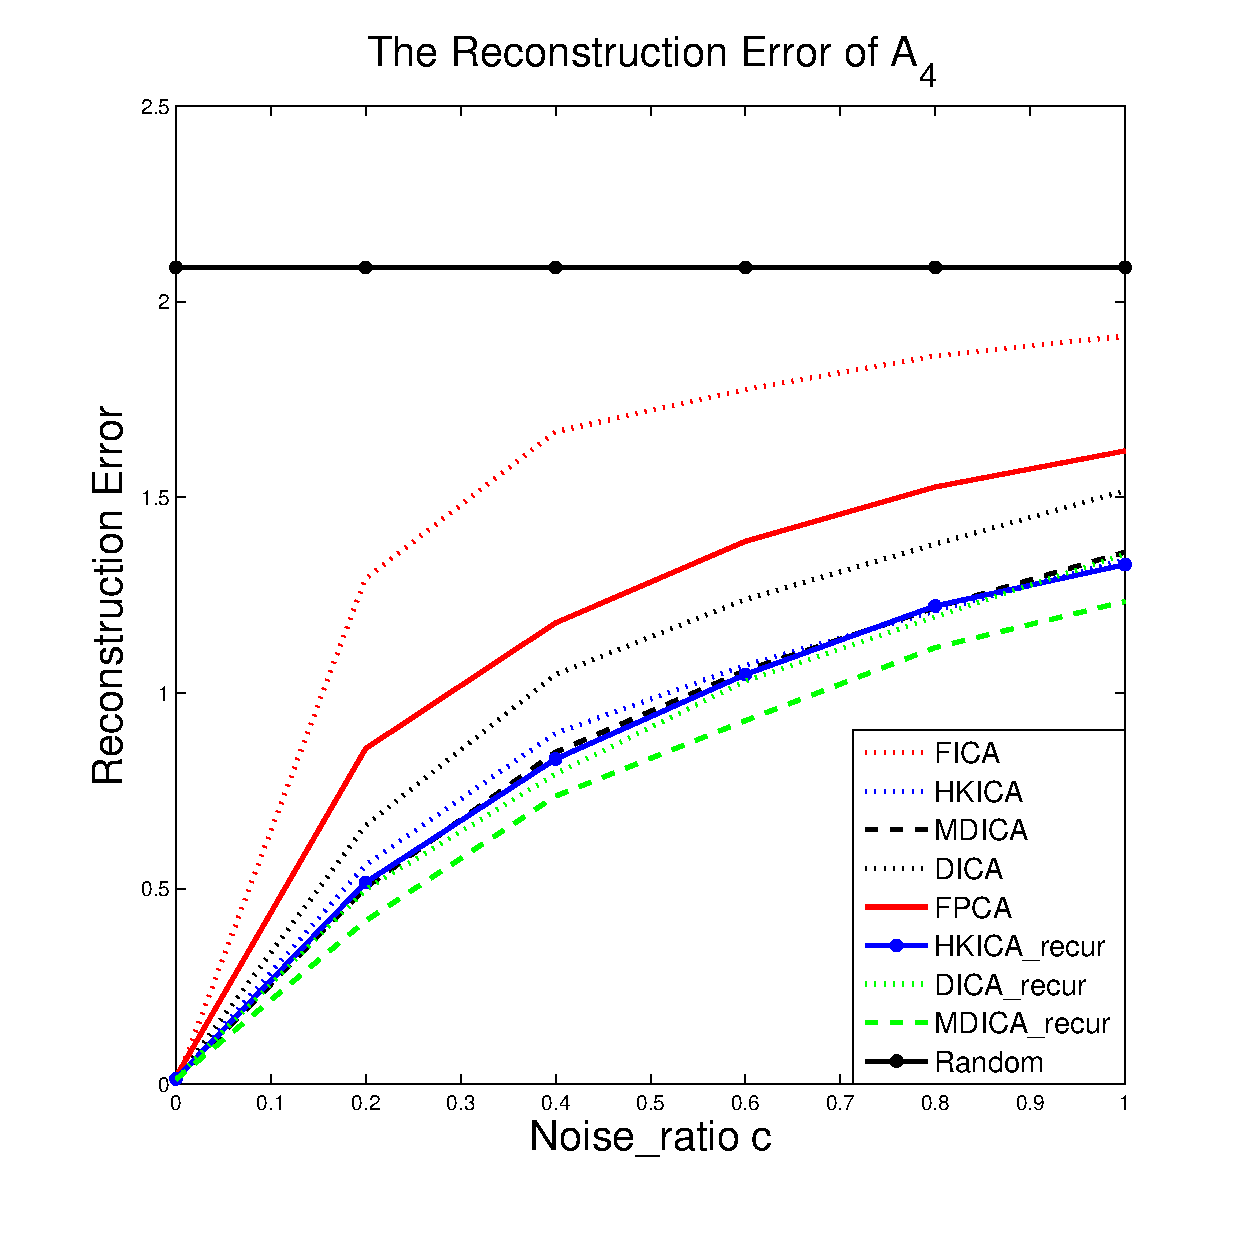
\includegraphics[width =0.45\columnwidth]{error4}
\vspace{-0.5cm}
\caption{
\label{fig:Error}
 Reconstruction Errors}
\end{figure}
The experimental results suggest that moment methods are more robust
to high-coherence mixing matrices and Gaussian noise than FastICA.
FastICA achieves the best performance in case of low coherence.
As the coherence of the mixing matrix $A$ increases, its performance decreases quickly and becomes sensitive to noise. 

We expected that DICA will achieve smaller error for an extremely coherent $A$, since $1/\gamma_A$ will be much larger than $1/\gamma_R$. 
However, the experimental results indicate the opposite. 
Note that high coherence implies small minimal singular value.
In this case, the estimation error of $M$ in DICA could be much larger than that in HKICA, because of the fourth degree of $A^{-1}$.
%Also DICA requires estimation of more fourth moments. 
This error overwhelms the improvement brought by larger eigenvalue
spacings, if the sample size is not large enough.
The investigation of this phenomenon is left for future work.
%Due to the time limit, we haven't confirm this argument by more experiments yet.

On the other hand, MDICA tries to achieve a small estimation error, meanwhile we expect it to keep the eigenvalue spacing large
(intuitively, it is approximately the spacing of the square of $d$ Gaussian random variables), leading to good performance.
This is confirmed by the experimental results, in both the non-recursive and recursive versions.

The recursive idea is not always helpful for the moment methods. For a highly coherent $A$, the recursive versions outperform their non-recursive counterparts.
Note that in this case, $A$ is close to singular (small minimal
singular value), and thus it requires more samples.
On the other hand, when $A$ has relatively low coherence,  the estimation error of the fourth moments contributes more to the reconstruction error. 
Recursive algorithms suffers from making several such estimations.

In summary, the results suggest that these moment methods are comparable to each other in practice,
while FastICA  is better for mixing matrices with low coherence or mild coherence with low noise.
If the mixing matrix is orthonormal, then FPCA performs better than
the other algorithms.
If the observations have heavy noise and the mixing matrix is not extremely coherent, then HKICA may be the best choice.
In the case of an extremely coherent mixing matrix, MDICA performs the
best. Also, the recursive idea is very helpful for small sample sizes.

\section{Conclusions}
We considered the problem of independent component analysis with noisy
observation. For the first time in the literature, we presented ICA algorithms that can recover non-Gaussian
source signals with polynomial computational complexity and provable performance guarantees on the reconstruction
error that guarantee that for $T$ samples the reconstruction error
vanishes at a $1/\sqrt{T}$ rate and depends only polynomially on the
natural parameters of the problem. The algorithms do not depend on
unknown problem parameters, and also extend to deterministic sources
with approximately independent empirical distributions.


\subsection*{Acknowledgements}

This work was supported by the Alberta Innovates Technology Futures
%through the Alberta Innovates Centre for Machine Learning 
and NSERC.

\newpage 
\bibliography{DICA}
%\bibliographystyle{plainnat}

%!TEX root =  DICA.tex
\onecolumn

\section{Appendix}
\label{sec:Appendix}

\subsection{Proof of Proposition \ref{prop:stochasticAss}}
Denote the population expectation by $\E$ and the empirical expectation by $\E_t$. We restate the assumptions here.
\begin{enumerate}[(i).]
\vspace{-3mm}
\item $\| \E_t[S] \|_F\le L/\sqrt{t}$;
\item $\| \E_t[\epsilon] \|_F \le L/\sqrt{t}$;
\item $\| \E_t[\epsilon^{\otimes 2}] \|_F \le L$;
\item $\| \E_t[\epsilon^{\otimes 3}] \|_F \le L$;
\item $\| \left(\E_{Y\sim \nu_t^{(\epsilon)}} [Y^{\otimes4}] - (\E_{Y\sim \nu_t^{(\epsilon)}} [Y^{\otimes2}])^{\otimes 2}\right)(\eta,\eta,\cdot,\cdot)  - 2 (\E_{Y\sim \nu_t^{(\epsilon)}} [Y^{\otimes2}])^{\otimes 2}(\eta,\cdot,\eta,\cdot)\|_F\le L/\sqrt{t} \|\eta\|_2^2$;
\item for $i_1,i_2,j_1,j_2 \ge 0$ that $i_1+i_2+j_1+j_2 \le 4$,  
\begin{align*}
\| \E_t[(AS)^{\otimes i_1} \otimes \E_t[\epsilon^{\otimes j_1}] \otimes (AS)^{\otimes i_2}] - \E_t[(AS)^{\otimes i_1}\otimes \epsilon^{\otimes j_1}\otimes (AS)^{\otimes i_2}]  \|_F \le L/\sqrt{t},
\end{align*}
and 
\begin{align*}
\| \E_t[\epsilon^{\otimes j_1} \otimes \E_t[(AS)^{\otimes i_1}] \otimes \epsilon^{\otimes j_2}] - \E_t[ \epsilon^{\otimes j_1}\otimes (AS)^{\otimes i_1}\otimes \epsilon^{\otimes j_2}]  \|_F \le L/\sqrt{t}.
\end{align*}
\end{enumerate}
Since $s$ is bounded by $C$, the first assumption will be satisfied with high probability $1-\delta$ by picking $L = C\sqrt{2d\log(\frac{1}{\delta})}$ by Hoeffding's inequality. Assumption (ii) to (v) are all about the moments of the Gaussian noise. 
For i.i.d. standard Gaussian random variables, $X_1, \ldots, X_t$, note that
\begin{itemize}
\item $ \E[\sum_j X_j/t] = 0$, $\text{Var}(\sum_j X_j/t) = 1/t$;
\item $ \E[\sum_j X_j^2/t] = 1$, $\text{Var}(\sum_j X_j^2/t) = 2/t$;
\item $ \E[\sum_j X_j^3/t] = 0$, $\text{Var}(\sum_j X_j^3/t) = 15/t$;
\item $ \E[\sum_j X_j^4/t] = 3$, $\text{Var}(\sum_j X_j^4/t) = 96/t$.
\end{itemize}
Therefore, by Chebyshev's inequality,
\begin{itemize}
\item with probability at least $1-\delta$, $|\sum_j X_j/t| \le \sqrt{1/t\delta}$;
\item with probability at least $1-\delta$, $|\sum_j X_j^2/t -1 | \le \sqrt{2/t\delta}$;
\item with probability at least $1-\delta$, $|\sum_j X_j^3/t| \le \sqrt{15/t\delta}$;
\item with probability at least $1-\delta$, $|\sum_j X_j^4/t -3| \le \sqrt{96/t\delta}$;
\end{itemize}
Given $\epsilon \sim \mathcal{N}(0,\Sigma)$ for some fixed unknown $\Sigma$, firstly consider the case when $\Sigma = I$.
Consider the $i$th entry of the 1-dimensional tensor (vector), with probability at least $1-\delta$, 
\[
\left| \sum_j \eps_i(j)/t \right| \le \sqrt{1/t\delta}.
\]
Thus, with probability at least $1-d\delta$,
\[
\| \sum_j \eps(j)/t \|_F \le \sqrt{d/t\delta}.
\]
For (iii), consider the position $(u,v)$ of the 2-dimensional tensor (matrix). If $u=v$ with probability at least $1-\delta$,
\[
	\left| \sum_j \eps_u^2(j)/t - 1\right| \le \sqrt{2/t\delta}.
\]
If $u\neq v$, by Chebysev's inequality with probability at least $1-\delta$,
\[
	\left| \sum_j \eps_u(j)\eps_v(j)/t \right| \le  \sqrt{1/t\delta}.
\]
Therefore, with probability at least $1-d^2\delta$, all entries are less that $1+\sqrt{2/t\delta}$. Thus 
\[
\|\E_t[\epsilon^{\otimes 2}]\|_F \le d(1+\sqrt{2/t\delta}).
\]
Similarly for (iv), consider the $(u,v,w)$ position for different cases. The expectation of $\eps_u\eps_v\eps_w$ is 0 and its variance is at most  $15$. Therefore, with probability at least $1-\delta$,
\[
\left|\sum_j \eps_u(j)\eps_v(j)\eps_w(j)/t \right| \le \sqrt{15/t\delta}.
\]
Thus, with probability at least $1-d^3\delta$,
\[
\|\E_t[\epsilon^{\otimes 3}]\|_F \le \sqrt{15d^3/t\delta}.
\] 
Lastly for (iv), each of the following inequalities holds with probability at least $1-\delta$,
\begin{align*}
& \left| \sum_j\eps_u^4(j)/t -3 \right| \le \sqrt{96/t\delta}; \quad \left| \sum_j\eps_u^3(j)\eps_v(j)/t \right| \le \sqrt{15/t\delta}; \quad \left| \sum_j\eps_u^2(j)\eps_v^2(j)/t - 1\right| \le \sqrt{4/t\delta}; \\
&  \left| \sum_j\eps_u^2(j)\eps_v(j)\eps_w(j)/t \right| \le \sqrt{2/t\delta}; \quad \left| \sum_j\eps_u(j)\eps_v(j)\eps_w(j)\eps_z(j)/t \right| \le \sqrt{1/t\delta};
\end{align*}
Consider the $(u,v)$ position of the matrix,
\begin{align*}
& \quad \left|\left(\E_t[\epsilon^{\otimes4}](\eta,\eta,\cdot,\cdot) - (\E_t[\epsilon^{\otimes2}])^{\otimes 2}(\eta,\eta,\cdot,\cdot) - 2(\E_t[\epsilon^{\otimes2}])^{\otimes 2}(\eta,\cdot,\eta,\cdot) \right)_{u,v}\right|\\
& \le \left| \left(\sum_j \eps_u(j)\eps_v(j)\sum_{k_1}\eta_{k_1}\eps_{k_1}(j)\sum_{k_2}\eta_{k_2}\eps_{k_2}(j)\right)/t- \E\left[ \eps_{u}\eps_{v}\sum_{k_1}\eta_{k_1}\eps_{k_1}\sum_{k_2}\eta_{k_2}\eps_{k_2}\right]\right| \\ 
& \quad + \left| \left(\sum_j \eps_u(j)\eps_v(j)\right)/t -  \E\left[ \eps_{u}\eps_{v}\right]\right|\left|\left(\sum_j\sum_{k_1}\eta_{k_1}\eps_{k_1}(j)\sum_{k_2}\eta_{k_2}\eps_{k_2}(j)\right)/t \right| \\
& \quad + 2\left| \left(\sum_j \eps_u(j)\sum_{k_1}\eta_{k_1}\eps_{k_1}(j)\right)/t\left(\sum_j \eps_v(j)\sum_{k_2}\eta_{k_2}\eps_{k_2}(j)\right)/t- \E\left[ \eps_{u}\sum_{k_1}\eta_{k_1}\eps_{k_1}\right]\E\left[\eps_{v}\sum_{k_2}\eta_{k_2}\eps_{k_2}\right]\right| 
\end{align*}
Note that the above inequality including $3d^2$ terms of concentration equations. Thus, with probability at least $1-3d^2\delta$,
\[
\left|\left(\E_t[\epsilon^{\otimes4}](\eta,\eta,\cdot,\cdot) - (\E_t[\epsilon^{\otimes2}])^{\otimes 2}(\eta,\eta,\cdot,\cdot) - 2(\E_t[\epsilon^{\otimes2}])^{\otimes 2}(\eta,\cdot,\eta,\cdot) \right)_{u,v}\right| 
\le
4\sqrt{15/t\delta}(1+\sqrt{2/t\delta})d\|\eta\|^2_2.  
\]
Thus, 
\[
\| \left(\E_{Y\sim \nu_t^{(\epsilon)}} [Y^{\otimes4}] - (\E_{Y\sim \nu_t^{(\epsilon)}} [Y^{\otimes2}])^{\otimes 2}\right)(\eta,\eta,\cdot,\cdot)  - 2 (\E_{Y\sim \nu_t^{(\epsilon)}} [Y^{\otimes2}])^{\otimes 2}(\eta,\cdot,\eta,\cdot)\|_F \le 4\sqrt{15/t\delta}(1+\sqrt{2/t\delta})d^2\|\eta\|^2_2.
\]
\if0
For the position $(i_1,i_2,i_3,i_4)$ of the tensor $\E_t[\epsilon^{\otimes4}] - 3(\E_t[\epsilon^{\otimes2}])^{\otimes 2}$ is
\[
\sum_j \eps_{i_1}(j)\eps_{i_2}(j)\eps_{i_3}(j)\eps_{i_4}(j)/t - 3(\sum_j \eps_{i_1}(j)\eps_{i_2}(j)/t)(\sum_j \eps_{i_3}(j)\eps_{i_4}(j)/t) = \sum_j \eps_i(t)^4/t - 3(\sum_j \eps_i(t)^2/t)^2  - \E[\eps_i^4] + 3(\E[\eps_i^2])^2.
\]  
Thus, 
\begin{align*}
|\sum_j \eps_i(t)^4/t - 3(\sum_j \eps_i(t)^2/t)^2| & \le \left|\sum_j \eps_i(t)^4/t - \E[\eps_i^4]\right| + \left|3(\sum_j \eps_i(t)^2/t)^2 - 3(\E[\eps_i^2])^2\right|. 
\end{align*}
Therefore, with probability at least $1-2\delta$, 
\[
|\sum_j \eps_i(t)^4/t - 3(\sum_j \eps_i(t)^2/t)^2| \le \sqrt{96/t\delta}+ 6(1+\sqrt{2/t\delta})\sqrt{2/t\delta}.
\]
Similarly, for the position $(i_1,i_1,i_1,i_2)$ (or its permutation), with probability at least $1-3\delta$,
\begin{align*}
&\quad |\sum_j \eps_{i_1}(t)^3\eps_{i_2}(t)/t - 3(\sum_j \eps_{i_1}(t)^2/t)(\sum_j \eps_{i_1}(t)\eps_{i_2}(t)/t)| \\
& \le \left|\sum_j \eps_{i_1}(t)^3\eps_{i_2}(t)/t -  \E[\eps_{i_1}^3 \eps_{i_2}]\right| +3\left|\sum_j \eps_{i_1}(t)^2/t\right|\left|\sum_j \eps_{i_1}(t)\eps_{i_2}(t)/t - \E[\eps_{i_1}\eps_{i_2}]\right| \\
& \le \sqrt{15/t\delta}+ 3(1+\sqrt{2/t\delta})\sqrt{1/t\delta}.
\end{align*}
Similarly, for the position $(i_1,i_1,i_2,i_2)$ (or its permutation), with probability at least $1-3\delta$,
\begin{align*}
&\quad |\sum_j \eps_{i_1}(t)^2\eps_{i_2}^2(t)/t - 3(\sum_j \eps_{i_1}(t)^2/t)(\sum_j \eps_{i_2}^2(t)/t)| \\
& \le \left|\sum_j \eps_{i_1}(t)^3\eps_{i_2}(t)/t -  \E[\eps_{i_1}^3 \eps_{i_2}]\right| +3\left|\sum_j \eps_{i_1}(t)^2/t\right|\left|\sum_j \eps_{i_1}(t)\eps_{i_2}(t)/t - \E[\eps_{i_1}\eps_{i_2}]\right| \\
& \le \sqrt{15/t\delta}+ 3(1+\sqrt{2/t\delta})\sqrt{1/t\delta}.
\end{align*}
Therefore, (ii) to (v) will be satisfied with probability $1-\delta$ by picking $L = \text{Poly}(\|\Sigma\|_{(\infty,\infty)}, d)\sqrt{\log(\frac{1}{\delta})}$ for some polynomial $\text{Poly}(\cdot)$.
\fi
For the last assumption, since the Gaussian noise $\epsilon$ is independent to the source signals $s$, by triangular inequality 
\begin{align*}
&\|\E_t[(AS)^{\otimes i_1}\otimes \E_t[\epsilon^{\otimes j_1}] \otimes (AS)^{\otimes i_2}] - \E_t[(AS)^{\otimes i_1}\otimes \epsilon^{\otimes j_1}\otimes (AS)^{\otimes i_2}]  \|_F \\
& \quad \le  \|\E_t[(AS)^{\otimes i_1}\otimes \E_t[\epsilon^{\otimes j_1}] \otimes (AS)^{\otimes i_2}] - \E_t[(AS)^{\otimes i_1}\otimes \E[\epsilon^{\otimes j_1}] \otimes (AS)^{\otimes i_2}] \|_F \\
& \quad \quad + \| \E_t[(AS)^{\otimes i_1}\otimes \E[\epsilon^{\otimes j_1}] \otimes (AS)^{\otimes i_2}] - \E[(AS)^{\otimes i_1}\otimes \E[\epsilon^{\otimes j_1}] \otimes (AS)^{\otimes i_2}] \|_F \\
& \quad \quad + \underbrace{\|\E[(AS)^{\otimes i_1}\otimes \E[\epsilon^{\otimes j_1}] \otimes (AS)^{\otimes i_2}]  - \E[(AS)^{\otimes i_1}\otimes \epsilon^{\otimes j_1}\otimes (AS)^{\otimes i_2}] \|_F}_{=0} \\
& \quad \quad + \| \E[(AS)^{\otimes i_1}\otimes \epsilon^{\otimes j_1}\otimes (AS)^{\otimes i_2}] - \E_t[(AS)^{\otimes i_1}\otimes \epsilon^{\otimes j_1}\otimes (AS)^{\otimes i_2}] \|_F.
\end{align*}
Note that every term in the RHS is a concentration inequality of $i_1+j_1+i_2$-dimensional tensors. Similarly we can consider each position of these tensors which has finite variance.
Thus, with probability at least $1- 4d^{(i_1+j_1+i_2)}\delta$,   
\[
\|\E_t[(AS)^{\otimes i_1}\otimes \E_t[\epsilon^{\otimes j_1}] \otimes (AS)^{\otimes i_2}] - \E_t[(AS)^{\otimes i_1}\otimes \epsilon^{\otimes j_1}\otimes (AS)^{\otimes i_2}]  \|_F 
\le
12(1+\sqrt{2/t\delta})d^{(i_1+j_1+i_2)/2}A_{\max}^{i_1+i_2}C^{i_1+i_2}\sqrt{96/t\delta}.  
\]
Similar argument will go through for the second inequality.
Therefore, there exists $\hat{L} = \text{Poly}(\frac{1}{\delta}, A_{\max}, C, d)$, such that for probability at least $1-\delta$, the above conclusions hold simultaneously.

Lastly, for general case where $\eps\sim {\cN}(0,\Sigma)$, the above conclusions will apply for $\Sigma^{-1/2}\eps$. Thus picking $L = \|\Sigma\|^4_2\hat{L}$, all bounds will still hold. 
\subsection{Proof of Proposition \ref{prop:denoise}} 
Note that 
\begin{align*}
& \E_{(X,Y)\sim \nu_T^{(s,\epsilon)}} [(AX+Y)^{\otimes 4}]\\
 = & \,\E_{X\sim \nu_T^{(s)}}[(AX)^{\otimes 4}] \\
& \quad+ \E_{(X,Y)\sim \nu_T^{(s,\epsilon)}} [(AX)^{\otimes 3}\otimes Y + (AX)^{\otimes 2}\otimes Y\otimes (AX) + (AX)\otimes Y\otimes (AX)^{\otimes 2} + Y\otimes (AX)^{\otimes 3}] \\
& \quad+ E_{(X,Y)\sim \nu_T^{(s,\epsilon)}} [ (AX)^{\otimes 2}\otimes Y^{\otimes 2} + (AX)\otimes Y\otimes (AX)\otimes Y + (AX)\otimes Y^{\otimes 2}\otimes (AX)]\\
& \quad+  E_{(X,Y)\sim \nu_T^{(s,\epsilon)}} [ (Y)^{\otimes 2}\otimes (AX)^{\otimes 2} + (Y)\otimes (AX)\otimes Y\otimes (AX) + Y\otimes (AX)^{\otimes 2}\otimes Y] \\
& \quad+ E_{(X,Y)\sim \nu_T^{(s,\epsilon)}} [Y^{\otimes 3}\otimes (AX) + Y^{\otimes 2}\otimes (AX)\otimes Y + Y\otimes (AX)\otimes Y^{\otimes 2} + (AX)\otimes Y^{\otimes 3}] \\
& \quad+ \E_{Y\sim \nu_T^{(\epsilon)}}[Y^{\otimes 4}].
\end{align*}
We can bound
\begin{align*}
& \| \E_{(X,Y)\sim \nu_T^{(s,\epsilon)}} [(AX)^{\otimes 3}\otimes Y + (AX)^{\otimes 2}\otimes Y\otimes (AX) + (AX)\otimes Y\otimes (AX)^{\otimes 2} + Y\otimes (AX)^{\otimes 3}] \|_F \\
\le \,& \,  \| \E_{X\sim \nu_T^{(s)}} [(AX)^{\otimes 3}] \otimes \E_{Y\sim \nu_T^{(\epsilon)}}[Y] + \E_{X\sim \nu_T^{(s)}} [(AX)^{\otimes 2} \otimes \E_{Y\sim \nu_T^{(\epsilon)}}[Y] \otimes (AX)] \\
& \quad + \E_{X\sim \nu_T^{(s)}} [(AX) \otimes \E_{Y\sim \nu_T^{(\epsilon)}}[Y] \otimes (AX)^{\otimes 2}]  + \E_{Y\sim \nu_T^{(\epsilon)}}[Y] \otimes \E_{X\sim \nu_T^{(s)}} [(AX)^{\otimes 3}] \|_F + \frac{4L}{\sqrt{T}} \\
\le \, & \,\frac{4L(d^{3/2}\sigma^3_{\max}(A)C^3 +1)}{\sqrt{T}},
\end{align*}
and similarly, 
\[
\| E_{(X,Y)\sim \nu_T^{(s,\epsilon)}} [Y^{\otimes 3}\otimes (AX) + Y^{\otimes 2}\otimes (AX)\otimes Y + Y\otimes (AX)\otimes Y^{\otimes 2} + (AX)\otimes Y^{\otimes 3}] \|_F \le \frac{4L(L+1)}{\sqrt{T}}.
\]
Combining these two terms together, we have 
\begin{align*}
& \E_{(X,Y)\sim \nu_T^{(s,\epsilon)}} [(AX+Y)^{\otimes 4}]\\
 = & \,\E_{X\sim \nu_T^{(s)}}[(AX)^{\otimes 4}] + \E_{Y\sim \nu_T^{(\epsilon)}}[Y^{\otimes 4}] + K_1 +K_2,
\end{align*}
where $\|K_1\|_F \le\frac{\text{Poly}(L, d, \sigma_{\max}(A), C)}{\sqrt{T}} $, and 
\begin{align*}
K2  = & E_{(X,Y)\sim \nu_T^{(s,\epsilon)}} [ (AX)^{\otimes 2}\otimes Y^{\otimes 2} + (AX)\otimes Y\otimes (AX)\otimes Y + (AX)\otimes Y^{\otimes 2}\otimes (AX)]\\
& \quad+  E_{(X,Y)\sim \nu_T^{(s,\epsilon)}} [ (Y)^{\otimes 2}\otimes (AX)^{\otimes 2} + (Y)\otimes (AX)\otimes Y\otimes (AX) + Y\otimes (AX)^{\otimes 2}\otimes Y]. 
\end{align*}
A similar computation can be applied to $\E_{(X,Y)\sim \nu_t^{(s,\epsilon)}} [(AX+Y)^{\otimes 2}]$.
\begin{align*}
\E_{(X,Y)\sim \nu_t^{(s,\epsilon)}} [(AX+Y)^{\otimes 2}]= & \, \E_{X\sim \nu_t^{(s)}}[(AX)^{\otimes 2}] + \E_{(X,Y)\sim \nu_t^{(s,\epsilon)}}[(AX)\otimes Y + Y\otimes (AX)] + \E_{Y\sim \nu_t^{(\epsilon)}}[Y^{\otimes 2}].
\end{align*}
Then again,
\[
\|\E_{(X,Y)\sim \nu_t^{(s,\epsilon)}}[(AX)\otimes Y + Y\otimes (AX)]\|_F \le \frac{2L(L+1)}{\sqrt{T}}.
\]
Thus, 
\[
\left( \E_{(X,Y)\sim \nu_t^{(s,\epsilon)}} [(AX+Y)^{\otimes 2}]\right)^{\otimes2} =  \left(\E_{X\sim \nu_t^{(s)}}[(AX)^{\otimes 2}]\right)^{\otimes2} + \left( \E_{Y\sim \nu_t^{(\epsilon)}}[Y^{\otimes 2}]\right)^{\otimes 2} + K_3+K_4,
\]
where $\|K_3\|_F \le \frac{\text{Poly}(L, d, \sigma_{\max}, C)}{\sqrt{T}}$, and $K_4 = \E_{X\sim \nu_t^{(s)}}[(AX)^{\otimes 2}] \otimes \E_{Y\sim \nu_t^{(\epsilon)}}[Y^{\otimes 2}] + \E_{Y\sim \nu_t^{(\epsilon)}}[Y^{\otimes 2}] \otimes \E_{X\sim \nu_t^{(s)}}[(AX)^{\otimes 2}]$.

Note that $\nabla^2f_{\nu_T^{(x)}}(\eta)$ and $\nabla^2f_{\nu_T^{(As)}}(\eta)$ are the matrices generated by marginalizing 2 dimensions of the tensors on the direction $\eta$:  
\begin{align*}
\nabla^2f_{\nu_T^{(x)}}(\eta) =\, &\, \E_{(X,Y)\sim \nu_T^{(s,\epsilon)}} [(AX+Y)^{\otimes 4}](\eta,\eta,\cdot,\cdot) - \left( \E_{(X,Y)\sim \nu_T^{(s,\epsilon)}} [(AX+Y)^{\otimes 2}]\right)^2 (\eta,\eta,\cdot,\cdot) \\
& \quad - 2\left( \E_{(X,Y)\sim \nu_T^{(s,\epsilon)}} [(AX+Y)^{\otimes 2}]\right)^2 (\eta,\cdot,\eta,\cdot).
\end{align*}
Similarly, 
\begin{align*}
\nabla^2f_{\nu_T^{(As)}}(\eta) = & \E_{X\sim \nu_T^{(s)}}[(AX)^{\otimes 4}](\eta,\eta,\cdot,\cdot) - \left(\E_{X\sim \nu_T^{(s)}}[(AX)^{\otimes 2}]\right)^2(\eta,\eta,\cdot,\cdot) \\
& \quad - 2 \left(\E_{X\sim \nu_T^{(s)}}[(AX)^{\otimes 2}]\right)^2(\eta,\cdot,\eta,\cdot). 
\end{align*}
Also note that $\| \left[\E_{Y\sim \nu_t^{(\epsilon)}}[Y^{\otimes 4}] - 3\left(\E_{Y\sim \nu_t^{(\epsilon)}}[Y^{\otimes 2}]\right)^{\otimes 2} \right]\|_F \le \frac{L}{\sqrt{t}}$.
Therefore,
\begin{align*}
%\label{eq:HessionApprox1}
\|\nabla^2f_{\nu_T^{(x)}}(\eta) -  \nabla^2f_{\nu_T^{(As)}}(\eta) \|_F \le & \|K_1(\eta,\eta,\cdot, \cdot)\|_F + \|(K_2-K_4)(\eta,\eta,\cdot, \cdot) - 2K_4(\eta,\cdot,\eta,\cdot)\|_F + 3 \|K_3(\eta,\eta,\cdot, \cdot)\|_F + \frac{L}{\sqrt{T}}\\
\le & \|(K_2-K_4)(\eta,\eta,\cdot, \cdot) - 2K_4(\eta,\cdot,\eta,\cdot)\|_F + \frac{\text{Poly}(L_{\eta}, L, d, \sigma_{\max}, C)}{\sqrt{T}}.
\end{align*}

It remains to bound $\|(K_2-K_4)(\eta,\eta,\cdot, \cdot) - 2K_4(\eta,\cdot,\eta,\cdot)\|_F$. 
Note that $E_{(X,Y)\sim \nu_T^{(s,\epsilon)}} [ (AX)\otimes Y\otimes (AX)\otimes Y](\eta,\eta,\cdot,\cdot)  = E_{(X,Y)\sim \nu_T^{(s,\epsilon)}} [ (AX)^{\otimes 2}\otimes Y^{\otimes 2}](\eta,\cdot,\eta,\cdot)$.
\begin{align*}
& \|(K_2-K_4)(\eta,\eta,\cdot, \cdot) - 2K_4(\eta,\cdot,\eta,\cdot)\|_F \\
\le\,  & \,\|\left( E_{(X,Y)\sim \nu_T^{(s,\epsilon)}} [ (AX)^{\otimes 2}\otimes Y^{\otimes 2}]- \E_{X\sim \nu_t^{(s)}}[(AX)^{\otimes 2}] \otimes \E_{Y\sim \nu_t^{(\epsilon)}}[Y^{\otimes 2}]\right)(\eta,\eta,\cdot,\cdot)\|_F \\
& \quad + \|\left( E_{(X,Y)\sim \nu_T^{(s,\epsilon)}} [ Y^{\otimes 2}\otimes (AX)^{\otimes 2}]- \E_{Y\sim \nu_t^{(\epsilon)}}[Y^{\otimes 2}] \otimes \E_{X\sim \nu_t^{(s)}}[(AX)^{\otimes 2}]\right)(\eta,\eta,\cdot,\cdot)\|_F \\
& \quad + 2\|\left( E_{(X,Y)\sim \nu_T^{(s,\epsilon)}} [ (AX)^{\otimes 2}\otimes Y^{\otimes 2}]- \E_{X\sim \nu_t^{(s)}}[(AX)^{\otimes 2}] \otimes \E_{Y\sim \nu_t^{(\epsilon)}}[Y^{\otimes 2}]\right)(\eta,\cdot,\eta,\cdot)\|_F \\
& \quad + \|\left( E_{(X,Y)\sim \nu_T^{(s,\epsilon)}} [ Y^{\otimes 2}\otimes (AX)^{\otimes 2}]- \E_{Y\sim \nu_t^{(\epsilon)}}[Y^{\otimes 2}] \otimes \E_{X\sim \nu_t^{(s)}}[(AX)^{\otimes 2}]\right)(\eta,\cdot,\eta, \cdot)\|_F \\
\le \, &\, \frac{\text{Poly}(L_{\eta}, L, d, \sigma_{\max}, C)}{\sqrt{T}}. 
\end{align*}
Combining the above two inequalities leads to the conclusion.


\subsection{Proof of Theorem \ref{thm:efficiency}}
\label{subsec:ProofEfficiency}
The following result is proven by \citet{hsu2013learning}:
\begin{thm}[\citet{hsu2013learning}, Theorem~4]
Assume $A$ is nonsingular. 
Let $m_4,m_2:\real^d \ra \real$ be defined by Equation \eqref{eq:momnent} with respect to the product distribution $\mu$,
	while $f_{\mu}: \real^d \ra \real$ be defined by Equation \eqref{eq:funcf}.
Let $\phi,\psi\in \real^d$ be vectors from the unit sphere of $\real^d$. Then, 
	the matrix
\begin{equation}
\label{eq:M}
M =(\nabla^2f_{\mu}(\phi))(\nabla^2f_{\mu}(\psi))^{-1} 
\end{equation}
can be written in the diagonal form
\begin{equation}
\label{eq:M2}
M = A 
\left(
\begin{array}{ccc}
\lambda_1 & & \\ %\left(\frac{\phi^{\top}A_1}{\psi^{\top}A_1}\right)^2 & &\\
    & \ddots & \\
    & & \lambda_d %\left(\frac{\phi^{\top}A_d}{\psi^{\top}A_d}\right)^2\\
\end{array} 
\right) 
A^{-1},
\end{equation}
where $\lambda_i = \left(\frac{\phi^{\top}A_i}{\psi^{\top}A_i}\right)^2$.
\end{thm}

It follows from this theorem that 
if $\phi,\psi$ are chosen independently from the uniform distribution on the unit sphere of $\real^d$, with probability one,
the eigenvalues of  $M$ are all distinct and the corresponding eigenvectors
determine the rows of $A$ up to permutation and scaling.
%Now since we have a product measure $\mu$ that $\nu_T^{(s)}$ is close to, we can treat $s(t)$ is an empirical instance from the distribution $\mu$.  

The following lemma bounds $\|\nabla^2 f_{\mu}(\eta) - \nabla^2 \hat{f}(\eta) \|_2$ by $\xi$:
\begin{lemma}
\label{lem:nablavariation}
\[
\|\nabla^2 f_{\mu}(A^{\top}\eta) - \nabla^2 \hat{f_{\nu_T^{(As)}}}(\eta)  \|_2 \le \|\nabla^2 f_{\mu}(\eta) - \nabla^2 \hat{f_{\nu_T^{(As)}}}(\eta)  \|_F\le  \|\eta\|_2^2  d^5 A_{(2,\max)}^2A_{\max}^2\xi.
\]
Thus, 
\[
\|\nabla^2 f_{\mu}(A^{\top}\eta) - \nabla^2\hat{f}(\eta)\|_2 \le  \|\eta\|_2^2  d^5 A_{(2,\max)}^2A_{\max}^2\xi + P(\|\eta\|_2).
\]
\end{lemma}
\begin{proof}
Without loss of generality assume $\|\eta\|_2 = 1$.
Note that  
\[
\nabla^2 f_{A^{\top}\mu}(\eta) = G_1(\eta) - G_2(\eta) -2G_3(\eta),
\]
and 
\[
\nabla^2 \hat{f}_{\nu_T^{(As)}}(\eta) =\hat{G_1}(\eta) - \hat{G_2}(\eta) -2\hat{G_3}(\eta),
\]
where 
\begin{align*}
& G_1(\eta) = \int (\eta^{\top}As)^2Ass^{\top}A^{\top}\,d\mu(s); \\
& G_2(\eta) = \int (\eta^{\top}As)^2\,d\mu(s) \int Ass^{\top}A^{\top} \,d\mu(s); \\
& G_3(\eta) = \Big(\int (\eta^{\top}As)As\,d\mu(s)\Big)\Big(\int (\eta^{\top}As)As\,d\mu(s)\Big)^{\top}. \\
&\hat{ G_1}(\eta) = \frac1n\sum_{k=1}^{n} \big(\eta^{\top}As(k)\big)^2As(k)s(k)^{\top}A^{\top} = \int (\eta^{\top}As)^2Ass^{\top}A^{\top}\,d\nu_T(s); \\
& \hat{G_2}(\eta) = \frac{1}{n^2}\sum_{k=1}^{n} \big(\eta^{\top}As(k)\big)^2 \sum_{k=1}^{n}As(k)s(k)^{\top}A^{\top} = \int (\eta^{\top}As)^2\,d\nu_T(s) \int Ass^{\top}A^{\top} \,d\nu_T(s); \\
& \hat{G_3}(\eta) = \frac{1}{n^2}\Big(\sum_{k=1}^{n} \big(\eta^{\top}As(k)\big)As(k)\Big) \Big(\sum_{k=1}^{n} \big(\eta^{\top}As(k)\big)As(k)\Big)^{\top} = \Big(\int (\eta^{\top}As)As\,d\nu_T(s)\Big)\Big(\int (\eta^{\top}As)As\,d\nu_T(s)\Big)^{\top}.
\end{align*}

%Without loss of generality, assume $ \|\eta\|_2 = 1$.
Note that all the integral functions of $G_i(\eta)$ or $\hat{G_i}(\eta)$ are matrices of polynomials in $x$. Thus, we only need to bound its coefficients.
%Also, since $|b_1b_2b_3b_4| \le \frac14(b_1^4+b_2^4+b_3^4+b_4^4)$, we only need to upper bound the coefficients of $x_i^4$. 
Note that 
\[
\left(G_1\right)_{i,j} = \int (\sum_t \eta^{\top}A_ts_t)^2\sum_t A_{i,t}s_t \sum_t A_{j,t}s_t d\mu(s).
\]
Thus, the coefficient of the term $s_{t_1}s_{t_2}s_{t_3}s_{t_4}$ is $\eta^{\top}A_{t_1}\eta^{\top}A_{t_2}A_{i,t_3}A_{j,t_4}$, 
which is bounded by $\max_i |\eta^{\top} A_i|^2 A_{\max}^2 \le A_{(2,\max)}^2A_{\max}^2$. 
Thus,
\[
\left| (G_1)_{i,j} - (\hat{G_1})_{i,j} \right| \le d^4  A_{(2,\max)}^2A_{\max}^2D_4(\mu, \nu_T).
\]

Similarly, 
\[
\left| \int A_{i:}ss^{\top}A_{j:}^{\top} \,d\mu(s) - \int A_{i:}ss^{\top}A_{j:}^{\top} \,d\nu_T(s) \right| \le d^2 A_{\max}^2 D_2(\mu,\nu_T)
\]
 and 
\[
\left| \int (\eta^{\top}As)^2\,d\mu(s) -\int (\eta^{\top}As)^2\,d\nu_T(s) \right| \le d^2 A_{(2,\max)}^2 D_2(\mu,\nu_T).
\]
Also note that $ \left| \int (\eta^{\top}As)^2\,d\mu(s) \right| \le d^2A_{(2,\max)}^2 C^2$, and
$\left| \int A_{i:}ss^{\top}A_{j:}^{\top} \,d\nu_T(s) \right| \le d^2A_{\max}^2 C^2$.
Now consider the difference between $G_2$ and $\hat{G_2}$. 
\begin{align*}
& \left| (G_2)_{i,j} - (\hat{G_2})_{i,j} \right| \\
=\, & \left| \int (\eta^{\top}As)^2\,d\mu(s) \int A_{i:}ss^{\top}A_{j:}^{\top} \,d\mu(s)  - 
\int (\eta^{\top}As)^2\,d\nu_T(s) \int A_{i:}ss^{\top}A_{j:}^{\top} \,d\nu_T(s) \right| \\
\le \, & \left| \int (\eta^{\top}As)^2\,d\mu(s) \int A_{i:}ss^{\top}A_{j:}^{\top} \,d\mu(s)  - 
\int (\eta^{\top}As)^2\,d\mu(s) \int A_{i:}ss^{\top}A_{j:}^{\top} \,d\nu_T(s) \right| \\ 
& \quad + \left| \int (\eta^{\top}As)^2\,d\mu(s) \int A_{i:}ss^{\top}A_{j:}^{\top} \,d\nu_T(s)  - 
\int (\eta^{\top}As)^2\,d\nu_T(s) \int A_{i:}ss^{\top}A_{j:}^{\top} \,d\nu_T(s) \right| \\
\le\, & \left| \int (\eta^{\top}As)^2\,d\mu(s) \right| \left|\int A_{i:}ss^{\top}A_{j:}^{\top} \,d\mu(s) - \int A_{i:}ss^{\top}A_{j:}^{\top} \,d\nu_T(s) \right| \\
& \quad + \left| \int (\eta^{\top}As)^2\,d\mu(s) -\int (\eta^{\top}As)^2\,d\nu_T(s) \right| \left| \int A_{i:}ss^{\top}A_{j:}^{\top} \,d\nu_T(s) \right| \\
\le\, & 2 d^4  A_{(2,\max)}^2A_{\max}^2C^2D_2(\mu, \nu_T).
\end{align*}
Similarly,
\[
\left| (G_3)_{i,j} - (\hat{G_3})_{i,j} \right| \le 2 d^4  A_{(2,\max)}^2A_{\max}^2C^2D_2(\mu, \nu_T).
\]
Thus for any $1\le i,j\le d$,
\begin{align*}
\left|\left(\nabla^2 f_{\mu}(A^{\top}\eta) \right)_{i,j} - \left(\nabla^2 \hat{f}_{\nu_T^{(As)}}(\eta) \right)_{i,j} \right| 
\le 
d^4  A_{(2,\max)}^2A_{\max}^2\left( 6C^2D_2(\mu, \nu_T) + D_4(\mu, \nu_T)\right).
\end{align*}
Therefore, 
\[
\|\nabla^2 f_{\mu}(A^{\top}\eta) - \nabla^2 \hat{f}_{\nu_T^{(As)}}(\eta)  \|_2 \le \|\nabla^2 f_{\mu}(A^{\top}\eta) - \nabla^2 \hat{f}_{\nu_T^{(As)}}(\eta) \|_F \le d^5  A_{(2,\max)}^2A_{\max}^2\left( 6C^2D_2(\mu, \nu_T) + D_4(\mu, \nu_T)\right).
\]
Lastly, combining with Proposition \ref{prop:denoise}, 
\[
\|\nabla^2 f_{\mu}(A^{\top}\eta) - \nabla^2\hat{f}(\eta)\|_2 \le \|\nabla^2 f_{\mu}(A^{\top}\eta) - \nabla^2 \hat{f}_{\nu_T^{(As)}}(\eta)\|_2 + \| \nabla^2 \hat{f}_{\nu_T^{(As)}}(\eta) - \nabla^2\hat{f}(\eta)\|_2 \le \|\eta\|_2^2  d^5 A_{(2,\max)}^2A_{\max}^2\xi + P(\|\eta\|_2).
\]
\end{proof}
Before we can prove the theorem, we need to prove some lemmas.
The following lemma shows that a small perturbation of $M$ will only result in a small variation of its eigenvectors, at least under some mild regularity conditions.
\begin{lemma}
\label{lem:eigenvectorvariation}
Denote $\hat{M} = M+E$ be a perturbation of matrix $M$, where $M$ is defined in  \eqref{eq:M2}. 
Assume $\hat{M}$ has distinct eigenvalues. 
If $\gamma_A > 4 \frac{\sigma_{\max}(A)}{\sigma_{\min}(A)}\|E\|_2$, and $\min_{i,j:i\neq j} \|A_i - A_j\|_2 > \frac{8}{\gamma_A}\frac{\sigma_{\max}^2(A)}{\sigma_{\min}(A) } \|E\|_2$, then there exist a permutation $\pi$ and constants $\{c_1,\ldots,c_d\}$, such that 
\[
\max_{1\le k\le d} \| c_1\hat{A}_{\pi(k)} - A_k\|_2 \le 4  \frac{\sigma_{\max}^2(A)}{\gamma_A \sigma_{\min}(A) } \|E\|_2\,,
\]
and therefore
\[
\sum_{k=1}^{d}\| c_1\hat{A}_{\pi(k)} - A_k\|_2 \le 4d  \frac{\sigma_{\max}^2(A)}{\gamma_A \sigma_{\min}(A)} \|E\|_2\,,
\]
where $\hat{A}$ is the matrix of eigenvectors of $\hat{M}$. 
\end{lemma}
\begin{proof}
For $1\le k\le d$, assume 
\[
A_{(k)}^{-1} E A_{(k)} =  
\left(
\begin{array}{cc}
F_{1k} & F_{2k}\\
F_{3k} & F_{4k} \\
\end{array} 
\right), 
\]
where $A_{(k)}$ is the matrix $(A_k, A_1, \cdots, A_{k-1}, A_{k+1}, \cdots, A_d)$.
Let $\gamma_k = \|F_{3k}\|_2$, $\eta_k = \|F_{2k}\|_2$, and 
\[
\delta_k = \min_{j: j\neq k} 
\left\vert \left(\frac{\phi^{\top}A_k}{\psi^{\top}A_k}\right)^2 -\left( \frac{\phi^{\top}A_j}{\psi^{\top}A_j}\right)^2 \right\vert - \|F_{1k}\|_2 - \|F_{4k}\|_2\,.
\]
Note that by definition, $\gamma_k = \|F_{3k}\|_2\le\|A_{(k)}^{-1}EA_{k}\|_2\le\frac{\sigma_{\max}(A)}{\sigma_{\min}(A)}\|E\|_2$,
 $\eta_k = \|F_{2k}\|_2\le\|(A^{-1})_kEA_{(k)}\|_2\le\frac{\sigma_{\max}(A)}{\sigma_{\min}(A)}\|E\|_2$, 
 and $\|F_{1k}\|_2,\|F_{4k}\|_2\le\|A_{(k)}^{-1} E A_{(k)}\|_2\le\frac{\sigma_{\max}(A)}{\sigma_{\min}(A)}\|E\|_2$. 
 Thus,
\begin{align*}
\delta_k & = \min_{j:j\neq k} 
	\left\vert \left(\frac{\phi^{\top}A_k}{\psi^{\top}A_k}\right)^2 - \left(\frac{\phi^{\top}A_j}{\psi^{\top}A_j}\right)^2 \right\vert - \|F_{1k}\|_2 - \|F_{4k}\|_2\\
	& \ge \min_{j:j\neq k} \left\vert \left(\frac{\phi^{\top}A_k}{\psi^{\top}A_k}\right)^2 - \left(\frac{\phi^{\top}A_j}{\psi^{\top}A_j}\right)^2 \right\vert - 2 \frac{\sigma_{\max}(A)}{\sigma_{\min}(A)}\|E\|_2\\
	& \ge  \gamma_A -  2 \frac{\sigma_{\max}(A)}{\sigma_{\min}(A)}\|E\|_2 \\
	& >  2 \frac{\sigma_{\max}(A)}{\sigma_{\min}(A)}\|E\|_2 >0,
\end{align*}
and $\delta_k^2 > 4\gamma_k\eta_k$. 
Therefore, by Theorem 2.8, Chapter V of \citep{stewart1990matrix}, there exist a unique vector $v$ satisfying $\|v\|_2\le 2\frac{\gamma_k}{\delta_k}$ such that there exists one of a eigenvector $\hat{A_k}$ of $\hat{M}$ satisfying
 \[
 \|\hat{A_k} - A_k\|_2 \le \|A_{ck}\|_2 \|v\|_2 \le 2\sigma_{\max}(A)\frac{\gamma_k}{\delta_k}
 \le 
 \frac{4\sigma_{\max}^2(A)}{\gamma_A \sigma_{\min}(A) } \|E\|_2,
 \]
 where $A_{ck}$ is the $d\times (d-1)$ matrix $(A_1,\ldots,A_{k-1}, A_{k+1},\ldots,A_d)$.
 By condition, for $i\neq j$,  $\frac{8\sigma_{\max}^2(A)}{\gamma_A \sigma_{\min}(A) } \|E\|_2 < \|A_i - A_j\|_2\le \|A_i - \hat{A_i}\|_2 + \|A_j - \hat{A_i}\|_2$, thus $\hat{A_i} \neq \hat{A_j}$.  Summing up the upper bound gets the result. 
\end{proof}
The next lemma shows that $\hat{X}^{-1}$ is close to $X^{-1}$ with respect to  matrix induced $2$-norm.
\begin{lemma}
\label{lem:inversevariation}
If non-singular matrix $\hat{X} = X+E$ satisfying that $\sigma_{\min}(X)\ge2\|E\|_2$, then $\|\hat{X}^{-1}\|_2 \le \frac{2}{\sigma_{\min}(X)}$, and $\|\hat{X}^{-1} - X^{-1} \|_2 \le \frac{2}{\sigma_{\min}^2(X)}\|E\|_2$.
\end{lemma} 
\begin{proof}
Note that $\|\hat{X}^{-1}\|_2$ is the inverse of the minimal singular value of $\hat{X}$. Also, 
\[
 \min_{v:\|v\|_2=1} \|\hat{X}v\|_2 = \min_{v:\|v\|_2=1}\|(X+E)v\|_2 \ge \min_{v:\|v\|_2=1} \|Xv\|_2 - \|Ev\|_2 \ge \sigma_{\min}(X) - \|E\|_2.
\]
So $\|\hat{X}^{-1}\|_2 \le \frac{1}{\sigma_{\min}(X) - \|E\|_2} \le \frac{2}{\sigma_{\min}(X)}$. Moreover,
\begin{align*}
\|\hat{X}^{-1} - X^{-1} \|_2 \le \|X^{-1}\|_2\|\hat{X}^{-1}\|_2\|\hat{X} - X\|_2
\le \frac{2}{\sigma_{\min}^2(X)}\|E\|_2.
\end{align*}
\end{proof}
Now we can estimate the variance between $XY^{-1}$ and $(X+E_1)(Y+E_2)^{-1}$.
\begin{lemma}
\label{lem:Mvariation}
Assume that $\sigma_{\min}(Y)\ge2\|E_2\|_2$, then
\[
\| XY^{-1} - (X+E_1)(Y+E_2)^{-1}\|_2 \le \frac{2\|X\|_2}{\sigma_{\min}^2(Y)}\|E_2\|_2 + \frac{2}{\sigma_{\min}(Y)}\|E_1\|_2.
\]
\end{lemma}
\begin{proof}
Applying Lemma \ref{lem:inversevariation},
\begin{align*}
	& \| XY^{-1} - (X+E_1)(Y+E_2)^{-1}\|_2 \\
\le\, & \| XY^{-1} - X(Y+E_2)^{-1}\|_2 + \| X(Y+E_2)^{-1} - (X+E_1)(Y+E_2)^{-1}\|_2 \\
\le\, & \|X\|_2\| Y^{-1} - (Y+E_2)^{-1}\|_2 + \|E_1\|_2\|(Y+E_2)^{-1}\|_2\\
\le\, & \frac{2\|X\|_2}{\sigma_{\min}^2(Y)}\|E_2\|_2 + \frac{2}{\sigma_{\min}(Y)}\|E_1\|_2
\end{align*}
\end{proof}


Note that $\nabla^2f_{\mu}(\psi) = \sum_{i=1}^{d} \kappa_i(\psi^{\top}A_i)^2A_iA_i^{\top} = AKD_{\psi}A^{\top}$,  where $D_{\psi} = \text{diag}\left((\psi^{\top}A_1)^2,\cdots, (\psi^{\top}A_d)^2\right)$. 
Thus, $\sigma_{\min}(\nabla^2f_{\mu}(\psi)) = \min_{v:\|v\|_2=1}\|\sum_{i=1}^{d} \kappa_i(\psi^{\top}A_i)^2A_iA_i^{\top}v\|_2$. 
\begin{lemma}
\label{lem:boundsigmaminnabla}
On the event $\Epsi$, $\sigma_{\max}(\nabla^2f_{\mu}(\psi)) \le L_u^2 \kappa_{\max}A^2_{(2,\max)}\sigma_{\max}^2(A)$, and
 $\sigma_{\min}(\nabla^2f_{\mu}(\psi)) \ge \frac{\sqrt{2\pi}}{2d} \ell^2\kappa_{\min}A^2_{(2,\min)}\sigma_{\min}^2(A)$.
\end{lemma}
\begin{proof}
Note that $\nabla^2f_{\mu}(\psi)$ is symmetric. 
For any unit vector $v$, $v^{\top}AD_{\psi}KA^{\top}v \ge \frac{\sqrt{2\pi}}{2d}\ell^2\kappa_{\min} A^2_{(2,\min)}\|v^{\top}A\|_2^2 \ge \frac{\sqrt{2\pi}}{2d}\ell^2\kappa_{\min}A^2_{(2,\min)}\sigma_{\min}^2(A)$. Similar calculation for the maximum singular value.
\end{proof}

Lastly, we still need to bound $\|M - \hat{M}\|_2$.
\begin{lemma}
\label{lem:Mvariation_alg}
Given that  $\xi \le  \frac{\sqrt{2\pi}\kappa_{\min}A^2_{(2,\min)}\sigma_{\min}^2(A)\ell^2}{8L_u^2d^6 A_{(2,\max)}^2A_{\max}^2}$ and $T$  is large enough, but still polynomial in $\{L_\eta, C, \sigma_{\max}(A), L\}$, such that $P(L_u) \le \frac{\sqrt{2\pi}}{8d}\kappa_{\min}A^2_{(2,\min)}\sigma_{\min}^2(A)\ell^2$, then on the event $\Epsi$, 
\[ 
\|M - \hat{M}\|_2 \le 2\left( \frac{2L_u^2d^2A_{(2,\max)}^2\kappa_{\max}\sigma_{\max}^2(A)}{\pi\kappa^2_{\min}A^4_{(2,\min)}\sigma_{\min}^4(A)\ell^4} + 
\frac{\sqrt{2}d}{\sqrt{\pi}\kappa_{\min}A^2_{(2,\min)}\sigma_{\min}^2(A)\ell^2}
\right)\left(L_u^2d^5 A_{(2,\max)}^2A_{\max}^2\xi + P(L_u)\right).
\]
\end{lemma}
\begin{proof}
Let $E_1 = \nabla^2 f_{\mu}(\phi) - \nabla^2 \hat{f}(\phi)$ and $ E_2 = \nabla^2 f_{\mu}(\psi) - \nabla^2 \hat{f}(\psi)$. Then $\|E_1\|_2 , \|E_2\|_2 \le L_u^2d^5 A_{(2,\max)}^2A_{\max}^2\xi + P$.
Note $\nabla^2f(\phi) = AKD_{\phi} A^{\top}$.
Given that 
$\xi \le  \frac{\sqrt{2\pi}\kappa_{\min}A^2_{(2,\min)}\sigma_{\min}^2(A)\ell^2}{8L_u^2d^6 A_{(2,\max)}^2A_{\max}^2}$ 
and $P(L_u) \le \frac{\sqrt{2\pi}}{8d}\kappa_{\min}A^2_{(2,\min)}\sigma_{\min}^2(A)\ell^2$, the condition in Lemma \ref{lem:Mvariation} holds on the event $\Epsi$. 
Then apply Lemma \ref{lem:Mvariation} and \ref{lem:nablavariation}, we have
\begin{align*}
\|M - \hat{M}\|_2 =\, & \|(\nabla^2 f(\phi))(\nabla^2f(\psi))^{-1} - (\nabla^2 \hat{f}(\phi))(\nabla^2\hat{f}(\psi))^{-1} \|_2 \\
\le \, &\frac{2\|\nabla^2 f(\phi)\|_2}{\sigma_{\min}^2(\nabla^2f(\psi))}\|E_2\|_2 + \frac{2}{\sigma_{\min}(\nabla^2f(\psi))}\|E_1\|_2 \\
\le \, & 2\left( \frac{2L_u^2d^2A_{(2,\max)}^2\kappa_{\max}\sigma_{\max}^2(A)}{\pi\kappa^2_{\min}A^4_{(2,\min)}\sigma_{\min}^4(A)\ell^4} + 
\frac{\sqrt{2}d}{\sqrt{\pi}\kappa_{\min}A^2_{(2,\min)}\sigma_{\min}^2(A)\ell^2}
\right)\left(L_u^2d^5 A_{(2,\max)}^2A_{\max}^2\xi + P(L_u)\right).
\end{align*}
\if0
Thus, 
\[ 
\|M - \hat{M}\|_2 \le \frac{4d^7A_{(2,\max)}^4A_{\max}^2\kappa_{\max}\sigma_{\max}^2(A) + 2\sqrt{2\pi}d^6A_{(2,\max)}^2A_{\max}^2\kappa_{\min}A^2_{(2,\min)}\sigma_{\min}^2(A)}{\pi\kappa^2_{\min}A^4_{(2,\min)}\sigma_{\min}^4(A)} \xi.
\]
\fi
\end{proof}
\begin{proof}[{\bf Proof of Theorem  \ref{thm:efficiency}}]
Let 
 \begin{align*}
Q = 2\left( \frac{2L_u^2d^2A_{(2,\max)}^2\kappa_{\max}\sigma_{\max}^2(A)}{\pi\kappa^2_{\min}A^4_{(2,\min)}\sigma_{\min}^4(A)\ell^4} + 
\frac{\sqrt{2}d}{\sqrt{\pi}\kappa_{\min}A^2_{(2,\min)}\sigma_{\min}^2(A)\ell^2}
\right)\left(L_u^2d^5 A_{(2,\max)}^2A_{\max}^2\xi + P(L_u)\right)
 \end{align*}
 where $\xi$ is defined in Equation \eqref{eq:xi}.
 Note that $P(L_u)$ is proportional to $1/\sqrt{T}$, thus given large enough $T$ and small enough $\xi$, the following conditions hold:
 \begin{enumerate}
 \vspace{-3mm}
 \item $\gamma_A > 4\frac{\sigma_{\max}(A)}{\sigma_{\min}(A)} Q$
 \item $\min_{i,j:i\neq j} \|A_i - A_j\|_2 > \frac{8}{\gamma_A}\frac{\sigma_{\max}^2(A)}{\sigma_{\min}(A) } Q$;
 \item $\xi \le \frac{\sqrt{2\pi}\kappa_{\min}A^2_{(2,\min)}\sigma_{\min}^2(A)\ell^2}{8L_u^2d^6 A_{(2,\max)}^2A_{\max}^2}$;
 \item  $P(L_u) \le \frac{\sqrt{2\pi}}{8d}\ell^2\kappa_{\min}A^2_{(2,\min)}\sigma_{\min}^2(A)$. 
  \end{enumerate}

Note that $M = \nabla^2f(\phi))(\nabla^2f(\psi))^{-1}$ and $\hat{M}$ has distinct eigen-values with probability 1,  then by Lemma \ref{lem:Mvariation_alg}, $\|M-\hat{M}\|_2 \le Q$.
Therefore, by lemma \ref{lem:eigenvectorvariation}, 
  \[
  \max_{1\le k\le d}\| c_1\hat{A}_{\pi(k)} - A_k\|_2 \le 4 \frac{\sigma_{\max}^2(A)}{\gamma_A \sigma_{\min}(A)}\|M - \hat{M} \|_2 \le 4 \frac{\sigma_{\max}^2(A)}{\gamma_A \sigma_{\min}(A)} Q. 
  \]
 %and 
 %\[
 %\sum_{k=1}^{d}\| c_1\hat{A}_{\pi(k)} - A_k\|_2 \le 4d\frac{\sigma_{\max}^2(A)}{\gamma_A \sigma_{\min}(A)}\|M - \hat{M} \|_2. 
% \]
 
\end{proof}

\subsection{Proof of Theorem \ref{thm:Modefficiency}}
\label{subsec:ProofModEff}
Note that $\nabla^2f_{\mu}(\psi) = AKD_{\psi}A^{\top}$. Thus $B = AK^{1/2}D_{\psi}^{1/2}R^{\top}$ for some orthonormal matrix $R$. 
We need to introduce some lemmas before we can prove the theorem. 
The following lemma shows the stability of the square root of matrix.
\begin{lemma}
\label{lem:matrixsquareroot}
Given two symmetric matrices $X$ and $\hat{X} = X + E$, where $X = HH^{\top}$ and $\hat{X} = \hat{H}\hat{H}^{\top}$, such that $\|X^{-1}\|_2 \|E\|_2 < 1$, then every singular value of $H^{-1}\hat{H}$ is bounded between $\sqrt{1- \|X^{-1}\|_2 \|E\|_2}$ and $\sqrt{1+ \|X^{-1}\|_2 \|E\|_2}$, 
and every singular value of $\hat{H}^{-1}H$ is bounded between $\frac{1}{\sqrt{1 + \|X^{-1}\|_2 \|E\|_2}}$ and $\frac{1}{\sqrt{1 - \|X^{-1}\|_2 \|E\|_2}}$. 
\end{lemma}
\begin{proof}
For any unit vector $x$,
\begin{align*}
& x^{\top}H^{-1}\hat{H}\hat{H}^{\top}H^{-\top}x - x^{\top}x\\
& \quad = x^{\top}H^{-1}\left( \hat{H}\hat{H}^{\top} - HH^{\top}\right)H^{-\top}x \\
& \quad \le \|H^{-\top}x\|^2_2 \|E\|_2 \\
& \quad \le \|X^{-1}\|_2^2 \|E\|_2.
\end{align*}
Thus every singular value of $H^{-1}\hat{H}$ is bounded between $\sqrt{1- \|X^{-1}\|_2 \|E\|_2}$ and $\sqrt{1+ \|X^{-1}\|_2 \|E\|_2}$, 
and every singular value of $\hat{H}^{-1}H$ is bounded between $\frac{1}{\sqrt{1 + \|X^{-1}\|_2 \|E\|_2}}$ and $\frac{1}{\sqrt{1 - \|X^{-1}\|_2 \|E\|_2}}$.
\end{proof}
Applying Lemma \ref{lem:matrixsquareroot}, we can get the stability of $B$, as follows.
\begin{lemma}
\label{lem:BhatinverseB}
Given that $\xi \le \frac{\sqrt{\pi}\kappa_{\min}A^2_{(2,\min)}\sigma_{\min}^2(A)}{6\sqrt{2}L_u^2d^6A_{(2,\max)}^2A_{\max}^2}$ and $P(L_u)\le \frac{\sqrt{\pi}\ell^2\kappa_{\min}A^2_{(2,\min)}\sigma_{\min}^2(A)}{6\sqrt{2}d}$
(so $\bar{\xi} \le 1/3$), under the event $\Epsi$ there exists an orthonormal matrix $R^*$ such that 
 \[
 \sqrt{1-\bar{\xi}} \le \|B^{-1}\hat{B}\|_2 \le \sqrt{1+\bar{\xi}},
 \]
 and
\[
\|\hat{B}^{-1}B - R^*\|_2 \le \bar{\xi}.
\]
\end{lemma}
\begin{proof}
Note that by Lemma \ref{lem:boundsigmaminnabla},  under the event $\Epsi$, $\|\nabla^2f(\psi)\|_2 \ge \frac{\sqrt{2\pi}}{2d}\ell^2\kappa_{\min}A^2_{(2,\min)}\sigma_{\min}^2(A)$. Thus,
\[
\|\left(\nabla^2f(\psi)\right)^{-1}\|_2 \|E\|_2 \le \frac{\sqrt{2}d}{\sqrt{\pi}\ell^2\kappa_{\min}A^2_{(2,\min)}\sigma_{\min}^2(A)}\left(L_u^2d^5 A_{(2,\max)}^2A_{\max}^2\xi + P(L_u)\right) = \bar{\xi}.
\]
Then given $\xi \le \frac{\sqrt{\pi}\kappa_{\min}A^2_{(2,\min)}\sigma_{\min}^2(A)}{6\sqrt{2}L_u^2d^6A_{(2,\max)}^2A_{\max}^2}$
and 
$P(L_u) \le \frac{\sqrt{\pi}\ell^2\kappa_{\min}A^2_{(2,\min)}\sigma_{\min}^2(A)}{6\sqrt{2}d}$, $\bar{\xi} \le 1/3 < 1$. 
By Lemma \ref{lem:matrixsquareroot}, every singular value of $\hat{B}^{-1}B$ is bounded between $\frac{1}{\sqrt{1 + \|\left(\nabla^2f(\psi)\right)^{-1}\|_2 \|E\|_2}}$ and $\frac{1}{\sqrt{1 - \|\left(\nabla^2f(\psi)\right)^{-1}\|_2 \|E\|_2}}$. 
Thus every singular value of $\hat{B}^{-1}B$ is bounded between $\frac{1}{\sqrt{1+\bar{\xi}}}$ and $\frac{1}{\sqrt{1-\bar{\xi}}}$, i.e. there exist an orthonormal matrix $R^*$ such that 
\[
\|\hat{B}^{-1}B - R^*\|_2 \le \max \left\{ \left|1-\frac{1}{\sqrt{1+\bar{\xi}}}\right| , \left|\frac{1}{\sqrt{1-\bar{\xi}}}-1\right| \right\} \le \bar{\xi},
\]
where the last inequality is by $\bar{\xi} \le 1/3$.
\end{proof}

Define $T_i$ by $T_i = G(B^{-\top}{R^*}^{\top}\phi_i) = A D_{\psi}^{-1}\Lambda_iA^{\top}$ for $i \in \{1,2\}$,
where $\Lambda_i = \text{diag}\left((\phi_i^{\top}R^*R_1)^2, \cdots, (\phi_i^{\top}R^*R_d)^2\right)$. 
Then, 
\begin{equation}
\label{eq:T}
M = A \Lambda_1 \Lambda_2^{-1} A^{-1} = A \Lambda A^{-1},
\end{equation}
where $\Lambda = \text{diag}\left((\frac{\phi_1^{\top}R^*R_1}{\phi_2^{\top}R^*R_1})^2, \cdots, (\frac{\phi_1^{\top}R^*R_d}{\phi_2^{\top}R^*R_d})^2\right)$. 

Similarly, we have the stability of the eigen-decomposition, as follows. 
\begin{lemma}
\label{lem:Teigenvectorvariation}
Denote $\hat{M} = M+E$ be a perturbation of matrix $M$, where $M$ is defined in Equation \eqref{eq:T}. 
Assume $\hat{T}$ has distinct eigenvalues. 
If $\gamma_R > 4 \frac{\sigma_{\max}^2(A)}{\sigma_{\min}(A) }\|E\|_2$ and $\min_{i,j:i\neq j} \|A_i - A_j\|_2 > \frac{8}{\gamma_R}\frac{\sigma_{\max}^2(A)}{\sigma_{\min}(A) } \|E\|_2$, then there exist a permutation $\pi$ and constants $\{c_1,\ldots,c_d\}$, such that for $1\le k\le d$
\[
\| c_k\hat{A}_{\pi(k)} - A_k\|_2 \le \frac{4\sigma^2_{\max}(A)}{\gamma_R\sigma_{\min}(A)} \|E\|_2\,,
\]
where $\hat{A}$ is the matrix of eigenvectors of $\hat{M}$. 
\end{lemma}
\begin{proof}
The proof is similar to that of Lemma \ref{lem:eigenvectorvariation}.
\end{proof}
It still remains to bound $\|E\|_2$. In the event $\Ephi$, we take the orthogonal matrix $\tilde{R}$ as $R^*R$ in Equation \ref{eq:T} for the remaining of this paper.

\begin{lemma}
\label{lem:Binversenablavariation1}
Given that $\xi \le \frac{\sqrt{\pi}\kappa_{\min}A^2_{(2,\min)}\sigma_{\min}^2(A)}{6\sqrt{2}d^6A_{(2,\max)}^2A_{\max}^2}$ and $P(L_u) \le \frac{\sqrt{\pi}\ell^2\kappa_{\min}A^2_{(2,\min)}\sigma_{\min}^2(A)}{6\sqrt{2}d}$
(so $\bar{\xi} \le 1/3$), then on the event $\Epsi$ and $\Ephi$ for $\phi \in \{\phi_1, \phi_2\}$,
\[
\|\nabla^2 f_{\mu}(A^{\top}B^{-\top}{R^*}^{\top}\phi) - \nabla^2 \hat{f}_{\nu_T^{(As)}}(\hat{B}^{-\top}\phi)  \|_2 
= \|G(B^{-\top}{R^*}^{\top}\phi) - \hat{G}(\hat{B}^{-\top}\phi)\|_2
\le 
\frac{3L_u^2d^5A^2_{\max}}{2\kappa_{\min}C_1^2}\xi + \frac{\sqrt{6}L_u^2\sigma_{\max}^2(A)}{C_1^2}\bar{\xi}
\le \hat{\xi}.
\]
\end{lemma}
\begin{proof}
Note that by Lemma \ref{lem:nablavariation} $\|\nabla^2 f(\psi) - \nabla^2 \hat{f}(\psi)\|_2 \le L_u^2  d^5 A_{(2,\max)}^2A_{\max}^2\xi$, and 
\[
\|G(B^{-\top}R{^*}^{\top}\phi) - \hat{G}(\hat{B}^{-\top}\phi)\|_2
\le 
\|G(B^{-\top}{R^*}^{\top}\phi) - G(\hat{B}^{-\top}\phi)\|_2
+ \|G(\hat{B}^{-\top}\phi) - \hat{G}(\hat{B}^{-\top}\phi)\|_2.
\]

To Bound $\|G(\hat{B}^{-\top}\phi) - \hat{G}(\hat{B}^{-\top}\phi)\|_2$, we will need the following properties which are straightforward based on Lemma \ref{lem:BhatinverseB}: 
under the event $ \Epsi\cap \Ephi $ for $1\le i, j\le d$,
\begin{itemize}
\item $|\phi^{\top}\hat{B}^{-1}A_i| \le \|\phi\|_2\|\hat{B}^{-1}B\|_2\|B^{-1}A_i\|_2\le
 \frac{L_u}{\sqrt{1-\bar{\xi}}} (K^{-1/2}D^{-1/2}_{\psi})_{ii} \le
 \frac{L_u}{\sqrt{1-\bar{\xi}}\kappa_{\min}^{1/2}C_1}$.
\end{itemize}
Thus for $1\le i, j\le d$,
\[
|(G_1(\hat{B}^{-\top}\phi))_{i,j} - (\hat{G_1}(\hat{B}^{-\top}\phi))_{i,j}| \le
d^4A^2_{\max}\frac{L_u^2}{(1-\bar{\xi})\kappa_{\min}C_1^2}D_4(\nu,\nu_t).
\]
Also note that for $1\le i, j\le d$,
\begin{itemize}
\item $|\int(\phi^{\top}\hat{B}^{-1}x)x_i d\Prob{s}| 
\le L_u\int \|\hat{B}^{-1}A\|_2\|s\|_2 |A_{i:}s| d\Prob{s}
\le \frac{L_ud^{3/2}C^2A_{\max}}{\sqrt{1-\bar{\xi}}\kappa_{\min}^{1/2}C_1}$; 
\item $|(\hat{B}^{-1}A)_{ij}| \le \frac{1}{\sqrt{1-\bar{\xi}}\kappa_{\min}^{1/2}C_1}$;
\item $|\int(\phi^{\top}\hat{B}^{-1}x)^2 d\Prob{s}|\le
 \int \|\phi\|_2^2 \|\hat{B}^{-1}A\|_2^2\|s\|_2^2 d\Prob{s} \le \frac{L_u^2dC^2}{(1-\bar{\xi})\kappa_{\min}C_1^2}$.
\end{itemize}
Thus, similar to \ref{lem:nablavariation},
\[
|(G_2(\hat{B}^{-\top}\phi))_{i,j} - (\hat{G_2}(\hat{B}^{-\top}\phi))_{i,j}| \le
\frac{2L_u^2d^3C^2A^2_{\max}}{(1-\bar{\xi})\kappa_{\min}C_1^2}D_2(\nu,\nu_t),
\]
and 
\[
|(G_3(\hat{B}^{-\top}\phi))_{i,j} - (\hat{G_3}(\hat{B}^{-\top}\phi))_{i,j}| \le
\frac{2L_u^2d^{7/2}C^2A^2_{\max}}{(1-\bar{\xi})\kappa_{\min}C_1^2}D_2(\nu,\nu_t).
\]
Therefore for $1\le i,j\le d$,
\[
\left|\left(G(\hat{B}^{-\top}\phi)\right)_{i,j} - \left(\hat{G}(\hat{B}^{-\top}\phi)\right)_{i,j}\right| 
\le
\frac{L_u^2d^4A^2_{\max}}{(1-\bar{\xi})\kappa_{\min}C_1^2}D_2(\nu,\nu_t). 
\]
Thus, 
\begin{equation}
\label{eq:fBhatfhatBhat}
 \|G(\hat{B}^{-\top}\phi) - \hat{G}(\hat{B}^{-\top}\phi)\|_2 \le 
\frac{3L_u^2d^5A^2_{\max}}{2\kappa_{\min}C_1^2}\xi.
\end{equation}

On the other hand, 
\begin{align*}
\|G(B^{-\top}{R^*}^{\top}\phi_i) - G(\hat{B}^{-\top}\phi_i)\|_2 
= & \, \|A D_{\psi}^{-1}\Lambda_iA^{\top}- A D_{\psi}^{-1}\hat{\Lambda}_iA^{\top}\|_2 \\
\le & \, \|A\|^2_2 \|D_{\psi}^{-1}\|_2 \|\Lambda_i - \hat{\Lambda}_i\|_2\\
\le & \, 2\frac{\sigma_{\max}^2(A)}{C_1^2}\frac{L_u^2\bar{\xi}}{\sqrt{1-\bar{\xi}}},
\end{align*}
where $\hat{\Lambda}_i = \text{diag}\left((\phi_i^{\top}\hat{B}^{-1}BR_1)^2, \cdots, (\phi_i^{\top}\hat{B}^{-1}BR_d)^2\right)$.
Thus,
\begin{equation}
\label{eq:fBfBhat}
\|G(B^{-\top}{R^*}^{\top}\phi) - G(\hat{B}^{-\top}\phi)\|_2 \le  \frac{\sqrt{6}L_u^2\sigma_{\max}^2(A)}{C_1^2}\bar{\xi}. 
\end{equation}

Combine Equation \eqref{eq:fBhatfhatBhat} and Equation \eqref{eq:fBfBhat},
\[
\|G(B^{-\top}{R^*}^{\top}\phi) - \hat{G}(\hat{B}^{-\top}\phi)\|_2
\le 
\frac{3L_u^2d^5A^2_{\max}}{2\kappa_{\min}C_1^2}\xi + \frac{\sqrt{6}L_u^2\sigma_{\max}^2(A)}{C_1^2}\bar{\xi}.
\]
\end{proof}

\begin{lemma}
\label{lem:Binversenablavariation2}
Given the same conditions as Lemma \ref{lem:BhatinverseB}, then on the event $\Epsi$ and $\Ephi$ for $\phi \in \{\phi_1, \phi_2\}$,
\[
\|\nabla^2 f_{\mu}(A^{\top}B^{-\top}{R^*}^{\top}\phi) - \nabla^2 \hat{f}_{\nu_T^{(As)}}(\hat{B}^{-\top}\phi)  \|_2 
\le
 \hat{\xi}
+
\frac{1}{T}\text{Poly}\left(\frac{1}{\sigma_{\min}(A)}, \frac{1}{C_1}, L_u, \frac{1}{\kappa_{\min}}, L, d, \sigma_{\max}(A), C\right).
\]
\end{lemma}
\begin{proof}
By triangular inequality, 
\[
\|\nabla^2 f_{\mu}(A^{\top}B^{-\top}{R^*}^{\top}\phi) - \nabla^2 \hat{f}(\hat{B}^{-\top}\phi)  \|_2 
\le 
\|\nabla^2 f_{\mu}(A^{\top}B^{-\top}{R^*}^{\top}\phi) - \nabla^2 \hat{f}_{\nu_T^{(As)}}(\hat{B}^{-\top}\phi)  \|_2 
+
\|\nabla^2 \hat{f}_{\nu_T^{(As)}}(\hat{B}^{-\top}\phi) - \nabla^2 \hat{f}(\hat{B}^{-\top}\phi)  \|_2. 
\]
By Lemma \ref{lem:Binversenablavariation1}, 
\[
\|\nabla^2 f_{\mu}(A^{\top}B^{-\top}{R^*}^{\top}\phi) - \nabla^2 \hat{f}_{\nu_T^{(As)}}(\hat{B}^{-\top}\phi)  \|_2 
\le \hat{\xi}. 
\]
It remains to bound the second term. 
Note that on the event $\Epsi\cap\Ephi$, $\|\hat{B}^{-\top}\phi\|_2 \le \frac{\sqrt{3}L_u}{\sqrt{2}\sigma_{\min}(A)\kappa_{\min}^{1/2}C_1}$. 
Thus by Proposition \ref{prop:denoise}, 
\[
\|\nabla^2 \hat{f}_{\nu_T^{(As)}}(\hat{B}^{-\top}\phi) - \nabla^2 \hat{f}(\hat{B}^{-\top}\phi)  \|_2 \le P\left(\frac{\sqrt{3}L_u}{\sqrt{2}\sigma_{\min}(A)\kappa_{\min}^{1/2}C_1}\right).
\]
Therefore, 
\[
\|\nabla^2 f_{\mu}(A^{\top}B^{-\top}{R^*}^{\top}\phi) - \nabla^2 \hat{f}(\hat{B}^{-\top}\phi)  \|_2 
\le 
 \hat{\xi}
+
P\left(\frac{\sqrt{3}L_u}{\sqrt{2}\sigma_{\min}(A)\kappa_{\min}^{1/2}C_1}\right).
\]
\end{proof}
\begin{lemma}
\label{lem:Tvariantion}
Given the same conditions as Lemma \ref{lem:BhatinverseB}, On the event $\Epsi$ and $\Ephi$, assume that $\hat{\xi}
+
P\left(\frac{\sqrt{3}L_u}{\sqrt{2}\sigma_{\min}(A)\kappa_{\min}^{1/2}C_1}\right)\le \frac{l_l^2 A^2_{(2,\min)}}{2A^2_{(2,\max)}}$, then 
\[
\|M - \hat{M}\|_2 \le  \frac{128d^6A^6_{(2,\max)}}{\pi^3 A^6_{(2,\min)}}\left(\hat{\xi}+
P\left(\frac{\sqrt{3}L_u}{\sqrt{2}\sigma_{\min}(A)\kappa_{\min}^{1/2}C_1}\right)\right) = Q.
\]
\end{lemma}

\begin{proof}
On the event $\Epsi\cap\Ephi$,
\[
\sigma_{\min}(T_2) \ge \frac{l_l^2A^2_{(2,\min)}}{A^2_{(2,\max)}}; \quad \sigma_{\max}(T_2) \le \frac{L_u^2A^2_{(2,\max)}}{A^2_{(2,\min)}};  \quad \sigma_{\max}(T_1) \le \frac{L_u^2A^2_{(2,\max)}}{A^2_{(2,\min)}}. 
\]
Let $E_i = \nabla^2 f_{\mu}(A^{\top}B^{-\top}{R^*}^{\top}\phi_i) - \nabla^2 \hat{f}(\hat{B}^{-\top}\phi_i)$ for  $i\in\{1,2\}$. then by 
Lemma \ref{lem:Binversenablavariation1} $\sigma_{\min}(T_2) \ge 2\|E_2\|_2$.
Apply Lemma \ref{lem:Mvariation},
\begin{align*}
\|M - \hat{M}\|_2 \le &
\frac{2\|T_1\|_2}{\sigma^2_{\min}(T_2)}\|E_2\|_2 + \frac{2}{\sigma_{\min}(T_2)}\|E_1\|_2 \\
\le & \frac{4L_u^2A^6_{(2,\max)}}{l_l^4 A^6_{(2,\min)}}\left(\hat{\xi}
+
P\left(\frac{\sqrt{3}L_u}{\sqrt{2}\sigma_{\min}(A)\kappa_{\min}^{1/2}C_1}\right)\right) = Q.
\end{align*}
\end{proof}
\begin{proof}[{\bf Proof of Theorem \ref{thm:Modefficiency}}]
Note that by Lemma \ref{lem:Tvariantion},
\[
\|\hat{M} - M\|_2 \le Q.
\]
Then by Lemma \ref{lem:Teigenvectorvariation}, there exists a permutation $\pi$ and constants $\{c_1,\ldots,c_d\}$, such that for $1\le k\le d$,
\[
\| c_k\hat{A}_{\pi(k)} - A_k\|_2 \le \frac{4\sigma^2_{\max}(A)}{\gamma_R\sigma_{\min}(A)} \|\hat{M} - M\|_2.
\]
\end{proof}
\subsection{Proof of Theorem \ref{thm:recursiveAlg}}
Firstly note that this algorithm compute an estimation of the mixing matrix. 
By Lemma \ref{lem:BhatinverseB}, $\hat{B}B^{-1}$ is close to some orthonormal matrix $R^*$.
Define $y = R^*B^{-1}x = R^*R K^{-1/2}D_{\phi}^{-1/2}s + R^*B^{-1}\eps$. Recall that this procedure  is exactly the qusi-whitening in Section \ref{subsec:quasiwhite}. Therefore, 
$\hat{y}$ is the empirical observation of $y$ which is a orthonormal mixture of independent sources contaminated by Gaussian Noise. 
Since the mixing matrix is orthonormal, we can apply the recursion idea of \citet{vempala2014max} to recover $R^*R$. 
Then $\hat{B}R^*R= BB^{-1}\hat{B}R^*R \approxeq AD_{\phi}^{1/2}K^{1/2}R^{\top} (R^*)^{\top}R^*R = AD_{\phi}^{1/2}K^{1/2}$, thus recover $A$ up to column permutation and scaling. 

Moreover, note that the calculation of $M$ in the helper function `Recur' is exactly the $M$ in the algorithm of DICA (we call it recursion version of HKICA, because in the helper function `Recur', it has the same format as HKICA).
Therefore, by Lemma \ref{lem:Tvariantion},
\[
\|M-\hat{M}\|_2 \le Q.
\]

We now follow the idea of \citet{vempala2014max} to analyze the error accumulation of the recursion.
Recall that $M = \bar{R}\Lambda\bar{R}^{\top}$, where $\bar{R} = R^*R$ is an orthonormal matrix.
Assume we have computed a m-dimensional subspace in a recursion of depth $k-1$ whose orthonormal projection matrix is $V^{(k-1)} \in \R^{d\times m}$, such that there exists $m$ columns of $\bar{R}$ (WLOG assume it is $1,\ldots,m$.) satisfying
\[
\sin\left(\Theta\left(V^{(k-1)}, \bar{R}_{1:m}\right)\right) \le E_{k-1},
\] 
Where $\bar{R}_{1:m}$ is the first $m$ columns of $\bar{R}$ and $E_{k-1}$ is a error upper bound for depth $k-1$ recursion.
Then
\begin{align*}
& \quad {V^{(k-1)}}^\top MV^{(k-1)} = \left( {V^{(k-1)}}^\top\bar{R}_{1:m}, {V^{(k-1)}}^\top\bar{R}_{m+1:d}\right)\Lambda
\left(
\begin{tabular}{c}
$\bar{R}_{1:m}^{\top} V^{(k-1)}$ \\
$\bar{R}_{m+1:d}^{\top} V^{(k-1)}$
\end{tabular}
\right) \\
& = {V^{(k-1)}}^\top\bar{R}_{1:m}\Lambda_{1:m} \bar{R}_{1:m}^{\top} V^{(k-1)} + {V^{(k-1)}}^\top\bar{R}_{m+1:d}\Lambda_{m+1:d}\bar{R}_{m+1:d}^{\top} V^{(k-1)},
\end{align*}
where $\Lambda_{1:m}$ and $\Lambda_{m+1:d}$ are the first $m\times m$  and last $(d-m)\times (d-m)$ submatrices of the diagonal matrix $\Lambda$.

Recall that the diagonal elements of $\Lambda$ is the square of Cauchy random variables. The following proposition characterize the maximal spacing of i.i.d. Cauchy random variables.
\begin{prop}
\label{prop:maximalGapCauchy}
Given $\{Z_1,\ldots, Z_d\}$ are i.i.d. Cauchy random variables, with probability at least $1-3\delta$, the following inequality hold simultaneously.
\begin{itemize}
\item $\max_i\min_{j\neq i} | Z_i - Z_j| \ge \ell$;
\item $ \max_i |Z-i| \le L$;
\item $\min |Z_i| \ge \ell$;
\end{itemize} 
where $\ell = \frac{\pi}{2(d+1)}\delta^{1/d}$ and $ L = \frac{3d}{\pi\delta}$.
\end{prop}
\begin{proof}
Note that the first inequality is about the maximal spacing.
\[
\Prob{\max_i\min_{j\neq i} | Z_i - Z_j| \ge \ell} \ge \Prob{\exists i, |Z_i| \ge d\ell} = 1-\Prob{\forall i, |Z_i| \le d\ell} \le 1- (\frac{2d\ell}{\pi})^d.
\]
Picking $\ell = \frac{\pi}{2d}\delta^{1/d}$, with probability at least $1-\delta$, 
\[
\max_i\min_{j\neq i} | Z_i - Z_j| \ge \frac{\pi}{2d}\delta^{1/d}.
\]

Similarly, picking $\ell = \frac{\pi}{2d}\delta^{1/d}$,
\[
\Prob{\min_i |Z_i| \ge \ell} \le (1- \frac{2\ell}{\pi})^d \ge (1-\frac{\delta^{1/d}}{d})^d \ge (1-\frac{\delta}{d})^d \ge (1-\frac{\delta}{d})e^{-\delta} \ge 1-\frac{d+1}{d}\delta.
\]
Therefore, with probability at least $1-\delta$, 
\[
\min_i |Z_i| \ge \frac{\pi}{2d}(\frac{d}{d+1}\delta)^{1/d}\ge \frac{\pi}{2(d+1)}\delta. 
\]

Lastly, for a Cauchy random variable $Z$, $\Prob{|Z|\le \frac{3L}{\pi}}  = \frac{2}{\pi}\arctan(\frac{3L}{\pi})$.
Note that for $L\ge \pi$,
\[
\tan(\frac{\pi}{2} - \frac{\pi}{2L}) \le \frac{1}{\cos (\frac{\pi}{2} - \frac{\pi}{2L})} \le \frac{1}{\sin(\frac{\pi}{2L})}\le \frac{1}{\frac{\pi}{2L} - \left( \frac{\pi}{2L}\right)^3}\le \frac{2L}{\pi} \frac{1}{1 - \left(\frac{\pi}{2L}\right)^2} \le \frac{3L}{\pi}.
\]
Thus, 
\[
\Prob{|Z|\le \frac{3L}{\pi}}  \ge 1 - \frac{1}{L}.
\]
Therefore, picking $L = \frac{d}{\delta}$, the probability that $\max_i |Z_i| \le \frac{3L}{\pi}$ is at least 
\[
\left(1-\frac{1}{L}\right)^d \le 1-\frac{d}{L} \le 1-\delta.
\]
\end{proof}
Denote the Event of Proposition \ref{prop:maximalGapCauchy} as $\Ez$.
Therefore, by Proposition \ref{prop:maximalGapCauchy}, with probability at least $1-3\delta$, 
the estimation error of ${V^{(k-1)}}^\top\bar{R}_{1:m}\Lambda_{1:m} \bar{R}_{1:m}^{\top} V^{(k-1)}$ is 
\begin{align*}
& \quad \| {V^{(k-1)}}^\top \hat{M}V^{(k-1)} - {V^{(k-1)}}^\top\bar{R}_{1:m}\Lambda_{1:m} \bar{R}_{1:m}^{\top} V^{(k-1)} \|_2 \\
& \le \|{V^{(k-1)}}^\top \hat{M}V^{(k-1)} - {V^{(k-1)}}^\top MV^{(k-1)}\|_2 + \| {V^{(k-1)}}^\top MV^{(k-1)} -{V^{(k-1)}}^\top\bar{R}_{1:m}\Lambda_{1:m} \bar{R}_{1:m}^{\top} V^{(k-1)} \|_2 \\
&  = \|{V^{(k-1)}}^\top \hat{M}V^{(k-1)} - {V^{(k-1)}}^\top MV^{(k-1)}\|_2 + \|{V^{(k-1)}}^\top\bar{R}_{m+1:d}\Lambda_{m+1:d}\bar{R}_{m+1:d}^{\top} V^{(k-1)} \|_2 \\
& \le Q + E_{k-1}^2 \frac{9d^2}{\pi^2\delta^2} 
\end{align*}
Also, the minimal spacing of the diagonal elements of $\Lambda_{1:m}$ satisfying
\[
\max_i\min_{j\neq i} |Z_i|^2 - |Z_j^2| \ge 2\min_i |Z_i| \max_i\min_{j\neq j} |Z_i - Z_j| \ge \frac{\pi^2}{2(d+1)^2}\delta^2.
\] 
By Wedin's Theorem \citep{stewart1990matrix}, 
\[
E_k \le \frac{Q + E_{k-1}^2 \frac{9d^2}{\pi^2\delta^2} }{\frac{\pi^2}{2(d+1)^2}\delta^{2/d}} = \frac{2(d+1)^2Q}{\pi^2\delta^{2/d}} + \frac{18d^2(d+1)^2}{\pi^4\delta^{2+2/d}}E_{k-1}^2.
\]
Therefore, by Claim 4.8 of \citet{vempala2014max}, given that $Q\le \frac{\pi^6\delta^{2+4/d}}{36d^2(d+1)^4}$, for $0\le k\le d$,
\[
E_k \le \frac{4(d+1)^2}{\pi^2\delta^{2/d}}Q. 
\]
Thus Line 6 returns a matrix $\hat{R}$ s.t.
\[
\|\hat{R} - R^*R\|_2 = 2-2\cos(\Theta)= 2 - 2\sqrt{1-\sin^2(\Theta)} \le 2 - 2\sqrt{1-\frac{16(d+1)^4}{\pi^4\delta^{4/d}}Q^2}
\]
Therefore,
\begin{align*}
& \quad \| \hat{B}\hat{R} - AD_{\phi}^{1/2}K^{1/2}\|_2 \\
& = \| \hat{B}\hat{R} - AD_{\phi}^{1/2}K^{1/2}R^{\top}{R^*}^{\top}R^*R\|_2 \\
& \le \| \hat{B}\hat{R} -  \hat{B}R^*R\|_2 + \|\hat{B}R^*R - AD_{\phi}^{1/2}K^{1/2}R^{\top}{R^*}^{\top}R^*R \|_2 \\
& \le \|B\|_2\|B^{-1}\hat{B}\|_2\|\hat{R} - R^*R\|_2 + \|\hat{B} - AD_{\phi}^{1/2}K^{1/2}R^{\top}{R^*}^{\top}\|_2 \\
& \le  \|B\|_2\|B^{-1}\hat{B}\|_2\|\hat{R} - R^*R\|_2 +\|B\|_2\|B^{-1}\hat{B} - {R^*}^{\top}\|_2.
\end{align*}

Note that by Lemma \ref{lem:dmin}, 
 $ \|B\|_2 \le \sigma_{\max}(A)L_uA_{(2,\max)}\kappa_{\max}^{1/2}$. 
Similarly by Lemma \ref{lem:BhatinverseB}, $\| B^{-1}\hat{B}\|_2 \le (1+\bar{\xi})^{1/2}$. 
Also, given that $\bar{xi} \le 1/2$, by Lemma \ref{lem:inversevariation}, $\|B^{-1}\hat{B} -{R^*}^{\top}\|_2 \le 2\bar{\xi}$.
Adding all the terms together,
\[
\| \hat{B}\hat{R} - AD_{\phi}^{1/2}K^{1/2}\|_2 \le \sigma_{\max}(A)L_uA_{(2,\max)}\kappa_{\max}^{1/2}\left((1+\bar{\xi})^{1/2}\left(  2 - 2\sqrt{1-\frac{16(d+1)^4}{\pi^4\delta^{4/d}}Q^2}\right) + 2\bar{\xi}\right).
\] 

Note that we need Event $\Epsi$ to be satisfied once, and $\Ephi$ and $\Ez$ for at most $d$ times. 
Thus, given the conditions of Theorem \ref{thm:finalRes}, with probability $1-7d\delta$, we have a polynomial error bound. 
\subsection{Proofs of Lemma \ref{lem:dmin}, Lemma \ref{lem:CauchyGap} and Lemma \ref{lem:ConstantProb}}
\begin{proof}[Proof of Lemma \ref{lem:dmin}]
\if0
For a fixed constant $c \le A_{(2,\max)}$,
\begin{align*}
\Prob{\min_i \{|\psi^{\top}A_i|\} \ge c} = & \Prob{\cap_i\{\psi : |\psi^{\top}A_i|\ge c\}}\\
 \ge & \sum_i \Prob{|\psi^{\top}A_i|\ge c} - (d-1)
\end{align*}
Now note that sampling $\psi$ uniformly from the unit sphere is equivalent to sampling $\eta$ from a standard normal distribution and then let $\psi = \eta/ \|\eta\|_2$.
Also, let $\Prob{|\psi^{\top}A_i|\ge c} = \Prob{|\psi^{\top}R_i|\ge c/\|A_i\|_2}$ where $R_i$ is the normalized vector of $A_i$. 
Let $c' = c/\|A_i\|_2$. 
Thus, $ \Prob{|\psi^{\top}R_i|\ge c'} = \Prob{|\eta^{\top}R_i|/\|\eta\|_2\ge c'} \ge $
\fi
For a fixed constant $C_1 \le A_{(2,\max)}$, $\min_i \{|\psi^{\top}A_i|\} \ge C_1$ is equivalent to  $\cap_i G_i$, where $G_i$ is the set defined as $\{x: x^{\top}A_i\ge C_1\}$.  
Also note that for each $G_i$, let $C_1' = C_1/A_{(2,\min)}$ and $V_i = A_i/\|A_i\|_2$, then $G_i \supset G_i' = \{x: x^{\top}V_i\ge C_1'\}$.

Now we consider $\Prob{\cap_i G_i'}$. 
This probability is minimized when $V_i$s are orthogonal to each other. 
Thus, for any orthonormal matrix $R$, define $G_i'' = \{x: x^{\top}R_i\ge C_1'\}$, then 
\[
\Prob{\cap_i G_i'} \ge \Prob{\cap_i G_i''} = \Prob{|\psi^{\top}R| \ge C_1'} = \Prob{|\psi| \ge C_1'}.
\]
Note that $\Prob{|X|\ge C_1'} \ge 1- \frac{\sqrt{2}C_1'}{\sqrt{\pi}}$ for $X\sim N(0,1)$. Thus, picking $C_1 = \frac{\sqrt{\pi}A_{(2,\min)}}{\sqrt{2}d} \ell$ for any $0\le \ell \le 1$, 
\begin{equation}
\label{eq:GaussianLowerBound}
\Prob{|\psi| \ge C_1'} \ge (1- \frac{\sqrt{2}C_1'}{\sqrt{\pi}})^d = (1-\frac{\ell}{d})^d = \left(1- \frac{\ell}{d}\right)\left(1-\frac{\ell}{d}\right)^{d-1} \ge \left(1- \frac{\ell}{d}\right)\exp(-\ell).
\end{equation}
On the other hand, note that $\Prob{\|\psi\|_2 \le L_u} = \Prob{X \le L_u^2}$ where $X \sim \chi_d$.
Thus by Lemma 1 of \citep{laurent2000adaptive}, picking
\[
x = \left(\frac{\sqrt{2}}{2}L_u - \sqrt{d}\right)^2,
\]
then $L_u^2 \ge d+2\sqrt{dx}+2x$, and
\begin{equation}
\label{eq:ProbEpsi}
\Prob{\|\psi\|_2 \le L_u} = 1- \Prob{X\ge L_u^2} \ge 1- \Prob{X - d\ge 2\sqrt{dx} +2x} \ge 1-\exp(-x).
\end{equation}
Therefore, 
\begin{equation}
\label{eq:ProbEpsi2}
\Prob{\Epsi} \ge (1-\exp(-x))+\left(1- \frac{\ell}{d}\right)\exp(-\ell)-1 = \left(1- \frac{\ell}{d}\right)\exp(-\ell)-\exp(-x).
\end{equation}
\end{proof}
Recall that $Z_i$'s are independent Cauchy random variables.
\begin{lemma}
\label{lem:CauchyGap}
Let $C_2 = \frac{\pi}{2d^2}\ell$ for $0\le \ell\le 1$. 
With probability at least $\left(1- \frac{\ell}{d}\right)\exp(-\ell)$,
\[
\min_{i\neq j} \left\vert Z_i - Z_j \right\vert \ge C_2, \text{and} \,  \min_i\vert Z_i\vert \ge C_2.
\]
\end{lemma}
\begin{proof}[Proof of Lemma \ref{lem:CauchyGap}]
Since $\{Z_1,\ldots, Z_d\}$ are independent, we can calculate $\Prob{\EZ}$ by sequentially sampling $Z_i$s. 
Firstly, $\Prob{|Z_1|\ge C_2} \ge 1-\frac{2C_2}{\pi}$. 
Then $\Prob{Z_{k}: |Z_{k}|\ge C_2, |Z_{k+1}- Z_j|\ge C_2 \text{ for } j\le k-1} \ge 1-\frac{2kC_2}{\pi}$ for $2 \le k\le d$.
Therefore,
\begin{equation}
\label{eq:ProbEZ}
\Prob{\EZ} \ge (1-\frac{2C_2}{\pi})\times \ldots \times (1-\frac{2dC_2}{\pi}) \ge (1-\frac{2dC_2}{\pi})^d \ge \left(1- \frac{\ell}{d}\right)\exp(-\ell).
\end{equation}
\end{proof}
Thus, $\gamma_R \ge 2C_2^2$ with probability at least $\left(1- \frac{\ell}{d}\right)\exp(-\ell)$.
Denote this event by $\EZ$.
\begin{lemma}
\label{lem:EventphiProb}
Let $\ell_l = \frac{\sqrt{\pi}}{\sqrt{2}d}\ell$ for any $0\le \ell\le 1$ and $ L_u = \sqrt{2}\left(x^{1/2}+\sqrt{d}\right)$ for $x>0$. Then
\[
\Prob{\Ephi} \ge \left(1- \frac{\ell}{d}\right)\exp(-\ell) - 2\exp(-x).
\]
\end{lemma}
\begin{proof}[Prrof of Lemma \ref{lem:EventphiProb}]
For fix $\ell_l\le \frac{\sqrt{\pi}}{\sqrt{2}d}$, $L_u \ge \sqrt{2d}$ and an orthonormal matrix $R$, 
\[
\Prob{\Ephi} = \Prob{\|\phi_1\|_2\le L_u}\Prob{\|\phi_2\|_2\le L_u, \min_i \{|\phi_2^{\top}R_i|\} \ge \ell_l}.
\]
Denote the event $\|\phi_1\|_2\le L_u$ by $\Ephione$ and $\{\|\phi_2\|_2\le L_u, \min_i \{|\phi_2^{\top}R_i|\} \ge \ell_l\}$ by $\Ephitwo$. 

By Equation \eqref{eq:ProbEpsi}
\begin{equation}
\label{eq:ProbEphi1}
\Prob{\Ephione} \ge 1-\exp(-x).
\end{equation}
Similarly by Equation \eqref{eq:ProbEpsi2},
\begin{equation}
\label{eq:ProbEphi2}
\Prob{\Ephitwo} \ge (1-\exp(-x))+\left(1- \frac{\ell}{d}\right)\exp(-\ell)-1 = \left(1- \frac{\ell}{d}\right)\exp(-\ell)-\exp(-x).
\end{equation}

Combining Equation \eqref{eq:ProbEphi1} and \eqref{eq:ProbEphi2},
\[
\Prob{\Ephi} = (1-\exp(-x))(\left(1- \frac{\ell}{d}\right)\exp(-\ell)-\exp(-x)) \ge \left(1- \frac{\ell}{d}\right)\exp(-\ell) - 2\exp(-x).
\]
\end{proof}

\begin{proof}[Proof of Lemma \ref{lem:ConstantProb}]
Note that for $1\le \ell \le 1$, 
\[
\left(1- \frac{\ell}{d}\right)\exp(-\ell) \ge 1-\frac{d+1}{d}\ell.
\]
Combining Lemma \ref{lem:dmin}, \ref{lem:CauchyGap} and \ref{lem:EventphiProb}, given that $<1$,
\[
\Prob{\E} \ge \Prob{\Epsi} + \Prob{\EZ} + \Prob{\Ephi} -2 \ge 1- 3\frac{d+1}{d}\ell- 2\exp(-x)  
\]
Let $\ell = \frac{d}{d+1}\frac{\delta}{5}$ and $ x= \log(\frac{5}{\delta})$.
Then with probability $1-\delta$, 
\begin{itemize}
\item $\min_i |\psi^{\top}A_i| \ge \frac{\sqrt{\pi}A_{(2,\min)}}{5\sqrt{2}(d+1)} \delta$;
\item $\min_i \{|\phi_2^{\top}R_i|\} \ge \frac{\sqrt{\pi}}{5\sqrt{2}(d+1)}\delta$;
\item $\|\phi_1\|_2, \|\phi_2\|_2 \le \sqrt{2}\left(\sqrt{\log(\frac{5}{\delta})}+\sqrt{d}\right)$;
\item $\gamma_R \ge\frac{\pi^2}{100d^2(d+1)^2}\delta^2$.
\end{itemize}
\end{proof}

\subsection{Proof of Theorem \ref{thm:finalRes}}
Based on the discussion before this theorem, The first part of the theorem can be proved by replacing $\xi$ by $7C^2D_4(\nu,\nu_T)$ and applying Lemma \ref{lem:ConstantProb} and Theorem \ref{thm:Modefficiency}. 

For the second part, it is sufficient to prove that our assumptions in Section \ref{subsec:ICA} hold for the traditional setting with some constant $L$, and $D_4(\nu, \nu_T)$ is small enough given large enough $T$.
The first claim has been proved in Proposition \ref{prop:stochasticAss}. 

For $D_4(\nu, \nu_T)$ to be small enough, recall that the signal function $s$ is bounded by $C$. 
Thus any nomial with degree $\le 4$ will be bounded by $C^4$. Since our observations are i.i.d from $\mu$, by Hoeffding's ineuqality, with probability at least $1-\delta$, 
\[
D_4(\mu, \nu_T) \le  C^4\sqrt{\frac{\log(1/\delta)}{2T}}.
\]

Therefore, Given 
\[
T \ge \text{Poly}\left(C, \frac{1}{\delta}, d,  \sigma_{\max}, 1/\sigma_{\min}, \|\Sigma\|_2, 1/\kappa_{\min}\right),
\]
for some polynomial, with probability at least $1-\delta$, there exists a permutation $\pi$ and constants $\{c_1,\ldots,c_d\}$, such that for $1\le k\le d$,
\[
\| c_k\hat{A}_{\pi(k)} - A_k\|_2 \le \frac{\sqrt{\log(1/\delta)}}{\sqrt{2T}}\text{Poly}(C, \sigma_{\max}, \frac{1}{\sigma_{\min}}, \frac{1}{\kappa_{\min}},\frac{1}{\delta}, d).
\]

\subsection{Proof of Corollary \ref{cor:signalerror}}

 Given a large enough $T$, if there exists a product measure $\mu$  such that  $D_4(\mu, \nu_T)$ is small enough satisfying
\begin{itemize}
\vspace{-3mm}
\item $T \ge \text{Poly}(d, \frac{1}{\kappa_{\min}}, \frac{1}{\delta}, L, C, \sigma_{\max}(A), \frac{1}{\sigma_{\min}(A)})$;
\item $D_4(\mu, \nu_T) \le \text{Poly}(\frac{1}{C},  \sigma_{\min}(A),  \frac{1}{\sigma_{\max}(A)},\frac{1}{d}, \delta, \kappa_{\min})$.
\end{itemize}
\vspace{-2mm}
Then with probability at least $1-\delta$, there exists a permutation $\pi$ and constants $\{c_1,\ldots,c_d\}$, such that for $1\le k\le d$,
\[
\| c_k\hat{A}_{\pi(k)} - A_k\|_2 \le \mathcal{C}\left(D_4(\mu, \nu_T)+\frac{1}{\sqrt{T}}\right),
\]
where $\mathcal{C} = \text{Poly}(\sigma_{\max}, 1/\sigma_{\min}, 1/\kappa_{\min},1/\delta, d, C, L)$, and $\hat{A}$ is the output of the DICA algorithm.
\begin{proof}
Note that by Lemma \ref{lem:Tvariantion},
\[
\|M - \hat{M}\|_2 \le  \frac{128d^6A^6_{(2,\max)}}{\pi^3 A^6_{(2,\min)}}\hat{\xi} = Q.
\]
So, 
\[
\|A^{-1}\hat{M}A -A^{-1}MA \|_2 \le \frac{\sigma_{\max}(A)}{\sigma_{\min}(A)}Q.
\]
Moreover, $A^{-1}MA = \Lambda$, thus its eigenvectors are $\{e_1,\ldots,e_d\}$.
By Lemma \ref{lem:Teigenvectorvariation}, given $\gamma_R \ge 4\sqrt{2} \frac{\sigma_{\max}(A)}{\sigma_{\min}(A)}Q$, there exist a permutation $\pi$ and constants ${c_1,\ldots,c_d}$ such that for $1\le k\le d$,
\[
\|c_k\hat{A}^{-1}_{\pi(k):}A - e_k^{\top}\| \le \frac{4}{\gamma_R}\frac{\sigma_{\max}(A)}{\sigma_{\min}(A)}Q.
\]
Here $\hat{A}^{-1}_{\pi(k):}$ is the $\pi(k)$th row of $\hat{A}^{-1}$.
On the other hand, keeping the same permutation $\pi$,
\begin{align*}
\| \hat{s}_{\pi(k)} - s \|_2 & = \|(\hat{A}^{-1})_{\pi(k):}As + (\hat{A}^{-1})_{\pi(k)}\eps - A^{-1}_kAs \|_2 \\
& \le \|(\hat{A}^{-1})_{\pi(k):}A - e_k^{\top}\|_2\|s\|_2 + \|(\hat{A}^{-1})_{\pi(k):}A - e_k^{\top}\|_2\|A^{-1}\eps\|_2 + \|(A^{-1})_{k:}\eps\|_2 \\
& \le (\|s\|_2+\frac{1}{\sigma_{\min}(A)}\|\eps\|_2)\frac{4}{\gamma_R}\frac{\sigma_{\max}(A)}{\sigma_{\min}(A)}Q + \frac{1}{\sigma_{\min}(A)}\|\eps\|_2
\end{align*}  
Note that under the event $\E$,  $Q$ and $\gamma_R$ are both polynomial in $(\sigma_{\max}, 1/\sigma_{\min}, 1/\kappa_{\min},1/\delta, d, C, L)$. 
\[
\| \hat{s}_{\pi(k)} - s \|_2 \le \mathcal{C}(\|s\|_2+\frac{1}{\sigma_{\min}(A)}\|\eps\|_2)(D_4(\mu,\nu_T)+\frac{1}{\sqrt{T}})+\frac{\|\eps\|_2}{\sigma_{\min}(A)},
\]
where $\mathcal{C} = \text{Poly}(\sigma_{\max}, 1/\sigma_{\min}, 1/\kappa_{\min},1/\delta, d, C, L)$.
\end{proof}
\end{document}

\if0
\begin{table}[h]
\caption{Sample Table Title} \label{sample-table}
\begin{center}
\begin{tabular}{ll}
{\bf PART}  &{\bf DESCRIPTION} \\
\hline \\
Dendrite         &Input terminal \\
Axon             &Output terminal \\
Soma             &Cell body (contains cell nucleus) \\
\end{tabular}
\end{center}
\end{table}
\fi